\documentclass[11pt]{article}
\usepackage[margin=1in]{geometry}
\usepackage{amsmath,amssymb,amsthm}
\usepackage{booktabs}
\usepackage{array}
\usepackage{tabularx}
\usepackage{enumitem}
\usepackage{graphicx}
\usepackage{tikz}
\usetikzlibrary{arrows.meta,positioning,calc,decorations.pathreplacing}
\usepackage{algorithm}
\usepackage{algpseudocode}
\usepackage{bm}
\usepackage{hyperref}   % last: loading it before algorithm/float packages duplicates float anchors
\hypersetup{hidelinks,
  pdftitle={SANOS-Evolve: A Discrete Stochastic-Local-Volatility Model for European-Option
    Smile Dynamics},
  pdfauthor={Shaosai Huang},
  pdfsubject={Quantitative finance: smile dynamics, transition-kernel identification},
  pdfkeywords={transition-kernel identification; smile dynamics; skew-stickiness ratio;
    arbitrage-free marginals; martingale couplings; Gaussian-mixture kernels; skew-aware deltas},
  pdfcreator={pdfLaTeX}}
% Local figs/ wins (pdflatex searches it first); {../} then reaches the shared disc_SLV/figs/.
\graphicspath{{./}}   % v3 is SELF-CONTAINED: figures come from manuscript_v3/figs only.
%  Do NOT restore {../}: that reaches into disc_SLV/figs, which is the v2 manuscript's figure
%  directory. Several filenames are shared between the two papers (real_ssr_ts, real_vov_ts,
%  real_ndx_ssr_ts, real_ndx_vov_ts), so the fallback silently served v2's July figures whenever
%  a v3 one was absent -- with no warning, because the file WAS found.

\newtheorem{theorem}{Theorem}
\newtheorem{proposition}[theorem]{Proposition}
\newtheorem{lemma}[theorem]{Lemma}
\newtheorem{corollary}[theorem]{Corollary}
\newtheorem{definition}{Definition}
\newtheorem{remark}{Remark}
\newtheorem{assumption}{Assumption}

\renewcommand{\Call}{\operatorname{Call}}
\newcommand{\BS}{\operatorname{BS}}
\DeclareMathOperator{\softmax}{softmax}
\newcommand{\E}{\mathbb{E}}
\newcommand{\R}{\mathbb{R}}
\newcommand{\Var}{\operatorname{Var}}
\newcommand{\Cov}{\operatorname{Cov}}
\newcommand{\law}{\operatorname{Law}}
\newcommand{\cK}{\mathcal{K}}
\newcommand{\cA}{\mathcal{A}}
\newcommand{\cG}{\mathcal{G}}
\newcommand{\cN}{\mathcal{N}}
\newcommand{\SSR}{\mathrm{SSR}}
\providecommand{\pr}{\mathrm{pr}}
\newcommand{\SSRemp}{\SSR^{\mathrm{emp}}}
\newcommand{\SSRmod}{\SSR^{\mathrm{mod}}}
\newcommand{\SSRinst}{\SSR^{\mathrm{inst}}}
\newcommand{\ivVIX}{\sigma^{\mathrm{VIX}}_{\mathrm{ATM}}}
\providecommand{\Kfam}{\mathcal{K}}
\providecommand{\Aset}{\mathcal{A}}
\providecommand{\EE}{\mathbb{E}}
\providecommand{\Prob}{\mathbb{P}}
\providecommand{\Qmeas}{\mathbb{Q}}
\providecommand{\Pp}{\mathcal P}
\providecommand{\Ppone}{\mathcal P_1}
\providecommand{\W}{\mathcal W}
\providecommand{\AW}{\mathcal{AW}}
\providecommand{\Kcal}{\mathcal K}
\providecommand{\Rcal}{\mathcal R}
\providecommand{\Mcal}{\mathcal M}
\providecommand{\Argmin}{\operatorname*{arg\,min}}
\providecommand{\dist}{\operatorname{dist}}
\providecommand{\1}{\mathbf 1}
\newcommand{\cxle}{\preceq_{\mathrm{cx}}}
\newcommand{\dd}{\,\mathrm{d}}
\newcommand{\bth}{{\boldsymbol{\theta}}}

\title{SANOS-Evolve: A Discrete Stochastic-Local-Volatility\\
Model for European-Option Smile Dynamics\thanks{Working paper. Comments welcome.}}

\author{Shaosai Huang\\
  \small Kspectra Research Inc., Toronto, ON, M2N 0G3, Canada\\
  \small \texttt{arthur.foxie.huang@kspectra.ai}}

\date{Version 3 draft}

% Float placement: the default fractions ship wide, long-captioned figures to their own
% near-empty float pages. Relax them so a text page may carry a large float plus body text,
% and require a genuine float page to be nearly full.
\renewcommand{\topfraction}{0.9}
\renewcommand{\bottomfraction}{0.8}
\renewcommand{\textfraction}{0.07}
\renewcommand{\floatpagefraction}{0.85}
\setcounter{topnumber}{3}
\setcounter{totalnumber}{4}

\begin{document}
\maketitle

\begin{abstract}
European option prices identify risk-neutral marginals but not the martingale
transition law connecting them. SANOS-Evolve fixes an arbitrage-free marginal
surface---supplied by the SANOS framework---and calibrates a discrete
stochastic-local-volatility construction to two complementary observable readouts of
leading-order at-the-money smile dynamics: the skew-stickiness ratio (SSR), a
normalised measure of spot--volatility coupling and its maturity decay, and a
forward-variance dispersion readout carrying the amplitude that the SSR
normalisation divides out. The model combines two carried volatility timescales
with a finite Gaussian-mixture return kernel. A log-sum-exp normalisation makes
it a martingale by construction---exactly so before the recompression that holds
the component budget flat, and measured rather than guaranteed after it---while a
deterministic leverage overlay aligns the conditional variance level with the
fixed marginals to leading order in the step. This yields analytic one-step
finite-mixture propagation and deterministic readouts.

The two targets live under different measures, and the paper states the
identification restriction linking them rather than asserting an equality. The
forward-variance observation is VIX at-the-money implied volatility on SPX and a
corrected realised strip off index, entering as a softly weighted reading rather
than a coequal joint-calibration market. Across nine SPX regimes from 2012 to
2024 one uniform protocol places the model skew-stickiness inside every year's
sampling band ($0.9$--$3.1\%$ RMS) and fits the VIX curve to $1.8$--$9.2\%$ RMS;
an NDX study preserves the SSR fit but exposes a two-timescale decay limit. What
is identified is a class of observationally equivalent kernels, not a unique
parameter vector.
\end{abstract}

\noindent
\textbf{Keywords:} transition-kernel identification; smile dynamics;
skew-stickiness ratio; arbitrage-free marginals; martingale couplings;
Gaussian-mixture kernels; skew-aware deltas.\\
\textbf{JEL:} G13; C61.

{\setcounter{tocdepth}{1}\small
\makeatletter\renewcommand*\l@section{\@dottedtocline{1}{0pt}{1.8em}}\makeatother
\tableofcontents}


%=============================================================================
\section{Introduction}
\label{sec:intro}

Understanding how the implied-volatility smile evolves is a central problem in derivatives pricing
and risk management. A European-option surface can be fitted accurately across strikes and
maturities and still leave forward-starting prices, path-dependent exposures, and smile-aware hedges
undetermined. The reason is that vanilla prices pin down the distribution of the underlying at each
maturity without pinning down how it travels between them.

That gap has a precise statement. At each maturity $T$, under the usual regularity and no-arbitrage
conditions, the call surface determines a risk-neutral marginal~\cite{breeden1978}
\[
  \mu_T=\mathrm{Law}_{\Qmeas}(S_T).
\]
Across maturities, however, the family $\{\mu_T\}$ constrains but does not determine the conditional
transition law
\begin{equation}\label{eq:kernel-def}
  K_{T_1,T_2}(x,\mathrm{d}y)
  =
  \mathrm{Law}_{\Qmeas}
  \!\left(S_{T_2}\in\mathrm{d}y\mid X_{T_1}=x\right).
\end{equation}
Infinitely many martingale kernels carry the same marginal chain---the observation that underwrites
the model-independent bounds of martingale optimal transport~\cite{beiglbock2013}. Every quantity
listed above depends on which of them the market is taken to follow, and the vanilla surface does
not choose. Selecting one is a second inverse problem, layered on top of static calibration.

Yet ``smile dynamics'' is not itself an observable calibration target. Before a parametric family is
imposed, the missing transition law is infinite-dimensional, and the statement that spot and
volatility move together stays qualitative until one names functionals that can both be estimated
from data and evaluated on a candidate kernel. Those functionals fix two things at once: what
agreement with observed dynamics is taken to mean, and how two otherwise admissible kernels are to
be compared.

We therefore work with two complementary leading-order at-the-money readouts. The first is the
skew-stickiness ratio, the normalised regression response of at-the-money implied volatility to a
spot return,
\begin{equation}\label{eq:ssr-intro}
  \beta_T=\frac{\operatorname{Cov}\bigl(\Delta\Sigma_{\mathrm{ATM}}(T),\,r\bigr)}
                {\operatorname{Var}(r)},
  \qquad
  \SSR(T)=\frac{\beta_T}{\overline{\operatorname{skew}}(T)} .
\end{equation}
Its level places the smile response on the sticky map---sticky-moneyness, sticky-strike, and the
local-volatility regime above them---and its term structure measures how far that coupling persists
with maturity. Being a ratio, though, it is comparatively insensitive to the amplitude of
volatility's own motion: to leading order in this normalisation the denominator carries the same
scale as the numerator, so much of the amplitude cancels. A forward-variance dispersion readout
supplies that missing scale, observed on SPX through the VIX at-the-money implied-volatility term
structure, which is sensitive primarily to the dispersion and persistence of future variance. The
two are coupling and amplitude coordinates rather than substitutes---each is dominated by one of
them, neither is a pure measurement of it. Together they are a parsimonious and empirically checkable description of
leading-order at-the-money dynamics---not a complete statistic for the transition law. Calibrating
to them identifies the corresponding readout-equivalence class within the chosen kernel family, and
nothing finer.

This paper takes that selection as its subject. We propose SANOS-Evolve, a discrete
stochastic-local-volatility framework that treats the missing transition kernel as the object of
calibration. An arbitrage-free marginal surface is supplied by the SANOS
framework~\cite{buehler2026sanos} and held fixed, while a tractable two-timescale Gaussian-mixture
kernel is calibrated to those two readouts. The two layers share one representation: read as a density fit,
SANOS delivers each $\mu_T$ as a finite Gaussian mixture in log-moneyness---via Black--Scholes
evaluation of its basis components, restated in Appendix~\ref{app:sanoslp}---and propagating one
through a Gaussian-mixture kernel $K_{T_1,T_2}$ as in~\eqref{eq:kernel-def} returns a finite mixture
again. Before the state-dependent leverage overlay the intrinsic propagation stays \emph{exactly}
inside the class; the overlay retains it through the collocation and recompression of
Section~\ref{sec:kernel}. Either way the dynamic readouts are deterministic fixed-resolution
evaluations rather than simulations. A deterministic leverage overlay aligns the conditional variance level with the prescribed marginals,
leaving the kernel to describe the relative volatility states, their persistence, and their
dependence on the return innovation. The resulting finite-mixture construction admits explicit
propagation and deterministic dynamic readouts. In the empirical implementation the realised
skew-stickiness term structure is the primary target and the forward-variance block is softly
weighted beside it.

The paper develops this identification architecture (Section~\ref{sec:architecture}), constructs the
martingale kernel (Section~\ref{sec:kernel}) and its readouts (Section~\ref{sec:identification}),
and evaluates it across SPX and NDX regimes and in a smile-roll replay (Section~\ref{sec:empirical}); the
approximation and stability results supporting the broader mixture framework are stated where they
are used and proved in Appendix~\ref{app:density}, while target construction and the calibration
protocol are collected in Appendices~\ref{app:data}--\ref{app:protocol}.

\subsection{Kernel-first identification}
\label{sec:kernelfirst}

Conditional on the fixed marginal surface, the transition kernel is the unknown and observed dynamic
behaviour selects it (Figure~\ref{fig:architecture}).

\begin{figure}[t]
\centering
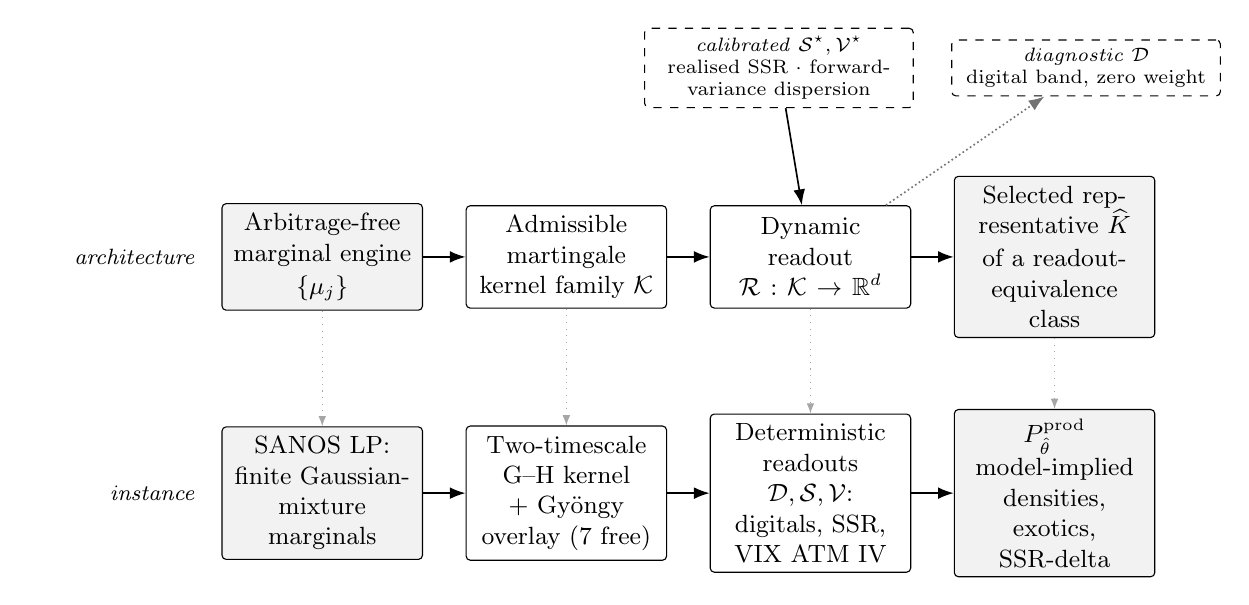
\begin{tikzpicture}[
  font=\small,
  box/.style={draw, rounded corners=1.5pt, align=center, inner sep=3.5pt, minimum height=13mm, text width=23mm},
  io/.style={box, fill=black!5},
  arr/.style={-{Latex[length=2mm]}, semithick},
  rowlab/.style={font=\footnotesize\itshape, align=right, anchor=east, text width=20mm},
  panlab/.style={font=\small, anchor=west, align=left},
  tgt/.style={draw, dashed, rounded corners=1.5pt, align=center, inner sep=3pt, text width=42mm, font=\scriptsize},
  tgt2/.style={tgt, text width=32mm},
  sel/.style={draw, rounded corners=1.5pt, align=center, inner sep=3pt, minimum height=23mm, text width=23mm, font=\scriptsize},
  selme/.style={sel, very thick, fill=black!5}
]
\def\xA{0}\def\xB{3.1}\def\xC{6.2}\def\xD{9.3}
\def\ya{0}\def\yb{-3.0}\def\ys{-6.5}
\def\xL{-3.5}

% ================= PANEL (a) =================
\node[rowlab] at (-1.5,\ya) {architecture};
\node[rowlab] at (-1.5,\yb) {instance};
\node[io]  (a1) at (\xA,\ya) {Arbitrage-free marginal engine\\[1pt]$\{\mu_j\}$};
\node[box] (a2) at (\xB,\ya) {Admissible martingale kernel family $\Kfam$};
\node[box] (a3) at (\xC,\ya) {Dynamic readout $\Rcal:\Kfam\to\R^{d}$};
\node[io]  (a4) at (\xD,\ya) {Selected representative $\widehat K$\\[1pt]of a readout-equivalence class};
\draw[arr] (a1)--(a2); \draw[arr] (a2)--(a3); \draw[arr] (a3)--(a4);
\node[tgt2] (tg) at (\xC-0.4,2.4) {\emph{calibrated} $\mathcal S^\star,\mathcal V^\star$\\
  realised SSR $\cdot$ forward-variance dispersion};
\node[tgt2] (dg) at (\xD+0.4,2.4) {\emph{diagnostic} $\mathcal D$\\ digital band, zero weight};
\draw[arr] (tg)--(a3);
\draw[arr, densely dotted, draw=black!55] (a3)--(dg);
\node[io]  (b1) at (\xA,\yb) {SANOS LP: finite Gaussian-mixture marginals};
\node[box] (b2) at (\xB,\yb) {Two-timescale G--H kernel $+$ Gy\"ongy overlay ($7$ free)};
\node[box] (b3) at (\xC,\yb) {Deterministic readouts $\mathcal D,\mathcal S,\mathcal V$: digitals, SSR, VIX ATM IV};
\node[io]  (b4) at (\xD,\yb) {$P^{\mathrm{prod}}_{\hat\theta}$\\[1pt]model-implied densities, exotics, SSR-delta};
\draw[arr] (b1)--(b2); \draw[arr] (b2)--(b3); \draw[arr] (b3)--(b4);
\foreach \i in {1,2,3,4}{\draw[-{Latex[length=1.3mm]}, draw=black!35, dotted] (a\i.south)--(b\i.north);}

\end{tikzpicture}
\caption{The identification pipeline (upper row) and the instance implemented here (lower row).
The general construction needs only a convex-ordered marginal engine, an admissible martingale-kernel
family~$\Kfam$, and a dynamic readout~$\Rcal$; the kernel is the unknown. Two blocks are
\emph{calibrated}---the coupling readout $\mathcal S$ and the amplitude readout $\mathcal
V$---and what they select is a representative of a readout-equivalence class, not a unique kernel.
The digital band $\mathcal D$ runs the other way: it is emitted and reported at zero loss weight
(dotted), a diagnostic of the leverage overlay rather than a target. Everything to the right of the
kernel is model-implied. The lower row instantiates each stage with the SANOS marginal engine, the
two-timescale Gauss--Hermite kernel with a Gy\"ongy leverage overlay, and the deterministic digital,
skew-stickiness and variance-index readouts.}
\label{fig:architecture}
\end{figure}

The construction separates the marginal level from the relative stochastic-volatility structure.
Conditional on the carried volatility state the intrinsic return law is translation-invariant in log
spot---computationally valuable, but unable in general to connect an arbitrary prescribed marginal
pair---so a deterministic state-dependent leverage overlay supplies the local scaling the fixed
surface implies, while the intrinsic kernel keeps the dispersion, persistence and return--state
dependence the readouts identify. At finite resolution the resulting marginal compatibility is
measured by the digital residual rather than assumed.

The implemented kernel is a parsimonious realisation of that architecture: two carried persistence
timescales and a renewed within-step return branch, with martingality imposed structurally by a
log-sum-exp normalisation. Conditional on the volatility state and the branch the log-return is
Gaussian, so the transition law is a finite Gaussian mixture whose weights and moments are explicit
functions of the parameters, and one-step propagation of the intrinsic kernel is an analytic mixture
update. Finite mixtures have a long history as a tractable smile-consistent
family~\cite{brigo2002}; specifying the transition law directly rather than a driving process has an
architectural analogue in Markov-functional interest-rate
models~\cite{huntkennedypelsser2000}, which share a low-dimensional Markov driver, a deterministic
functional calibration map and an efficient implementation. That analogy is structural---what
selects the kernel here is observed dynamic behaviour.

The readout vector implements those two coordinates and carries a third block that is reported
rather than optimised. $\mathcal S$ is the realised skew-stickiness term structure, read at five
tenors from one week to three months. $\mathcal V$ is the forward-variance dispersion block, whose
market observation is the VIX at-the-money implied-volatility term structure on SPX and a corrected
realised strip off index---related observation operators occupying one slot, not the same quantity.
Only these two enter the objective. The third, $\mathcal D$, is a fixed digital band comparing the
propagated and target marginals: a diagnostic of the leverage overlay's finite-resolution
performance, entering the loss at zero weight. Section~\ref{sec:identification} gives each
observation operator, the measure each lives under, and the identification assumption linking the
pooled physical-measure regression to its within-regime risk-neutral analogue.

The static layer used in the empirical implementation is
SANOS~\cite{buehler2026sanos}. It fits weights only, over a fixed grid of Gaussian bumps in
log-moneyness sharing one bandwidth, each priced by Black--Scholes; its linear program enforces
convex order. The fitted marginal is therefore itself a finite Gaussian mixture---a smoothed grid of
point masses, which the bumps become as the bandwidth vanishes.

That representation is why this engine and not another. The marginal layer arrives in the same class
the kernel propagates, so a mixture updated by a Gaussian-mixture kernel is again a mixture, and the
local variance and its Breeden--Litzenberger density are closed forms on that same object. We retain
those marginals and replace the canonical discrete-local-volatility transition associated with them.
The architecture itself asks only for a convex-ordered marginal engine with an explicit tractable
representation---arbitrage-free surface interpolation~\cite{andreasenhuge2011} and its
mixture-preserving variants~\cite{vandenbergmix2026} supply alternatives---but it is the closure
under propagation that keeps every readout a finite sum.


\subsection{How existing methods select the kernel}
\label{sec:landscape}

Other constructions select the same missing law by other means. \emph{Process-first}
models---Heston~\cite{heston1993}, SABR~\cite{hagan2002}, the Bergomi
family~\cite{bergomi2009,bergomi2016}, rough
volatility~\cite{gatheral2018rough,bayerfrizgatheral2016}---specify state dynamics and derive the
kernel, so smile and smile dynamics are encoded together. \emph{Local projection} draws the dynamics
from the marginals: Dupire local volatility~\cite{dupire1994} and the contemporaneous implied
trees~\cite{dermankani1994,rubinstein1994} are the limiting case in which the static surface
determines the dynamic law---so its skew-stickiness is pinned by the static skew, near the
Doeff--Kamal value under an empirical $\tau^{-1/2}$ scaling~\cite{doeffkamal2012}, while the measured
SPX term structure is materially maturity-dependent. \emph{Stochastic-local volatility}~\cite{jex1999,lipton2002,ren2007}
fixes a backbone and identifies a leverage function through Gy\"ongy's
projection~\cite{gyongy1986}, by particle or learning-based schemes~\cite{guyonhl2012,cuchiero2020},
with existence known in the regime-switching case~\cite{jourdain2020};
the leverage recovers the marginal projection, while the remaining conditional dynamics stay
backbone-dependent. \emph{Transport and entropy} methods---Bass
constructions~\cite{conzehl2021,qin2024bass}, martingale optimal
transport~\cite{backhoff2020,guo2022ot}, martingale Schr\"odinger bridges~\cite{guyon2025siam}---impose
marginal or market-price constraints and select an admissible law by a variational or entropic
criterion.

A fourth family models the observable surface \emph{directly}: market models of implied volatility
posit surface dynamics and derive the no-arbitrage drift restrictions those dynamics must
satisfy~\cite{schonbucher1999,contdafonseca2002}, and recent work learns the joint dynamics of
liquid option prices under no-arbitrage constraints~\cite{cohenreisingerwang2021}. Selecting
dynamics from observed surface behaviour is therefore not new; what differs is the object carried.
Those models evolve the surface, so static no-arbitrage is a constraint their dynamics must respect
at every date, whereas the marginals here are fixed once by a convex-ordered engine and the unknown
is the kernel between them.

In each family the smile response follows from the chosen process, projection, or optimality
principle, and the empirical consequence is measurable. Calibrating two-factor Bergomi, rough
Bergomi, rough Heston and Heston as closely as possible to the same SPX smile, \cite{bourgey2024}
finds SSR term structures that all deviate materially from the market's, and concludes that
roughness alone does not change the joint spot--volatility dynamics enough to close the gap;
\cite{frizgatheral2024} supplies the analytic counterpart, a model-free expression for the SSR whose
short-time limit is $H+\tfrac32$ rather than the diffusive $2$. The statistic can also be targeted
directly: the two-factor Quintic OU model~\cite{abijaber2025} calibrates to SPX at-the-money
volatility, skew and SSR term structures, and separately to the joint SPX--VIX smiles under a
penalty holding the model SSR inside $[0.9,2.0]$. One qualification shapes what is claimed below:
such comparisons are drawn against point estimates of a windowed realised SSR carrying no sampling
band, whereas every fit here is reported against its own displayed precision scale, which is the
target's joint-HAC standard error at every date but one (Appendix~\ref{app:hac}).

\paragraph{Adjacent joint SPX--VIX calibration.} Joint SPX--VIX calibration addresses a related but
different inverse problem. Guyon imposes SPX-smile, VIX-future and VIX-smile constraints and selects
a minimum-relative-entropy law~\cite{guyon2024fs,guyon2025siam}; Guo, Loeper, Obl\'oj and Wang
formulate finite SPX and VIX price constraints through semimartingale optimal
transport~\cite{guo2022siam}; and Che et al.\ derive first-order risk perturbations around an
entropically calibrated SPX--VIX coupling, using the SSR to transmit SPX shocks to the VIX
side~\cite{che2026pot}. SANOS-Evolve does not seek to reproduce a variance-index market. It fixes
each underlying's marginal chain and calibrates a restricted explicit kernel to skew-stickiness and
a softly weighted forward-variance-dispersion readout. VIX at-the-money implied volatility supplies
that observation for SPX; off index, a corrected realised proxy built from the underlying's own
option strip fills the same slot, and variance-index futures are not separate calibration
constraints. The distinction that matters is therefore joint cross-market calibration versus
portable readout-based kernel calibration, not competing solutions to one fitting problem.

\subsection{Contributions and findings}

The paper makes three contributions.

\begin{enumerate}
  \item \textbf{Dynamic-readout identification of a stochastic lift.}
    We develop a selection principle for smile dynamics: conditional on an
    independently fitted marginal surface, the latent transition kernel is
    calibrated directly to the two complementary leading-order readouts
    motivated above, and what it selects is a readout-equivalence class. A
    deterministic leverage overlay supplies the local variance level, while
    the kernel controls the relative stochastic-volatility states, their
    persistence, and their dependence on the return innovation.

  \item \textbf{An explicit finite realization and approximation
    foundation.}
    We construct a two-timescale Gaussian-mixture martingale kernel with
    structural fibrewise normalization, analytic one-step mixture
    propagation, and deterministic finite-sum SSR and variance-index
    readouts. Two propositions accompany the construction---leverage and finite-kernel
    stability (Proposition~\ref{prop:stability}) and dynamic-readout regularity
    (Proposition~\ref{prop:readout})---proved in Appendix~\ref{app:density}.

  \item \textbf{Cross-regime evidence and identified limits.}
    Across nine SPX regimes from 2012 to 2024, one uniform protocol places
    the realised SSR term structure within every year's HAC sampling band
    ($0.9$--$3.1\%$ RMS) and fits the VIX ATM implied-volatility term structure to
    $1.8$--$9.2\%$ RMS. An NDX study using own-strip and realised
    forward-variance observations preserves the SSR fit but exposes a
    steep-decay limitation in the variance-of-variance term
    structure. A smile-roll replay---a residual-variance proxy, not
    traded profit and loss---suggests that the benefit of a smile-aware
    adjustment is stability relative to a trailing realised regression
    rather than superior short-horizon forecasting; a fixed ratio
    performs similarly.
\end{enumerate}

The baseline is an ATM-dynamics model: it targets the level response
summarized by SSR and one forward-variance distributional readout, with VIX
entering as a softly weighted observation rather than as a joint calibration
target. Its diffusive finite-factor structure does not reproduce rough
$T\downarrow0$ scaling, and translation invariance excludes spot-level
dependence of conditional smile shape beyond the latent-regime channel.
Section~\ref{sec:discussion} evaluates those limits against the evidence.

%=============================================================================
\section{Identification architecture and guarantees}
\label{sec:architecture}


The marginal engine supplies an arbitrage-free spot law at every listed maturity. The dynamic
unknown is a transition kernel on a lifted spot--volatility state, whose role is not to refit the
vanilla surface but to select a conditional coupling whose observable dynamics agree with the chosen
readouts. This section defines those objects and separates the ideal admissible problem from the
finite-resolution construction used in calibration.

\subsection{The identification problem}

Fix a pricing date and maturities $T_0<T_1<\dots<T_M$ with forwards $F_j$ and discount
factors $D_j$, and work in log-moneyness $z=\log(S/F)$. Four objects.

\emph{A fixed marginal chain.} An external convex procedure returns arbitrage-free spot
laws $\{\mu^Z_j\}_{j=0}^{M}$, increasing in convex order, with an explicit finite mixture
representation. They are fixed once and are not re-fitted when the dynamic targets change.

\emph{A lifted source law.} The kernel acts on a lifted state $X_j=(Z_j,U_j)$ carrying a
latent volatility regime, with law $\widehat\mu_j(\dd z,\dd u)$ whose spot projection is
the engine's output, $\pr^Z_{\#}\widehat\mu_j=\mu^Z_j$. What is transported from one
maturity to the next is $\widehat\mu_j$; the engine pins only its projection. A spot
marginal cannot be pushed through a kernel whose source carries a latent volatility state.

\emph{The ideal family, and the implemented object.} The \emph{ideal} family $\Kfam$ is the set of Markov kernels
$\cK_j(x,\dd y)$ on the lifted state that are positive, normalised, martingale in the
forward-normalised spot on every fibre, and---together with a deterministic leverage
overlay---propagate $\mu^Z_j$ to $\mu^Z_{j+1}$. The implementation does not sit in it, so the
implemented object is not a kernel at all. It is a \emph{law-evolution pipeline}
$P^{\mathrm{prod}}_\theta$: an overlaid finite kernel applied to a mixture, followed by the
recompression projection of Section~\ref{sec:recompress}, which maps laws to laws and is not a
Markov kernel. The pipeline is indexed by $\theta\in\Theta_{\mathrm{prod}}$, the box of
Section~\ref{sec:empirical}. Section~\ref{sec:admiss} says what $P^{\mathrm{prod}}_\theta$ retains
of admissibility and what it does not.

\emph{A dynamic readout.} A map $\Rcal$ returning the finite vector of quantities the calibration
actually measures, defined on a kernel or on a pipeline alike. Identification is the inverse
problem
\begin{equation}\label{eq:idprob}
  \widehat{K}\;\in\;\arg\min_{K\in\Kfam}
  \bigl\|W\bigl(\Rcal(K)-\Rcal^{\star}\bigr)\bigr\|_2^{2},
\end{equation}
in the ideal statement, over kernels, and
\begin{equation}\label{eq:idprob-prod}
  \widehat\theta\;\in\;\arg\min_{\theta\in\Theta_{\mathrm{prod}}}
  \bigl\|W\bigl(\Rcal_{\mathrm{cal}}(P^{\mathrm{prod}}_\theta)
      -\Rcal_{\mathrm{cal}}^{\star}\bigr)\bigr\|_2^{2}
\end{equation}
as implemented---over \emph{parameters} indexing the pipeline, and over the calibrated blocks only,
since $\mathcal D$ carries zero weight. Every fitted object in this paper
solves~\eqref{eq:idprob-prod}; \eqref{eq:idprob} is the problem it approximates. Here $\Rcal^{\star}$ is the observed targets and
$W$ a fixed weighting;
Section~\ref{sec:identification} writes $\Rcal$ out in full. Figure~\ref{fig:architecture}
sets this architecture beside the instance implemented here and against the standing
answers to the selection question.

\subsection{Ideal and finite-resolution admissibility}
\label{sec:admiss}
\begin{definition}[Admissible kernel]
Fix the lifted source law $\widehat\mu_j(\dd z,\dd u)$ of Section~\ref{sec:architecture} and the target spot marginal
$\mu^Z_{j+1}$. A Markov kernel $\cK_j$ on the lifted state is \emph{admissible} if
\begin{equation}
\cA_j\bigl(\widehat\mu_j,\mu^Z_{j+1}\bigr)=\Big\{\cK_j:\ \cK_j\ge 0,\ \cK_j\mathbf 1=1,\
\E[e^{Z_{j+1}}\mid X_j=x]=e^{Z_j}\ \forall x,\
\pr^Z_{\#}\bigl(\widehat\mu_j\cK_j\bigr)=\mu^Z_{j+1}\Big\}.
\label{eq:admissible}
\end{equation}
The conditions are, in order: positivity, normalisation, the (forward-normalised)
martingale property, and exact propagation of the \emph{spot} marginal.
\end{definition}

\begin{definition}[Finite-feature marginal compatibility]
\label{def:eps-admissible}
The production chain is not an element of $\cA_j$, and we do not claim membership of a Wasserstein
ball around it. Two of the four conditions in~\eqref{eq:admissible} hold outright---positivity and
normalisation---and the martingale condition holds in the weakened form
\begin{equation}
  \E\bigl[e^{Z_{j+1}}\mid\cG_j\bigr]=e^{Z_j},
\label{eq:eps-admissible}
\end{equation}
with $\cG_j$ the $\sigma$-algebra the implementation conditions on (the component index and the
price abscissa of~\eqref{eq:relock-state}) and \emph{before} the recompression projection of
Section~\ref{sec:recompress}, which preserves mass and the unconditional forward only. The fourth
condition, exact propagation of the spot marginal, is replaced not by a metric bound but by a
\emph{finite-feature discrepancy}: the seven-threshold digital vector of Section~\ref{sec:rung},
together with the call-price and implied-volatility residuals at the quoted strikes. These are what
Section~\ref{sec:empirical} reports.
\end{definition}

\noindent The natural metric would be $W_1$ on the forward-normalised marginals, which in one
dimension is
\begin{equation}
  W_1(\mu,\nu)=\int_0^{\infty}\bigl|F_\mu(K)-F_\nu(K)\bigr|\,\dd K
  =\int_0^{\infty}\bigl|\partial_K C_\mu(K)-\partial_K C_\nu(K)\bigr|\,\dd K,
  \label{eq:w1-digital}
\end{equation}
the second equality because $\partial_K C_\mu(K)=F_\mu(K)-1$ for undiscounted calls---so $W_1$ is
the total variation across strikes of the call-price difference. A finite set of quoted strikes does
not resolve that total variation, so we report the discrepancy we can measure and make no claim
about $W_1$.

\begin{theorem}[No static arbitrage]
\label{thm:noarb}
Let $\{\mu_j\}_{j=0}^M$ be probability measures on $(0,\infty)$ with
$\E_{\mu_j}[S]=F_j$. Assume their forward-normalised laws $\tilde\mu_j=\law(S_{T_j}/F_j)$ are
increasing in convex order, $\tilde\mu_0\cxle\tilde\mu_1\cxle\cdots\cxle\tilde\mu_M$.
If $\cK_0,\dots,\cK_{M-1}$ are admissible (each $\cK_j\in\cA_j$), then for any initial
\emph{lifted} law $\widehat\mu_0$ with $\pr^Z_{\#}\widehat\mu_0=\mu^Z_0$, the lifted chain
$\widehat\mu_{j+1}=\widehat\mu_j\cK_j$ satisfies $\pr^Z_{\#}\widehat\mu_j=\mu^Z_j$ for every $j$,
and $e^{Z_j}$ is a martingale in the lifted filtration---so the discounted underlying is a
martingale with one-dimensional marginals exactly $\{\mu_j\}$. The induced call surface
$C_j(K)=D_j\int(s-K)^+\mu_j(\dd s)$ is then free of strike (butterfly) and calendar static
arbitrage. Moreover $\cA_j\neq\emptyset$ for every $j$.
\end{theorem}

\begin{proof}[Proof sketch]
\emph{Strike no-arbitrage.} For each $j$, $\mu_j$ is a probability measure with
$\E_{\mu_j}[S]=F_j$; hence $C_j(K)=D_j\int(s-K)^+\mu_j(\dd s)$ is convex and
non-increasing in $K$ with the correct bounds, which is equivalent to absence of
butterfly arbitrage~\cite{breeden1978}.

\emph{Martingale and marginals.} Admissibility gives $\E[e^{Z_{j+1}}\mid X_j=x]=e^{Z_j}$ for
every lifted state $x$, so $e^{Z_j}$ is a martingale in the lifted filtration. It also gives
$\pr^Z_{\#}(\widehat\mu_j\cK_j)=\mu^Z_{j+1}$; propagation happens on the lifted law,
$\widehat\mu_{j+1}=\widehat\mu_j\cK_j$, and only its projection is pinned. Starting from
$\pr^Z_{\#}\widehat\mu_0=\mu^Z_0$, induction gives $\pr^Z_{\#}\widehat\mu_j=\mu^Z_j$ for all $j$,
so the spot marginals are exactly $\{\mu_j\}$ and the discounted underlying is a martingale.

\emph{Calendar no-arbitrage.} A martingale transition implies, by conditional Jensen,
that the forward-normalised marginals are increasing in convex order,
$\tilde\mu_j\cxle\tilde\mu_{j+1}$, which is equivalent to absence of calendar
arbitrage for the call surface.

\emph{Existence.} By Strassen's theorem~\cite{strassen1965,beiglbock2013} a martingale kernel $q$
on the forward-normalised \emph{spot} coordinate with $\mu^Z_j q=\mu^Z_{j+1}$ exists iff
$\tilde\mu_j\cxle\tilde\mu_{j+1}$, and SANOS enforces that convex order across maturities. Strassen
returns a spot object, so it must be lifted before it is an element of $\cA_j$. Disintegrate the
coupling as $q_z(\dd z')$, let the transition ignore the current latent label, and attach any
probability law $\eta_{z'}(\dd u')$ for the next one:
\begin{equation}
  \cK_j\bigl((z,u),\dd(z',u')\bigr)=q_z(\dd z')\,\eta_{z'}(\dd u').
  \label{eq:strassen-lift}
\end{equation}
This is non-negative and normalised; it is fibrewise a martingale, since
$\int e^{z'}q_z(\dd z')=e^{z}$ for every $u$; and for any $\widehat\mu_j$ projecting to $\mu^Z_j$,
$\pr^Z_{\#}(\widehat\mu_j\cK_j)=\mu^Z_j q=\mu^Z_{j+1}$. Hence $\cA_j\neq\emptyset$.
\end{proof}

\noindent The content is that the
no-arbitrage \emph{claim attaches to the admissible set}, and that the set is nonempty
precisely because SANOS delivers marginals in convex order (Strassen). The discrete-local-volatility transition associated with the SANOS
parameterisation~\cite{buehler2026sanos} becomes an element of $\cA_j$ once embedded in the
lifted state---for instance with latent labels drawn independently of the return---and it is
the rigid element the introduction set out to replace. The two calibrated readouts of
Section~\ref{sec:identification} \emph{select a different, controllable element} of $\cA_j$ in the
ideal statement, and they never replace the set. What is fitted is not that element: the production
pipeline is not in $\cA_j$ at all, since it satisfies
the martingale condition at its own numerical state and before recompression, and replaces exact
marginal propagation by the finite-feature discrepancy of
Definition~\ref{def:eps-admissible}. $\cA_j$ is the ideal object the construction targets, not a set
the implementation is claimed to sit in.

One question remains before any particular kernel is written down: is the class we are about to
restrict to rich enough to be worth restricting? The useful form of that question is not density
among admissible martingale kernels but whether the family's \emph{readout image} covers the
behaviour the market shows---a finite-dimensional question, answered by the attainable-range
experiment of Section~\ref{sec:synth} and the nine-regime panel of Section~\ref{sec:spx}.
Table~\ref{tab:exactness} records which layer every later claim attaches to.

\subsection{Structural guarantees and approximation layers}
\label{sec:exactness}

Each layer of the construction carries a property that holds exactly, by structure, and a
separate element whose accuracy is finite. Table~\ref{tab:exactness} grades them, and every later
use of ``exact'' names the row it belongs to.

\begin{table}[htbp]
\centering
\small
\begin{tabular}{p{0.20\textwidth} p{0.36\textwidth} p{0.34\textwidth}}
\toprule
Layer & Structural property & Finite-resolution element \\
\midrule
Marginal engine & arbitrage-free finite-mixture surface, convex-ordered &
quote and interpolation error \\[2pt]
Kernel & positivity and normalisation, at every state and parameter value & none \\[2pt]
Martingality & exact at the numerical state~\eqref{eq:relock-state}, \emph{pre-projection} &
recompression preserves mass and the unconditional forward only \\[2pt]
One-step update & analytic finite Gaussian-mixture propagation &
the chosen discrete kernel \\[2pt]
Local-variance level & the continuous relation~\eqref{eq:gyongy} matched to leading order &
the remainder $R^{\,c}_\Delta$ of~\eqref{eq:levremainder-prod}, measured \\[2pt]
Carried factor law & the branch rule is a fixed quadrature, exact in its own moments &
Gaussian closure: the marginal law is a finite mixture, propagated by its moments \\[2pt]
Marginal compatibility & nothing structural: the overlay targets it, no limit theorem is claimed &
finite-resolution digital discrepancy \\[2pt]
Readouts & deterministic fixed-resolution evaluation of the implemented finite functional &
central difference, Newton inversion, quadrature and interpolation \\
\bottomrule
\end{tabular}
\caption{Structural guarantees and finite-resolution layers. The middle column holds
exactly by construction; the right column is measured and reported.}
\label{tab:exactness}
\end{table}

What the construction avoids, relative to classical stochastic-local volatility, is the
continuous-time leverage fixed point.

\section{A finite martingale realization}
\label{sec:kernel}
%=============================================================================

We now construct one tractable member of the admissible architecture. The design has four
steps. A finite branch kernel represents the joint return--state transition; a two-timescale
coefficient map supplies persistence and leverage; a structural normalization enforces
martingality; and a deterministic local-variance overlay aligns the conditional variance level
with the fixed marginal surface. The resulting kernel remains explicit enough to propagate as a
finite Gaussian mixture.

\subsection{A finite martingale kernel}

The state is the lifted pair of Section~\ref{sec:architecture}, written concretely as
\begin{equation}
X_j=(Z_j,U_j),\qquad Z_j=\log(S_{T_j}/F_j),\quad
U_j=\bigl(u^{\mathsf F}_j,u^{\mathsf S}_j\bigr)\in\R^{2},
\label{eq:kernel}
\end{equation}
with $Z_j$ log-spot and $U_j$ two \emph{continuous} latent volatility factors, each standardised to
unit stationary variance. The class of kernels we work in is
\begin{equation}\label{eq:broadkernel}
  \cK\bigl((z,u),(\dd z',\dd u')\bigr)
  =\sum_{\ell=1}^{n_{\mathsf L}} w_\ell\,
    \cN\bigl(\dd z';\,z+d_{\ell}(u),\,V_{\ell}(u)\bigr)\,
    Q_\ell\bigl(u,\dd u'\bigr),
\end{equation}
a finite mixture over a within-step branch index $\ell$ of Gaussian return increments, each branch
carrying its own Gaussian transition $Q_\ell$ of the two factors. Three properties
of~\eqref{eq:broadkernel} do the structural work, and the rest of the paper leans on them
repeatedly.

\emph{Translation invariance of the intrinsic return law.} The spot enters only as the additive
centre of the Gaussian, so the conditional return law---and hence the conditional smile in
moneyness---depends on the factor pair alone, not on the spot level. This is what makes the
intrinsic propagation an exact mixture map, before the marginal overlay reintroduces a
$z$-dependence (Section~\ref{sec:recompress}), and the dynamic readouts deterministic finite sums
(Section~\ref{sec:identification}).

\emph{The branch index mediates return--factor dependence.} A common $\ell$ appears in both the
Gaussian mean and the factor transition $Q_\ell$, so the joint law of return and next factor state
is not a product of its marginals. This is precisely the dependence that leverage and skew-stickiness
measure, and it is why an approximation theorem for this class must control the joint conditional
law rather than the two conditional marginals separately (Appendix~\ref{app:density}).

\emph{Gaussian destination factor law.} Each $Q_\ell(u,\cdot)$ is Gaussian, so a law carried as a
Gaussian mixture in $(z,u)$ maps to another one and every readout reduces to a finite
\emph{quadrature} sum---not to a sum over a latent alphabet, of which there is none.

The two carried factors and the within-step branch play different roles, and the distinction
matters throughout:

\begin{table}[htbp]
\centering\small
\begin{tabular}{c c p{0.52\textwidth}}
\toprule
Index & Persisted across steps? & Economic role \\
\midrule
$u^{\mathsf F}$ & yes (continuous) & fast volatility factor; the decaying short end of the
skew-stickiness term structure \\[2pt]
$u^{\mathsf S}$ & yes (continuous) & slow volatility factor; the sustained long-end floor \\[2pt]
$\ell$ & no (renewed each step) & within-step return branch; carries the instantaneous skew and
the return--factor coupling \\
\bottomrule
\end{tabular}
\caption{Roles of the two carried factors and the within-step branch. Sans-serif
$\mathsf F,\mathsf S,\mathsf L$ name them. Only the branch $\ell$ carries a node count,
$n_{\mathsf L}$: the two persistent factors are continuous and are propagated as Gaussian moments
rather than on abscissas (Section~\ref{sec:recompress}), so they have no node count of their own.}
\label{tab:indices}
\end{table}

\paragraph{Spot marginal versus lifted law.} The kernel acts on the joint state, so its one-step
law is a lifted joint $\widehat\mu_j(\dd z,\dd u)$, whereas the marginal engine supplies only the
spot marginal $\mu_j^Z(\dd z)=\int_{\R^2}\widehat\mu_j(\dd z,\dd u)$. The first maturity is lifted
with the stationary bivariate factor law $\pi$ of~\eqref{eq:statcorr}; thereafter the joint is
carried by the propagation. Throughout, $\mu_j\cK_j=\mu_{j+1}$ abbreviates the match of \emph{spot} marginals
after propagation of the lifted law, $\pr^Z_{\#}(\widehat\mu_j\cK_j)=\mu^Z_{j+1}$.

Equation~\eqref{eq:broadkernel} admits unrestricted weights, drifts and variances; the
implementation below restricts them to an eight-coefficient image, seven of them fitted. Two scope points belong here rather
than in the appendix. Appendix~\ref{app:density} establishes stability and readout continuity for
the overlaid finite kernel, and \emph{no} approximation-theoretic claim is made for the family: what
that image reaches is answered by measurement (Sections~\ref{sec:synth}
and~\ref{sec:heldout}), not by a density theorem. And the two operations the production chain
performs at \emph{every} step---evaluating the leverage overlay by collocation at finitely many
price abscissas (Section~\ref{sec:fusion}), and recompressing the propagated mixture back to a fixed
component budget (Section~\ref{sec:recompress})---appear in no result of that appendix, which is
stated throughout at a fixed numerical pattern (Remark~\ref{rem:fixed-pattern}). Their effect is
measured (Section~\ref{sec:empirical}) rather than bounded.

\subsection{The two-timescale specialization}
\label{sec:twoscale}

The volatility state is a baseline plus a \emph{fast} and a \emph{slow} mean-reverting factor, the
two-factor Bergomi picture~\cite{bergomi2009,bergomi2016}. Conditional on that state the one-step
log-return is Gaussian, but its mean and variance are functions of a continuous latent state, so the
kernel is an integral over the factors rather than a finite mixture. The remedy is quadrature---
applied to the factors' \emph{effect} on the log-variance, not to the factors themselves, which stay
continuous throughout. An $n$-point
Gauss--Hermite rule represents $\cN(0,1)$ by nodes $\zeta_l$ and weights $w_l$ reproducing its
moments through order $2n-1$,
\begin{equation}
\E_{\cN(0,1)}[g]=\int g(\zeta)\,\frac{e^{-\zeta^2/2}}{\sqrt{2\pi}}\,\dd\zeta
   \ \approx\ \sum_{l=1}^{n} w_l\,g(\zeta_l)\qquad(\text{exact for }\deg g\le 2n-1),
\label{eq:gh}
\end{equation}
so replacing each continuous latent quantity by its nodes turns the integral into a finite sum,
each node a volatility scenario. The nodes, base log-weights $\eta^{\mathsf F},\eta^{\mathsf S}$
and within-step weights $w_l=\softmax(\eta^{\mathsf L})$ are \emph{fixed} quadrature constants.

Eight structural knobs
$\bth=(\nu_{\mathsf{F}},\nu_{\mathsf{S}},\nu_{\mathsf{L}},\lambda_{\mathrm{skew}},
\rho_{\mathsf{F}},\rho_{\mathsf{S}},\kappa_{\mathsf{F}},\kappa_{\mathsf{S}})$ determine every
coefficient in~\eqref{eq:broadkernel}; the level $\bar\gamma$ is a ninth coefficient but is
\emph{solved} rather than fitted, from the reference-variance condition~\eqref{eq:gbar} below.

Each carried factor is a standardised Gaussian \textup{AR(1)},
\begin{equation}
u^{\mathsf F}_{j+1}=\kappa_{\mathsf F}u^{\mathsf F}_j+\sqrt{1-\kappa_{\mathsf F}^{2}}\;
  \varepsilon^{\mathsf F}_{j+1},
\qquad
u^{\mathsf S}_{j+1}=\kappa_{\mathsf S}u^{\mathsf S}_j+\sqrt{1-\kappa_{\mathsf S}^{2}}\;
  \varepsilon^{\mathsf S}_{j+1},
\label{eq:ar1}
\end{equation}
with standard normal innovations, so each has unit stationary variance and $\kappa$ is
\emph{exactly} the one-step autocorrelation, $|\kappa|<1$. This is the \emph{continuous-shock
idealisation}. Production replaces the branch part of each innovation by the finite
Gauss--Hermite rule of~\eqref{eq:gh}: conditional on a branch the factor step is Gaussian, but
marginally the carried law is a finite Gaussian \emph{mixture}, and every ``Gaussian'' statement
below---the bivariate stationary law of~\eqref{eq:statcorr}, the $k$-step law
of~\eqref{eq:kstep}---is that idealisation, realised by matching moments and closing the recursion
in the Gaussian family. The closure is a quadrature approximation, not an identity, and its error is
\emph{not} measured here: the refinement study of Section~\ref{sec:realdata} varies node counts and
the recompression budget, which is a different comparison. Quantifying the closure would mean
propagating the full mixture against the moment-closed recursion, and we do not report it. The leverage is a correlation between
those innovations and the branch variable $\zeta^{\mathsf L}_\ell$ that drives the return,
\begin{equation}
\operatorname{corr}\bigl(\varepsilon^{\mathsf F}_{j+1},\zeta^{\mathsf L}_\ell\bigr)=\rho_{\mathsf F},
\qquad
\operatorname{corr}\bigl(\varepsilon^{\mathsf S}_{j+1},\zeta^{\mathsf L}_\ell\bigr)=\rho_{\mathsf S},
\label{eq:lev}
\end{equation}
leaving each factor an idiosyncratic innovation variance $(1-\kappa^2)(1-\rho^2)$. This is the
return--factor channel of~\eqref{eq:broadkernel}: a branch carrying a large negative return also
tilts both factors, and it does so through the \emph{innovation} rather than through log-spot.

The two factors enter the return law only through the scalar combination
$x_j=\nu_{\mathsf F}u^{\mathsf F}_j+\nu_{\mathsf S}u^{\mathsf S}_j$, so the branch variance and the
within-step skew tilt are
\begin{align}
V_{\ell}(u)&=\exp\!\big(\bar\gamma+x_j+\nu_{\mathsf{L}}\,\zeta^{\mathsf{L}}_\ell\big)\Delta_j,
  &&\text{(two-factor variance)},\label{eq:Vell}\\
\widetilde m_{\ell}(u)&=-\tfrac12 V_{\ell}(u)
  +\lambda_{\mathrm{skew}}\,\zeta^{\mathsf{L}}_\ell\,\sqrt{V_{\ell}(u)},
  &&\text{(instantaneous mean-tilt / skew)},
\end{align}
the drift $d_\ell$ of~\eqref{eq:broadkernel} following from $\widetilde m_\ell$ by the martingale
lock~\eqref{eq:mg-norm}. Only $x_j$ is integrated by quadrature, at $n_{\mathsf X}$ nodes; the
factors themselves are never placed on abscissas. One derived quantity recurs throughout: the
\emph{full} one-step increment variance at a factor state,
\begin{equation}
  \overline V(u)=\E_\ell\bigl[V_\ell(u)\bigr]+\Var_\ell\bigl(\widetilde m_\ell(u)\bigr),
\label{eq:Vbar}
\end{equation}
the law of total variance applied across branches---the within-branch term plus the mean spread the
skew tilt creates. It is what the level condition, the leverage overlay and the forward-variance
readout all measure.

Under~\eqref{eq:ar1}--\eqref{eq:lev} the stationary factor law is bivariate normal with unit
marginals and correlation
\begin{equation}
c=\frac{\sqrt{(1-\kappa_{\mathsf F}^{2})(1-\kappa_{\mathsf S}^{2})}\;
        \rho_{\mathsf F}\rho_{\mathsf S}}{1-\kappa_{\mathsf F}\kappa_{\mathsf S}},
\label{eq:statcorr}
\end{equation}
writing $s_\bullet=\sqrt{1-\kappa_\bullet^{2}}$ for the innovation scales. The only channel
coupling the two factors is their shared leverage on the return branch: if either $\rho$ vanishes
they are stationarily independent. The level is then fixed by requiring the
stationary expected one-step variance to match the reference,
\begin{equation}
\E_\pi\bigl[\overline V\bigr]=\sigma_{\mathrm{ref}}^{2}\,\Delta_j ,
\label{eq:gbar}
\end{equation}
which determines $\bar\gamma$ and removes it from the fitted vector.

The parameters separate by role: $\nu_{\mathsf F},\nu_{\mathsf S}$ set the \emph{spread} of the
log-variance across the two factors and $\nu_{\mathsf L}$ its within-step dispersion;
$\lambda_{\mathrm{skew}}$ the \emph{return skew}; $\kappa_{\mathsf F},\kappa_{\mathsf S}$ the
\emph{persistence}; and $\rho_{\mathsf F},\rho_{\mathsf S}$ the \emph{return--factor dependence},
the innovation leverages. A down move tilts the factors toward higher volatility through
$\rho_{\mathsf F},\rho_{\mathsf S}$. Because the leverage enters the innovation around a
\emph{fixed} stationary target rather than shifting that target, the equilibrium volatility is not
a deterministic function of spot: this is genuine stochastic volatility, and the kernel stays
translation-invariant in $z$.

Since $\kappa$ is an autocorrelation it carries an effective rate directly, through the one-step
half-life $-\log 2/\log\kappa$, and needs no separate interpretation. Across the nine SPX fits of
Section~\ref{sec:spx} the ordering $\kappa_{\mathsf S}>\kappa_{\mathsf F}$ holds at every date, with
median half-lives of $0.7$ weeks fast and $52$ weeks slow, so the two timescales the construction
posits are the two the calibration finds.

The finite approximation is not a discretisation of the two persistent factors. They are carried
continuously---each step propagates their means and covariance, and the state passed between steps is
$(\text{weight},\ \mu,\ \sigma,\ m_{\mathsf F},\ m_{\mathsf S},\ V_{\mathsf{FF}},\
V_{\mathsf{SS}},\ V_{\mathsf{FS}})$ per component---so what is finite is the quadrature that
integrates their \emph{combined} effect on the log-variance, the within-step branch count
$n_{\mathsf L}$, the price sub-abscissas, and the recompression budget. Production values and the
measured readout sensitivity are reported with the empirical protocol in
Section~\ref{sec:empirical}.

\subsection{Structural martingality and the marginal overlay}
\label{sec:fusion}\label{sec:decouple}

Martingality is enforced twice: once on the intrinsic kernel, and again after the market-level
overlay that rescales its variance. The first is stated for the \emph{ideal} construction, at a
fixed latent state; the second is what the implementation performs, and it conditions on the
numerical state instead. The difference is spelled out below and is not cosmetic.

\paragraph{Stage 1: the intrinsic kernel (ideal).} The within-step drift is locked to the forward on
\emph{every} fibre---the kernel's conditional law at a fixed state $(z,u)$, with
$u=(u^{\mathsf F},u^{\mathsf S})\in\R^2$ the continuous factor pair. Writing
$t_\ell(u)=\lambda_{\mathrm{skew}}\zeta^{\mathsf L}_\ell\sqrt{V_\ell(u)}$ for the skew tilt
of~\eqref{eq:Vell}, so that the raw mean is $\widetilde m_\ell(u)=-\tfrac12V_\ell(u)+t_\ell(u)$,
subtract the per-fibre constant
\begin{equation}
A(u)=\log\sum_\ell w_\ell\,\exp\!\big(\widetilde m_\ell(u)+\tfrac12 V_\ell(u)\big)
       =\log\sum_\ell w_\ell\,e^{\,t_\ell(u)},\qquad
d_\ell(u)=\widetilde m_\ell(u)-A(u),
\label{eq:mg-norm}
\end{equation}
so that $\E[e^{Z_{j+1}}\mid z,u]=e^{z}$ exactly at a realised $u$
(Proposition~\ref{prop:mg-ideal}). The shift is a single per-fibre constant,
independent of $z$, stable and differentiable, and it preserves the relative branch tilts that
carry the leverage and the skew-stickiness.

\paragraph{Stage 2: the market-level overlay.} A translation-invariant kernel cannot, on its own,
carry a prescribed marginal chain: its unleveraged propagation has convolution form
$\mu_j\cK_j=\mu_j\ast\eta_j$, which connects only marginal pairs admitting a common increment-law
representation. Matching is restored by one deterministic ingredient, a leverage overlay
$\sigma_{\mathrm{LV}}(z,T_j)$ that rescales the conditional variance. Writing the increment as a
local scale times a unit stochastic-volatility factor,
\begin{equation}
\Var\!\big(\Delta z\mid z,u\big)
=\underbrace{\sigma_{\mathrm{LV}}^2(z,T_j)\,\Delta_j}_{\text{level (market)}}\ \cdot\
\underbrace{\nu_u}_{\text{shape (kernel)},\ \E_\pi[\nu]=1}
\ +\ R^{u}_\Delta,
\qquad
\nu_u=\frac{\bar V_u}{\E_\pi[\bar V]},
\label{eq:decouple}
\end{equation}
with $\bar V_u=\overline V(u)$ of~\eqref{eq:Vbar}: the first two factors are the \emph{target}
decomposition, exact in the continuous-time limit, and $R^{u}_\Delta$ is what the weekly step leaves
\emph{at a fixed latent state}. The implementation does not condition there, so a second remainder
$R^{c}_\Delta$---same algebra, coarser conditioning---appears at~\eqref{eq:levremainder-prod} below
and is the one measured; the two are not the same number, and only $R^{c}_\Delta$ is reported.
Taking $\E_\ell[V_\ell]$ alone mis-scales the leverage by $\sim3\times$ at the calibrated
$\lambda_{\mathrm{skew}}$. The overlay itself is the finite-kernel analogue of the
stochastic-local-volatility leverage relation,
\begin{equation}
\sigma_{\mathrm{LV}}^2(z,T_j)=\frac{\sigma_{\mathrm{Dupire}}^2(z,T_j)}{\E[\nu\mid z]},
\label{eq:gyongy}
\end{equation}
with $\sigma_{\mathrm{Dupire}}$ read from the fixed marginals: a closed-form Gaussian-mixture
call, a Breeden--Litzenberger density, and a calendar finite difference. That difference is well
posed only on a convex-ordered surface, which is what the constraint in Algorithm~\ref{alg:sanos}
is for; the overlay inherits that hypothesis from the marginal engine
(Assumption~\ref{ass:localvar}). Rescaling the variance changes $\E[e^{\Delta z}]$, so the drift
must be re-locked \emph{after} the overlay rather than carried over. Writing
$L(z)=\sigma_{\mathrm{LV}}(z,T_j)/\sigma_{\mathrm{ref}}$, the overlay scales
\begin{equation}
V^{\mathrm{LV}}_{\ell}(u,z)=L(z)^2V_\ell(u),
\qquad
\widetilde m^{\mathrm{LV}}_{\ell}(u,z)=-\tfrac12V^{\mathrm{LV}}_{\ell}(u,z)+L(z)\,t_\ell(u),
\label{eq:relock-lv}
\end{equation}
the variances by $L^2$ and the skew tilt by $L$, and then re-locks. Two things follow, and only the
first is exact.

\emph{The forward is restored exactly, at the state the implementation carries.} The production lock
is taken over the branches \emph{and} the component's own factor quadrature together,
\begin{equation}\label{eq:relock-state}
  A^{\mathrm{LV}}_c(z)=\log\sum_{k}\sum_{\ell}\varpi_k\,w_\ell\,
    \exp\Bigl(\widetilde m^{\mathrm{LV}}_{\ell}(x_{ck},z)+\tfrac12V^{\mathrm{LV}}_{\ell}(x_{ck},z)\Bigr),
\end{equation}
with $x_{ck}$ the component's factor nodes and $\varpi_k$ their weights
(Section~\ref{sec:recompress}), so that $\E[e^{Z_{j+1}}\mid c,z]=e^{z}$ identically
(Proposition~\ref{prop:mg-impl}). That is martingality at the \emph{numerical information
state}---the component index and the price
abscissa---which is the filtration the propagation actually carries. It is not the same as
martingality conditional on a realised $u$: the two coincide only where the component's factor law
is degenerate.

\emph{The conditional variance is matched to leading order, not exactly.} Because variances scale by
$L^2$ while the tilt scales by $L$, the branch dispersion of the drift does not scale as $L^2$. At
the state the implementation conditions on---the component $c$ and the price abscissa $z$
of~\eqref{eq:relock-state}---
\begin{equation}\label{eq:levremainder-prod}
  \Var_{\cK^{L}}\bigl(\Delta Z\mid c,z\bigr)=L(z)^2\,\overline V_{c}+R^{c}_\Delta,
  \qquad
  R^{c}_\Delta=\frac{L^4-L^2}{4}\Var_{k\ell}\bigl(V_\ell\bigr)
    -\bigl(L^3-L^2\bigr)\Cov_{k\ell}\bigl(V_\ell,t_\ell\bigr),
\end{equation}
both terms vanishing at $L=1$, with the moments taken over the \emph{joint} factor-node/branch law
$\varpi_kw_\ell$ that the lock normalises over. The same algebra at a fixed $(z,u)$ gives the same
expression with branch-only moments, but that is a finer information set than the implementation
uses and understates the discrepancy by roughly a factor of two: $R^{u}_\Delta$ and $R^{c}_\Delta$
are different quantities and only the latter is reported. Since $V_\ell=O(\Delta)$ and
$t_\ell=O(\Delta^{1/2})$ the
covariance term dominates and both remainders are $O(\Delta^{3/2})$, so the \emph{relative} error is $O(\Delta^{1/2})$---at
a weekly step that is not automatically negligible, and Section~\ref{sec:realdata} measures it rather
than bounding it. Equation~\eqref{eq:gyongy} is therefore the continuous-time relation the weekly
construction targets, and the finite step realises it to leading order. The re-lock
of~\eqref{eq:relock-state} shifts every branch by one constant, so it restores the forward without
touching $R^{c}_\Delta$. The complete per-step pipeline is
\begin{equation*}
\boxed{\ \text{intrinsic branch law}\ \longrightarrow\ \text{var.\ scaling}\
\longrightarrow\ \text{martingale re-lock}\ \longrightarrow\ \text{overlaid kernel}\ }
\end{equation*}

\paragraph{The division of labour.} This is the decoupling that organises the paper, and it is
stated here once, with the moment it applies to named. \emph{The marginal engine determines the
local variance level; the intrinsic kernel determines the relative regime dispersion and the
return--regime dependence.} The overlay is a variance rescaling, so what it carries is the second
moment: the per-step enforcement is~\eqref{eq:gyongy} followed by the martingale
re-lock~\eqref{eq:relock-state}, which fixes a variance and a mean and constrains nothing beyond them.
The propagated \emph{skew} is therefore not carried by the overlay but generated by the kernel,
through $\lambda_{\mathrm{skew}}$ and the innovation leverages, and Section~\ref{sec:spx} measures
how far short of the target marginal's skew it falls. The
$\pi$-average of~\eqref{eq:decouple} equals $\sigma^2_{\mathrm{LV}}\Delta_j$ up to the finite-step
remainder of~\eqref{eq:levremainder-prod}, so the level is the leverage's responsibility and the kernel
enters only through the unit-mean ratio $\nu_u$.
Positivity and normalisation are structural in the coefficient map and martingality holds at the
numerical state before recompression; marginal compatibility is the overlay's; and calibration therefore fits only dynamic
parameters. The kernel's own level $\bar\gamma$ nearly divides out of $\nu$ and is reset by
$\sigma_{\mathrm{LV}}$, leaving it close to inert; what survives is the \emph{relative} structure of
the factor state---the $\nu_{\mathsf F},\nu_{\mathsf S}$ spread and, through~\eqref{eq:ar1}
and~\eqref{eq:lev}, the autocorrelations and the innovation leverages---which is exactly what the
two calibrated readouts interrogate jointly: the leverages and the spread set the coupling that
$\mathcal S$ measures, the spread and the autocorrelations set the amplitude and persistence that
$\mathcal V$ measures.

The overlay is a composition of three maps---conditional variance, leverage ratio, overlaid
kernel---and each must be stable for approximation of a target-compatible limit to transfer to the
finite-mixture implementation.

\begin{proposition}[Leverage and finite-kernel stability]
\label{prop:stability}
Let the spot-conditional variances converge in $L^2$, $m_n\to m$---which
Assumption~\ref{ass:localvar}(iv) supplies from convergence of the source laws, and which we assume
rather than derive, since conditional expectations are not Lipschitz in adapted
topologies~\cite{beiglbockjmp2022} without further structure. Let the regularised local-variance
input converge, $a_n\to a$, and the coefficient vectors converge, $\theta_n\to\theta$. Then, on the
compact nondegenerate region of Appendix~\ref{app:density}, the leverage ratio $\ell_n^2=a_n/m_n$,
and the overlaid finite kernel $\cK_{\theta_n,\ell_n}$ all converge, the last in integrated
conditional Wasserstein distance. The hypothesis on $\theta_n$ is not decorative: the bound of
Proposition~\ref{thm:kernel} is $C_\theta\|\theta-\tilde\theta\|+C_\ell\|\ell-\tilde\ell\|_{L^2(\mu)}$,
so a coefficient sequence that does not settle gives a kernel sequence that does not either,
however well behaved the source laws and the local variance are.
\end{proposition}

\noindent \emph{Proof idea.} Stability of the conditional mean is not derived here---it is
Assumption~\ref{ass:localvar}(iv), for the reason given there. Granting it, the ratio is stable
because $\nu$ is bounded away from zero on the nondegenerate region; and the overlaid kernel depends on $(\theta,\ell)$ through locally Lipschitz
coefficient maps, a locally Lipschitz log-sum-exp re-lock, and a Gaussian-mixture $W_1$ bound. The
proof is Proposition~\ref{thm:kernel}, at the fixed numerical pattern stated there.

Here $\E[\nu\mid z]$ is the \emph{spot-conditional} average of the unit factor, distinct from the
stationary $\E_\pi[\nu]=1$ and tilted only by the spot--volatility correlation. For marginal
matching---each step re-seeded from the target law---it is close to $1$ and the residual is
discretisation rather than bias. Under multi-step concatenation from a fixed spot (forward
densities, hedging) it is not: the negative leverage tilt correlates high-$\nu$ regimes with low
$z$, so $\E[\nu\mid z{=}0]\approx0.7$ on SPX, and ignoring it under-reads the accumulated ATM level
by ${\sim}10\%$ in volatility over a multi-month chain. The full spot-conditional correction
of~\eqref{eq:gyongy} is therefore retained for absolute-level outputs.

\subsection{Propagation and component control}
\label{sec:recompress}\label{sec:interp}

\paragraph{One-step propagation of the intrinsic kernel is exact.} Translation invariance means the discretised kernel
adds, conditional on a regime, a \emph{fixed} Gaussian increment---constant in the integration
variable---and fixed Gaussians convolve in closed form:
\begin{equation}
\cN(\,\cdot\,;m,v)\ \ast\ \cN(\,\cdot\,;d_{\ell}(x),V_{\ell}(x))
\ =\ \cN\!\big(\,\cdot\,;\,m+d_{\ell}(x),\ v+V_{\ell}(x)\big).
\label{eq:gauss-conv}
\end{equation}
A law carried per component as a Gaussian in $(z,u)$ therefore propagates to a finite mixture of
such Gaussians,
\begin{equation}
\rho_{j+1}(\dd z',\dd u')=\sum_{c}\omega_c\sum_{k,\ell}\varpi_k\,w_\ell\;
\cN\!\big(\dd z';\,m_c+d_{\ell}(x_{ck}),\,v_c+V_{\ell}(x_{ck})\big)\otimes
\cN\!\big(\dd u';\,\mathrm A\,\bar u_{c}+\mathrm b_\ell,\,\Sigma_\ell\big),
\label{eq:gm-closure}
\end{equation}
where $\varpi_k$ are the $n_{\mathsf X}$ Gauss--Hermite weights integrating that component's own
log-variance combination $x=\nu_{\mathsf F}u^{\mathsf F}+\nu_{\mathsf S}u^{\mathsf S}$---itself
Gaussian, since the component is---and $(\mathrm A,\mathrm b_\ell,\Sigma_\ell)$ is the affine
factor update of~\eqref{eq:ar1}--\eqref{eq:lev}, with $\mathrm A=\operatorname{diag}
(\kappa_{\mathsf F},\kappa_{\mathsf S})$ and the branch-dependent mean shift carrying the leverage.
The coefficient variability lives entirely in the outer sum over $(c,k,\ell)$ and never inside a
convolution, so propagation of the \emph{intrinsic} kernel is an exact finite Gaussian-mixture
update, needing no state-space integration, PDE solve or Monte Carlo.

The production chain is not that object, and the difference should not be collapsed. The leverage
overlay of Section~\ref{sec:fusion} scales the branch variances by $L(z)^2$, and that $z$-dependence
is exactly what breaks~\eqref{eq:gauss-conv}: fixed Gaussians convolve, $z$-dependent ones do not.
Each overlaid step is therefore closed by a first-order collocation in $z$ rather than by the
identity above. What survives exactly is structural---positivity and normalisation at every state
and parameter value, and martingality at the numerical state~\eqref{eq:relock-state}---while the
local-variance match carries the remainder~\eqref{eq:levremainder-prod} and marginal propagation is
approximate; Table~\ref{tab:exactness} grades which is which. The collocation residual is moreover a property of
the overlay rather than of the component budget: the Gy\"ongy match is re-imposed at every step, so
this is a first-order approximation error and not a quantity that refining the recompression drives
to zero. (A Monte-Carlo cross-check showed the same collocation biases the multi-step
skew-stickiness when it is applied to the intrinsic branch law instead.)

\paragraph{Why the component count must be controlled.} Equation~\eqref{eq:gm-closure} multiplies
the component count by $n_{\mathsf L}n_{\mathsf X}n_{\mathsf P}$ at each step, where
$n_{\mathsf X}$ is the quadrature over the combined factor state and $n_{\mathsf P}$ the price
sub-abscissas of the leverage evaluation, so composing
$\cK_j\circ\cK_{j+1}\circ\cdots$ over $J$ steps---needed for forward densities, exotics and
intermediate maturities---would leave $(n_{\mathsf L}n_{\mathsf X}n_{\mathsf P})^J$ components. A
single kernel application needs no reduction; concatenation does.

\paragraph{Recompression, and what it does \emph{not} preserve.} Each composed step therefore ends
with a deterministic reduction that holds the budget flat: bands on the two factor means and then on
the price mean, and within each cell a match of mass, mean and variance. It is a \emph{law-level
projection}, not a kernel operation, and the distinction matters. A cell merges descendants
originating in different source states, and the re-lock that follows is a single scalar per chain,
chosen so that the reduced mixture's forward equals the pre-reduction mixture's. What the projection
preserves is therefore mass and the \emph{unconditional} forward; it does not preserve the forward
conditional on each preceding numerical state, and the reduced object is consequently not itself a
martingale kernel. We therefore claim no Strassen or convex-order property along the recompressed
chain: exact martingality is a statement about the pre-projection kernel~\eqref{eq:relock-state}
only, and what the chain carries past the projection is monitored rather than guaranteed. Restoring
the pathwise statement would need conditional recompression---a per-source-cell re-lock---which the
production path does not perform. Multi-step composition therefore stays tractable as an exact
mixture update followed by a deterministic reduced-mixture approximation whose law and martingale
residuals are measured and reported. The per-step pipeline is \emph{propagate} $\to$
\emph{recompress} (budget and global re-lock) $\to$ \emph{leverage} $\to$ re-lock; the recompression
\emph{is} the projection step. The reduction is
never applied across the carried factor bands.

\paragraph{Intermediate maturities.} Because the carried factors are Ornstein--Uhlenbeck, the
\emph{latent} transition operators form a semigroup, $P^U_sP^U_t=P^U_{s+t}$ with mean-reversion
rate $a=-\log\kappa/\Delta$; the overlaid and recompressed production chain does not. Writing
the latent log-variance as $x_t=g_0(t)+X^{\mathsf F}_t+X^{\mathsf S}_t$ separates a
time-inhomogeneous forward-variance level $g_0$ from a time-homogeneous generator, so one
interpolates the one-dimensional curve $g_0$ and constructs intermediate kernels by evaluation,
with no matching optimisation. The carried volatility state is what makes
the construction compose at all; a spot-only kernel, marginalising the volatility state at the
intermediate step, does not, which is why a memoryless kernel needs a matching optimisation.

\subsection{Summary of the construction}

\begin{table}[htbp]
\centering\small
\begin{tabular}{p{0.34\textwidth} p{0.58\textwidth}}
\toprule
Property & Mechanism \\
\midrule
positivity and normalisation & mixture weights and the softmax branch rule \\[2pt]
martingality at the numerical state & log-sum-exp lock~\eqref{eq:relock-state} over branches and factor quadrature \\[2pt]
marginal variance level & conditional leverage overlay~\eqref{eq:gyongy} \\[2pt]
fast/slow memory & the two carried \textup{AR(1)} factors, $\kappa_{\mathsf F},\kappa_{\mathsf S}$ \\[2pt]
spot--volatility comovement & shared branch $\ell$ in the return and in both factor innovations \\[2pt]
tractable propagation & translation-invariant Gaussian increments~\eqref{eq:gauss-conv} \\[2pt]
bounded complexity & deterministic law-level recompression \\
\bottomrule
\end{tabular}
\caption{What each structural feature of the construction delivers.}
\label{tab:construction}
\end{table}

\section{Dynamic readouts and identification}
\label{sec:identification}

Section~\ref{sec:intro} motivates $\mathcal S$ and $\mathcal V$ as complementary coupling and
amplitude readouts of leading-order at-the-money dynamics. This section is the formal counterpart:
it defines their observation operators, names the measure each lives under, states the calibration
map, and gives the equivalence that map induces. One point carries over and is worth stating once
as a design principle rather than a claim---the readout is not a summary of the kernel but the
topology in which it is identified, so a family is rich enough, and an approximation good enough,
only relative to the functionals one intends to read off it.

\subsection{The identification map}

\begin{table}[htbp]
\centering\small
\begin{tabular}{c p{0.22\textwidth} c p{0.24\textwidth} p{0.15\textwidth}}
\toprule
Block & Observation & Measure & Kernel feature primarily constrained & Baseline role \\
\midrule
$\mathcal D$ & marginal digitals & $\Qmeas$ & compatibility of the leverage overlay & diagnostic \\[2pt]
$\mathcal S$ & realised skew-stickiness term structure & $\Prob$ target,
$\Qmeas$ analogue & return--factor leverage and its maturity decay & active \\[2pt]
$\mathcal V$ & VIX ATM implied vol (SPX), realised strip (NDX) & $\Qmeas$ / $\Prob$ &
forward-variance persistence and dispersion & active, softly weighted \\
\bottomrule
\end{tabular}
\caption{What each readout block observes, under which measure, and which part of the kernel it
principally constrains. The attribution is a statement about which coordinates each block is most
sensitive to, not a partition: both calibrated blocks move with most of $\bth$, as
Table~\ref{tab:jac7} shows.}
\label{tab:readouts}
\end{table}

The calibration reads these three blocks and optimises two, so two readout vectors have to be kept
apart,
\[
  \Rcal_{\mathrm{cal}}=(\mathcal S,\mathcal V),\qquad
  \Rcal_{\mathrm{report}}=(\mathcal D,\mathcal S,\mathcal V),
\]
the first what the objective sees, the second what is reported. Exact equivalence is a statement
about the calibrated pair alone,
\begin{equation}\label{eq:readout-equiv}
  K\sim_{\mathrm{cal}}K'\iff\Rcal_{\mathrm{cal}}(K)=\Rcal_{\mathrm{cal}}(K'),
\end{equation}
an idealisation no fit attains. What a fit delivers is membership of a production tolerance class,
stated on the pipeline and with the two blocks kept apart because their tolerances are not the same
kind of quantity:
\begin{equation}\label{eq:tolset}
  \Bigl\{\theta\in\Theta_{\mathrm{prod}}:\
    \bigl\|W_{\mathcal S}\bigl(\mathcal S(P^{\mathrm{prod}}_\theta)-\mathcal S^{\star}\bigr)\bigr\|
      \le\varepsilon_{\mathcal S},\ \
    \bigl\|W_{\mathcal V}\bigl(\mathcal V(P^{\mathrm{prod}}_\theta)-\mathcal V^{\star}\bigr)\bigr\|
      \le\varepsilon_{\mathcal V}\Bigr\}.
\end{equation}
Only $\varepsilon_{\mathcal S}$ carries a sampling-error reading: it is set by the skew-stickiness
target's estimated standard error. The forward-variance target is a single-day $\mathbb Q$ read with
no sampling band, so $\varepsilon_{\mathcal V}$ is a \emph{chosen} calibration tolerance---the
discrepancy we are willing to leave---and nothing about it is statistical. The weightings
$W_{\mathcal S},W_{\mathcal V}$ are the corresponding diagonal blocks of the $W$ introduced below.
Every downstream \emph{identification} claim is a claim about~\eqref{eq:tolset}; densities and exotic prices are computed from one representative of it and
remain representative-specific. Write $\theta\in\Theta\subset\R^{n_\theta}$ for the \emph{free}
parameters, $n_\theta=7$ in production: the eight structural coefficients of
Section~\ref{sec:kernel} less $\rho_{\mathsf S}$, which is pinned, and less the level $\bar\gamma$,
which is not a coefficient of $\theta$ at all but solved from $\sigma_{\mathrm{ref}}$ by the level
match of Section~\ref{sec:fusion}. The three blocks are read on grids that the design fixes but the model does
not: a set $\mathcal{K}_{\mathcal{D}}$ of log-moneyness thresholds and a set
$\mathcal{T}_{\mathcal{S}}=\{T_1,\dots,T_{d_{\mathcal{S}}}\}$ of tenors, both stepped at $\Delta t$,
and a set $\{\tau_1,\dots,\tau_{d_{\mathcal{V}}}\}$ of forward-variance expiries. The readout vector
is then
\begin{equation}\label{eq:objvec}
  \mathcal{R}(\theta)=\bigl(\mathcal{D}(\theta),\,\mathcal{S}(\theta),\,\mathcal{V}(\theta)\bigr)
  \in\R^{d_{\mathcal{D}}}\times\R^{d_{\mathcal{S}}}\times\R^{d_{\mathcal{V}}},
  \qquad d_{\mathcal{D}}=d_{\mathcal{S}}\,|\mathcal{K}_{\mathcal{D}}|,
\end{equation}
of total dimension $d$ as in~\eqref{eq:idprob}, with the blocks
\begin{alignat}{2}
  \mathcal{D}_{jk}(\theta)&=\Pr\nolimits_{\theta}\bigl(X_{T_j}>k\bigr),&\qquad
    &T_j\in\mathcal{T}_{\mathcal{S}},\ k\in\mathcal{K}_{\mathcal{D}},\label{eq:blockD}\\
  \mathcal{S}_j(\theta)&=\SSRmod(T_j;\theta)\ \ \text{from~\eqref{eq:exactssr}},&
    &j=1,\dots,d_{\mathcal{S}},\label{eq:blockS}\\
  \mathcal{V}_i(\theta)&=\ivVIX{}^{\,\mathrm{mod}}(\tau_i;\theta)\ \ \text{from~\eqref{eq:vixatm}},&
    &i=1,\dots,d_{\mathcal{V}}.\label{eq:blockV}
\end{alignat}
Only the last two enter the loss. The instance realises the production
problem~\eqref{eq:idprob-prod} with a diagonal $W$ that vanishes on the $\mathcal D$ block and normalises the surviving residuals by their
own targets, plus one term outside that form---a ridge on $\theta$ rather than on the readout---so the
objective is best given explicitly. With targets $\mathcal{S}^{\star},\mathcal{V}^{\star}$, stage
anchor $\theta^{0}$, per-tenor skew-stickiness weights $\varsigma\in\R^{d_{\mathcal{S}}}$ normalised
to $\overline{\varsigma^2}=1$, ridge weights $\varrho\in\R^{n_\theta}$ and a floor $\varepsilon>0$,
the residual vector is
\begin{equation}\label{eq:resid}
  r(\theta)=\biggl(
    \underbrace{\varsigma_j\,\frac{\mathcal{S}_j(\theta)-\mathcal{S}^{\star}_j}{\mathcal{S}^{\star}_j}}_{j\le d_{\mathcal{S}}},\;
    \underbrace{w\,\frac{\mathcal{V}_i(\theta)-\mathcal{V}^{\star}_i}{\mathcal{V}^{\star}_i}}_{i\le d_{\mathcal{V}}},\;
    \underbrace{\varrho_k\,\frac{\theta_k-\theta^{0}_k}{\max(|\theta^{0}_k|,\,\varepsilon)}}_{k\le n_\theta}
  \biggr),
  \qquad w=w_{\mathrm{vov}}\sqrt{\frac{d_{\mathcal{S}}}{d_{\mathcal{V}}}},
\end{equation}
and the objective is its least-squares cost,
\begin{equation}\label{eq:loss}
\begin{aligned}
  J(\theta)&=\tfrac12\bigl\|r(\theta)\bigr\|_2^{2}\\[2pt]
  &=\underbrace{\tfrac12\sum_{j=1}^{d_{\mathcal{S}}}\varsigma_j^{2}
      \Bigl(\tfrac{\mathcal{S}_j-\mathcal{S}^{\star}_j}{\mathcal{S}^{\star}_j}\Bigr)^{2}}_{\text{skew-stickiness}}
  +\underbrace{\frac{w_{\mathrm{vov}}^{2}d_{\mathcal{S}}}{2d_{\mathcal{V}}}\sum_{i=1}^{d_{\mathcal{V}}}
      \Bigl(\tfrac{\mathcal{V}_i-\mathcal{V}^{\star}_i}{\mathcal{V}^{\star}_i}\Bigr)^{2}}_{\text{forward variance}}
  +\underbrace{\tfrac12\sum_{k=1}^{n_\theta}
      \frac{\varrho_k^{2}(\theta_k-\theta^{0}_k)^{2}}{\max(|\theta^{0}_k|,\varepsilon)^{2}}}_{\text{ridge}},
\end{aligned}
\end{equation}
minimised over the box $\theta^{\mathrm{lo}}\le\theta\le\theta^{\mathrm{hi}}$. The grids, the weights
$w_{\mathrm{vov}},\varsigma,\varrho,\varepsilon$ and the box are design choices of the empirical study and are
given with it in Section~\ref{sec:empirical}; the factor $\tfrac12$ is the least-squares convention,
carried so that the multi-start costs quoted in Appendix~\ref{app:protocol} are on the scale
of~\eqref{eq:loss}.

Four features of~\eqref{eq:loss} are choices rather than conventions. \emph{Residuals are
relative}: a given percentage miss counts the same at every tenor, though the levels differ by an
order of magnitude across $\mathcal{T}_{\mathcal{S}}$. \emph{The forward-variance block is normalised
by its own length}: the factor $\sqrt{d_{\mathcal{S}}/d_{\mathcal{V}}}$ fixes that block's aggregate
weight at $w_{\mathrm{vov}}^{2}d_{\mathcal{S}}$ whatever $d_{\mathcal{V}}$ happens to be, so the
cross-underlying comparison of Section~\ref{sec:ndx} is like-for-like. \emph{The digital block is
absent}, not merely down-weighted (Section~\ref{sec:rung}). \emph{The ridge is not a target}: it
penalises displacement from the stage anchor rather than misfit to data, scaled to each coordinate's
own anchor value, and tames the railing the loosely identified directions would otherwise produce
(Appendix~\ref{app:protocol}).

Two counting conditions follow, and they constrain the design rather than the model. Only the
$\mathcal S$ and $\mathcal V$ blocks carry observations, so the data-bearing residuals number
$d_{\mathcal{S}}+d_{\mathcal{V}}$ and nominal determinacy requires
$d_{\mathcal{S}}+d_{\mathcal{V}}\ge n_\theta$; the ridge adds $n_\theta$ further residuals, but those
are regularisation rather than observation, and can only make
the optimiser well-posed on one. Identifiability asks more than counting. The parameters separate by
role (Section~\ref{sec:kernel}), and so does the evidence: the skew-stickiness term structure is the
primary evidence for the leverages and persistence loadings, the forward-variance term structure for
the regime spreads. Since the kernel carries two timescales, the $\mathcal S$ curve is essentially a
two-rate decay---a short-tenor level, two rates and a relative amplitude---so $\mathcal{T}_{\mathcal{S}}$
must both be large enough to resolve four shape degrees of freedom and \emph{span} both timescales.
A grid confined to tenors short relative to $-1/\log\kappa_{\mathsf S}$ steps leaves the slow factor
constrained only through the ridge, however many points it contains.

\subsection{Marginal compatibility}
\label{sec:rung}

For a propagated mixture $\rho(\dd x)=\sum_i W_i\,\cN(\mu_i,\sigma_i^2)(\dd x)$ the survival
probability at threshold $k$ is the finite sum $\Pr(X>k)=\sum_i W_i\,\Phi((\mu_i-k)/\sigma_i)$,
evaluated on the grid $\mathcal{K}_{\mathcal{D}}$ against the interpolated target marginal at the
corresponding maturity. The resulting $|\mathcal{K}_{\mathcal{D}}|$ survival probabilities per
maturity report what the leverage overlay of Section~\ref{sec:fusion} does and does not achieve at
finite resolution; the grid used here is given in Section~\ref{sec:realdata}.

This block carries \emph{zero weight} in the baseline fits: it belongs in the reported readout
vector but not in the optimised loss, and serves as an acceptance readout. A configuration with a
positive digital weight is used for the decoupling experiment of Section~\ref{sec:empirical}, where
up-weighting $\mathcal D$ degrades the dynamic fit by more than an order of magnitude---which is
itself the evidence that the statics and dynamics are separately
controlled.

\subsection{Skew-stickiness: a within-regime risk-neutral analogue}
\label{sec:ssr}

Three distinct objects are called ``SSR'' in this literature. We name them before computing
anything.

\begin{table}[htbp]
\centering\small
\begin{tabular}{p{0.26\textwidth} p{0.30\textwidth} p{0.34\textwidth}}
\toprule
Object & Where it lives & Role here \\
\midrule
Empirical \emph{pooled} realised-regression $\SSRemp$ &
Calendar-time panel under $\Prob$, no conditioning on the latent state &
The calibration target. \\[2pt]
Instantaneous / leading-order $\SSRinst$ &
Continuous-time asymptotics &
Analytic interpretation, limiting values, and the hedge formula. Never a
fitted quantity. \\[2pt]
Finite-step \emph{within-regime} $\SSRmod$, eq.~\eqref{eq:exactssr} &
The implemented discrete kernel, stationary regime law, under $\Qmeas$ &
The fitted model readout. ``Exact'' scopes the evaluation of this functional, not equality
with the pooled target. \\
\bottomrule
\end{tabular}
\caption{The three skew-stickiness objects. Every occurrence of ``SSR'' in this paper names one
of these three.}
\label{tab:threessr}
\end{table}

\noindent
The empirical target is the pooled regression
$\mathrm{Cov}(\Delta\Sigma_{\mathrm{ATM}}(T),r)/[\mathrm{Var}(r)\,\mathrm{skew}(T)]$, estimated on
the calendar panel with a single intercept; the latent volatility state is neither observed nor
conditioned on. The empirical and model statistics measure the same economic channel but are not identical
functionals: the former is a pooled physical-measure regression, the latter a stationary average of
within-regime risk-neutral covariance and variance. The calibration imposes
\[
  \SSR^{\Qmeas,\,\mathrm{within}}_{\mathrm{mod}}(T)\ \approx\
  \SSR^{\Prob,\,\mathrm{pool}}_{\mathrm{emp}}(T)
\]
as an identifying modelling restriction, not as an equality of functionals.

\paragraph{The two channels.} The sums below run over the $(f,s)$ nodes of the \emph{stationary
quadrature} of the bivariate factor law~\eqref{eq:statcorr}, with $\pi_{fs}$ the corresponding
Gaussian-copula weights. They are quadrature nodes of a continuous law, not states of a finite
alphabet: the construction of Section~\ref{sec:kernel} has none. For each such node $(f,s)$ and
maturity $T$ the routine
precomputes the propagated at-the-money volatility $\sigma(u^{\mathsf F},u^{\mathsf S};z,T)$ on the
fixed factor--spot grid, its slope
$\mathrm{skw}_{f,s}(T)=\partial_z\sigma(u^{\mathsf F}_f,u^{\mathsf S}_s;0,T)$, the leveraged branch means and
variances $(D_{f s\ell},V_{f s\ell})$, the branch weights $w_\ell$, the stationary node weights
$\pi_{f s}$, and the Gauss--Hermite nodes and normalised weights $(z_q,\omega_q)$. With realised
returns $r_{f s\ell q}=D_{f s\ell}+\sqrt{V_{f s\ell}}\,z_q$ and
$\bar r_{f s}=\sum_\ell w_\ell D_{f s\ell}$, the factors take their own \textup{AR(1)} step,
\begin{equation}\label{eq:ustep}
  u^{\mathsf F}_{f\ell e}=\kappa_{\mathsf F}u^{\mathsf F}_f
    +s_{\mathsf F}\bigl(\rho_{\mathsf F}\zeta_\ell
      +\sqrt{1-\rho_{\mathsf F}^{2}}\,\varepsilon^{\perp}_{e}\bigr),
  \qquad
  u^{\mathsf S}_{s\ell e'}=\kappa_{\mathsf S}u^{\mathsf S}_s
    +s_{\mathsf S}\bigl(\rho_{\mathsf S}\zeta_\ell
      +\sqrt{1-\rho_{\mathsf S}^{2}}\,\varepsilon^{\perp}_{e'}\bigr),
\end{equation}
with $(\varepsilon^{\perp},\omega)$ a further Gauss--Hermite rule, applied once per factor because
the innovations are independent \emph{given} the shared branch $\zeta_\ell$. The one-step
at-the-money volatility change is then
\begin{equation}\label{eq:dsigma}
  \Delta\sigma_{f s\ell e e' q}(T)
  =\sigma\bigl(u^{\mathsf F}_{f\ell e},u^{\mathsf S}_{s\ell e'};\,r_{f s\ell q},T\bigr)
   \;-\;\sigma\bigl(u^{\mathsf F}_f,u^{\mathsf S}_s;\,0,T\bigr),
\end{equation}
the first term read off the precomputed surface by trilinear interpolation in the two factor
coordinates and the spot shift. It carries both channels: the \emph{surface} channel, through
evaluation at the realised return, and the \emph{factor} channel, through~\eqref{eq:ustep}, which
moves which slice of the surface is read. No transition matrix between regimes appears: the factor
update is the continuous one of~\eqref{eq:ar1}, and only the surface lookup is discretised. The
readout is the finite sum
\begin{equation}\label{eq:exactssr}
  \SSRmod_T=\frac{\mathcal{C}_T}{Q\,\bar s_T},\qquad
  \mathcal{C}_T=\sum_{f,s}\pi_{f s}\sum_{\ell,e,e',q}w_\ell\,\omega_e\omega_{e'}\omega_q\,
    \Delta\sigma_{f s\ell e e' q}(T)\,(r_{f s\ell q}-\bar r_{f s}),
\end{equation}
normalised by the model's own return variance and average skew,
\begin{equation}
  Q=\sum_{f,s}\pi_{f s}\Bigl[\sum_\ell w_\ell\bigl(D^2_{f s\ell}+V_{f s\ell}\bigr)-\bar r^{\,2}_{f s}\Bigr],
  \qquad
  \bar s_T=\sum_{f,s}\pi_{f s}\,\mathrm{skw}_{f s}(T).
\end{equation}

\paragraph{How far apart are the two functionals?} Both the numerator and denominator
of~\eqref{eq:exactssr} centre \emph{within} each regime, so by the total-covariance and
total-variance identities they differ from the pooled statistic by the between-regime terms
$\Cov(\E[\Delta\Sigma\mid I],\E[r\mid I])$ and $\Var(\E[r\mid I])$. Two independent measurements
bound the gap. Model side: at the calibrated kernels
$\eta^{\Qmeas}_{\mathrm{var}}=0.003$--$0.03\%$ and $\eta^{\Qmeas}_{\mathrm{cov}}=0.05$--$1.2\%$, so
global re-centring would move $\SSRmod$ by at most $1.3\%$. Data side: partitioning the empirical
panel by an observable proxy for the volatility state (the lagged one-month at-the-money
volatility), the between-state share of the covariance reaches $4.7\%$ in terciles and $8.4\%$ in
quintiles, moving the empirical $\SSR$ by a median $0.85\%$ and at most $4.9\%$ over $2012$--$2024$,
at both resolutions inside the sampling band of Appendix~\ref{app:hac}. Neither addresses the
\emph{measure}: the model is a $\Qmeas$-martingale whose only regime-dependent mean return is the
$O(\sigma^2\Delta)$ Jensen correction, whereas the pooled empirical between-state terms can carry
physical drift and variance-risk premium, and it is the leading-order invariance of quadratic
covariation that licenses comparing the \emph{within-state} channels. That protection does not
extend to the higher-moment forward-variance channel, which governs the off-index results of
Section~\ref{sec:empirical}.

\paragraph{What the ratio means for a delta.} The instantaneous object fixes the convention the
$\SSR$ values in this paper are quoted in. For a spot--volatility response coefficient $R$ and skew
$\mathcal{S}$,
\begin{equation}\label{eq:ssr-delta}
  \Delta(R)=\Delta_{\mathrm{BS}}+\mathrm{Vega}\cdot R\,\mathcal{S}/S
\end{equation}
folds the level-induced move of the at-the-money volatility into the Black delta, with $R$ in
$\SSR$ units: $R{=}0$ is the no-roll reference and the variance-minimising choice is $R=\SSR_T$. For
a \emph{fixed-strike} option the smile-roll term shifts this by one unit, giving
$\Delta_{\mathrm{BS}}+\mathrm{Vega}\,(\SSR_T-1)\,\mathcal S/S$, whence sticky-strike is
$\SSR{=}1$~\cite{gatheral2006} and sticky-moneyness $\SSR{=}0$---the reference values against which
Section~\ref{sec:smilemotion} places the calibrated kernel.

\subsection{Forward-variance information}
\label{sec:fwdvar}

As Section~\ref{sec:intro} sets out, the skew-stickiness block constrains coupling but its
normalisation divides out most of volatility's own amplitude. This block reads the forward-variance
distribution directly; on SPX its market observation is the VIX at-the-money implied-volatility term
structure, entering as a softly weighted reading rather than as a jointly calibrated
market---the object of the joint SPX--VIX literature~\cite{guyon2024fs,guo2022siam,che2026pot}.

Because the carried factors are the Gaussian \textup{AR(1)} pair of~\eqref{eq:ar1}, the $k$-step
law of $U$ from any Gaussian state $(m,V)$ today is available in closed form, with no transition
matrix and no matrix power:
\begin{equation}\label{eq:kstep}
\begin{aligned}
  m^{\mathsf F}_k&=\kappa_{\mathsf F}^{k}m^{\mathsf F}_0, &
  V^{\mathsf{FF}}_k&=\kappa_{\mathsf F}^{2k}V^{\mathsf{FF}}_0+\bigl(1-\kappa_{\mathsf F}^{2k}\bigr),\\
  m^{\mathsf S}_k&=\kappa_{\mathsf S}^{k}m^{\mathsf S}_0, &
  V^{\mathsf{SS}}_k&=\kappa_{\mathsf S}^{2k}V^{\mathsf{SS}}_0+\bigl(1-\kappa_{\mathsf S}^{2k}\bigr),
\end{aligned}
\qquad
  V^{\mathsf{FS}}_k=(\kappa_{\mathsf F}\kappa_{\mathsf S})^{k}V^{\mathsf{FS}}_0
   +s_{\mathsf F}s_{\mathsf S}\rho_{\mathsf F}\rho_{\mathsf S}
    \frac{1-(\kappa_{\mathsf F}\kappa_{\mathsf S})^{k}}{1-\kappa_{\mathsf F}\kappa_{\mathsf S}},
\end{equation}
the unit stationary variances of~\eqref{eq:ar1} supplying the constants. The cross term is the
\emph{shared} branch shock accumulating over $k$ steps: $\rho_{\mathsf F}$ and $\rho_{\mathsf S}$
load on the same $\zeta^{\mathsf L}_\ell$, so the two factors do not decouple, and setting
$V^{\mathsf{FS}}$ to zero would make their innovations independent while each stayed correlated with
the return. The thirty-day forward volatility is the window average of the one-step increment variance,
normalised by its stationary value so that $\sigma_{\mathrm{ref}}$ carries the level:
\begin{equation}\label{eq:fwdvar}
  \Upsilon(m,V)^2=\sigma_{\mathrm{ref}}^{2}\,
    \frac{\frac{1}{n_{\mathrm{var}}}\sum_{k=1}^{n_{\mathrm{var}}}\E\bigl[\overline V(U_k)\bigr]}
         {\E_\pi\bigl[\overline V\bigr]},
  \qquad U_k\sim\cN\bigl(m_k,V_k\bigr),
  \qquad n_{\mathrm{var}}=\max\bigl(1,\operatorname{round}(\tfrac{30}{365}/\Delta)\bigr),
\end{equation}
with $\overline V$ the full one-step increment variance~\eqref{eq:Vbar} and $\E_\pi$ that same
functional on the stationary factor law---the normalisation of~\eqref{eq:gbar}, so that $\Upsilon$
returns $\sigma_{\mathrm{ref}}$ on the stationary state by construction. Each
term is evaluated by the combined-factor quadrature of~\eqref{eq:Vell}, since $V_\ell$ depends on
$U$ only through $x=\nu_{\mathsf F}u^{\mathsf F}+\nu_{\mathsf S}u^{\mathsf S}$, itself Gaussian with
mean $\nu_{\mathsf F}m^{\mathsf F}_k+\nu_{\mathsf S}m^{\mathsf S}_k$ and variance
$\nu_{\mathsf F}^2V^{\mathsf{FF}}_k+2\nu_{\mathsf F}\nu_{\mathsf S}V^{\mathsf{FS}}_k
+\nu_{\mathsf S}^2V^{\mathsf{SS}}_k$. Today's state is a state choice rather than a parameter: the
fast factor starts at its mean and the slow level $u^{\mathsf S}_0$ is bisected so that
$\Upsilon\bigl((0,u^{\mathsf S}_0),0\bigr)$ reproduces the observed spot index, under
\texttt{no\_grad} and therefore outside the optimisation. That consumes one observation---the spot
variance index on SPX, the own-strip thirty-day variance-swap rate off it---which is spent on the
state and is not among the residuals counted in Section~\ref{sec:realdata}.
At the option expiry, $n_{\mathrm{opt}}=\max(1,\operatorname{round}(\tau/\Delta))$ steps out, the readout needs the \emph{law} of
$\Upsilon$, and the propagation of Section~\ref{sec:recompress} supplies it: each surviving
component $j$ carries a weight $w_j$, a log-price law $\cN(\mu_j,\sigma_j^2)$, and a conditional
factor law $\cN(m_j,V_j)$ whose moments are~\eqref{eq:kstep} run from that component's own state.
The factor is realised at the expiry, so the index value there is $\Upsilon(u,0)$ at
Gauss--Hermite nodes $u_{j,ab}$ of $\cN(m_j,V_j)$: the residual variance is expanded, not passed
back into~\eqref{eq:fwdvar}, which would turn genuine dispersion of the index into a convexity
correction on its mean. The leverage enters here as well---instantaneous variance is
$\ell(z)^2e^{g}$, so the thirty-day rate carries $\ell$ too---read across the component's own
log-price nodes $z_{j,q}$. Production reads it as a root-mean-square over the variance window
rather than at one slice,
\begin{equation}\label{eq:lamrms}
  \ell_{j,q}\ \propto\ \Bigl(\tfrac{1}{n_{\mathrm{var}}}\sum_{m=0}^{n_{\mathrm{var}}-1}
    \ell_{\,n_{\mathrm{opt}}-1+m}(z_{j,q})^{2}\Bigr)^{1/2},
\end{equation}
normalised to unit weighted mean, because instantaneous variance is $\ell^2e^{g}$ and the index
averages it over $[\tau,\tau+30\text{d}]$: what multiplies is the RMS across those slices, and
consecutive tenors then share $n_{\mathrm{var}}-1$ of them instead of inheriting the ladder's
per-week jumps. With $\omega_{jabq}$ the product of the four weights,
\begin{equation}\label{eq:vixatm}
  X_{jabq}=\ell_{j,q}\,\Upsilon\bigl(u_{j,ab},0\bigr),\quad
  F^{\mathrm{mod}}=\sum\omega_{jabq}X_{jabq},\quad
  C^{\mathrm{mod}}_{\mathrm{ATM}}=\sum\omega_{jabq}\bigl(X_{jabq}-F^{\mathrm{mod}}\bigr)^{+},
\end{equation}
and the at-the-money Black inversion is closed form,
$\ivVIX{}^{\,\mathrm{mod}}
 =(2\sqrt2/\sqrt{\tau})\operatorname{erf}^{-1}
   \bigl(C^{\mathrm{mod}}_{\mathrm{ATM}}/F^{\mathrm{mod}}\bigr)$.
Neither choice is cosmetic. A readout that drops $\ell$ levers the skew-stickiness block but not
this one, so the two blocks would then read different models. And when
$\rho_{\mathsf F}=\rho_{\mathsf S}=0$ the branch shock does not move components at all---every bit
of factor uncertainty sits inside $V_j$---so folding $V_j$ in as convexity would report exactly no
dispersion for a model with unchanged $\nu_{\mathsf F},\nu_{\mathsf S}$.
The market counterpart estimates the variance-index forward from a put--call parity regression over
central strikes and reads the out-of-the-money smile at that forward, so the calibrated
number is an at-the-money implied volatility rather than a generic dispersion parameter.

One qualification belongs with this block: it imposes unconditional forward-variance consistency
only. The conditional identity a genuine joint calibration would require is exactly what reading
rather than jointly fitting forgoes.

\paragraph{Portability.} That weaker formulation is what makes the readout portable. The model
side of the block does not change with the underlying: it is~\eqref{eq:vixatm} in every case, an
at-the-money implied volatility read off the kernel's own forward-variance law. What changes
is the observation that fills the target slot. Where a liquid variance-index option market
exists---among the underlyings here, SPX---that observation is the market counterpart
of~\eqref{eq:vixatm} term for term. NDX has no such market, so the target is the realised volatility
of a constant-maturity variance-swap strip built from the underlying's own options
(Appendix~\ref{app:data}, equation~\eqref{eq:ndxvov}). The two observation operators occupy the same
slot in $\mathcal{R}$ with the same identification role and different measure content, so off index a
residual in that block carries the operator mismatch as well as any kernel error. The consequences
are taken up in Section~\ref{sec:empirical}.

\subsection{Parameter roles and identifiability}

\begin{table}[htbp]
\centering\small
\begin{tabular}{p{0.30\textwidth} p{0.60\textwidth}}
\toprule
Parameters & Principal effect \\
\midrule
$\rho_{\mathsf F},\rho_{\mathsf S}$ & innovation leverage: level of spot--volatility comovement \\[2pt]
$\kappa_{\mathsf F},\kappa_{\mathsf S}$ & factor autocorrelation; the maturity decay of that comovement \\[2pt]
$\nu_{\mathsf F},\nu_{\mathsf S}$ & forward-variance dispersion \\[2pt]
$\lambda_{\mathrm{skew}},\nu_{\mathsf L}$ & within-step return skew and branch spread \\[2pt]
$\bar\gamma$ & variance level; solved from~\eqref{eq:gbar}, not fitted \\
\bottomrule
\end{tabular}
\caption{Which parameters the readouts are principally informative about.}
\label{tab:paramroles}
\end{table}

The kernel is translation-invariant (Section~\ref{sec:kernel}), so the conditional smile depends
only on the regime pair, and skew-stickiness is generated by the \emph{innovation} leverages rather
than by any $z$-coupling: $\rho_{\mathsf F}=\rho_{\mathsf S}=0$ gives no spot--volatility
comovement and $\SSRmod=0$ (sticky-moneyness), while raising them lifts the ratio through the
sticky-strike value and $\kappa_{\mathsf F},\kappa_{\mathsf S}$ shape its term structure---fast for
the decaying short end, slow for the sustained floor. The placement of the leverage is a design
decision with teeth: a Monte-Carlo cross-check showed that coupling the regimes to \emph{spot}
instead makes equilibrium volatility a deterministic function of spot, pinning $\SSRmod\to2$ at long
maturities with no re-tuning, whereas placing it in the innovation breaks that floor while keeping
the readouts deterministic finite sums.

\begin{proposition}[Dynamic-readout regularity]
\label{prop:readout}
On the compact nondegenerate region of Appendix~\ref{app:density}, where liquid strikes are
bounded away from the wings, vega is bounded below at the quoted at-the-money points, and forward variance and average
skew are bounded away from zero, the readout
$\mathcal R=(\mathcal D,\mathcal S,\mathcal V)$ of~\eqref{eq:objvec} is continuous in the kernel, and in the implemented finite parameterisation it
is locally Lipschitz and piecewise $C^1$ in $\bth$.
\end{proposition}

\noindent \emph{Proof idea.} Each block is a finite composition of smooth maps on that region: a
Gaussian-mixture CDF for $\mathcal D$; a matrix polynomial, a square root away from zero, and Black
inversion with vega bounded below for $\mathcal V$; and for $\mathcal S$ a finite sum of bounded
locally Lipschitz factors over two denominators kept away from zero. Kernel-to-readout stability
then propagates along the finite maturity grid. The proof is Theorem~\ref{thm:readout}, via the
propagation recursion of Proposition~\ref{thm:propagation}.

Two consequences matter downstream. The objective is non-convex---implied-volatility inversion, the
stationary law, the leverage, interpolation and the ratio structure of~\eqref{eq:exactssr} all
contribute---so the convexity available for semimartingale optimal
transport~\cite{guo2022ot,backhoff2020} does not transfer. And distinct kernels may produce the same
finite readout vector; that equivalence is measured in Section~\ref{sec:empirical}, and is why the
object carried downstream is the readout rather than the parameter vector.

\section{Validation and empirical evidence}
\label{sec:experiments}\label{sec:empirical}
%=============================================================================

The evidence is organised around four questions. First, does the deterministic implementation
reproduce the finite kernel it is intended to evaluate? Second, does the kernel possess a genuine
dynamic degree of freedom once the marginal surface is held fixed? Third, can the resulting readouts
be fitted across materially different SPX regimes? Fourth, what transfers off SPX, and what does the
resulting smile response imply for a skew-aware delta?

The first two are settled on synthetic ground truth, where the generator is known and every quantity
is computable both in closed form and by simulation (Section~\ref{sec:synth}). The last two are
settled on ORATS end-of-day chains (Sections~\ref{sec:realdata}--\ref{sec:smilemotion}). Target
construction and filters are collected in Appendix~\ref{app:data} and the calibration protocol with
its robustness checks in Appendix~\ref{app:protocol}; the body reports results.

\subsection{Synthetic validation: implementation and attainable range}
\label{sec:synth}

Two things must be checked before any market data is used, and only a known generator can check
them: the first validates the computation, the second validates the economic degree of freedom the
whole construction rests on. Both run at a fixed reference generator $\bth_0$---the eight
coefficients of Section~\ref{sec:twoscale} with $\bar\gamma$ solved and $\rho_{\mathsf S}$ at zero,
calibrated once to canonical SPX term-structure targets---on a synthetic arbitrage-free
chain. The decoupling experiment below instead runs at the \emph{shipped} $2019$ fit on that date's
real surface.\footnote{$\bth_0=(\nu_{\mathsf{F}}\,1.490,\nu_{\mathsf{S}}\,0.076,
\nu_{\mathsf{L}}\,1.311,\lambda_{\mathrm{skew}}\,{-}0.105,\rho_{\mathsf{F}}\,0.388,
\rho_{\mathsf{S}}\,0,\kappa_{\mathsf{F}}\,0.417,\kappa_{\mathsf{S}}\,0.610)$, the shipped
$2019$-$06$-$03$ fit. Reaching the long end needs a snapshot grid at
$(4,13,26,42)$ weeks rather than the five fitted tenors; the leverage ladder is the shipped
$42$-week one, so $42$ weeks is the longest tenor the production configuration supports and the band
is quoted there rather than at one year.}

\paragraph{The implementation evaluates the kernel it claims to evaluate.} The closed-form
realised SSR sits within Monte-Carlo noise of a direct simulation of the same finite kernel
($|\mathrm{diff}|\approx0.005$ at one month to one year; the fused SLV SSR $\le0.007$), and the check
has teeth: a source-averaged form of the same readout is off by $0.105$ on a skewed target. The
dynamic readouts of Section~\ref{sec:identification} are therefore a deterministic
fixed-resolution evaluation of the implemented finite functional, which is what
every real-data residual below is read against.

\paragraph{The dynamic degree of freedom is genuine but narrow.} Hold the statics and ask how far
the dynamics can still move. Along the steepest \emph{static-preserving} direction---the null space
of the static Jacobian holding five smile observables (ATM vol at $1$m, $6$m and $42$ weeks, skew and
curvature at $1$m), Newton-held to ${\le}4$\,bp in the vols and ${\le}0.6\%$ in skew at every
accepted point---the $42$-week SSR is freely movable only inside a band of width
$\mathbf{0.05}$, $[1.54,1.59]$, with six of eight walk points holding
(Figure~\ref{fig:synth}). The freedom is thus non-zero---the family is genuinely
stochastic-volatility, off the local-volatility floor---and bounded: wider moves recruit the
statics, which the full calibration supplies. The direction that moves it is dominated by the slow
factor, $+0.78\,\kappa_{\mathsf S}-0.47\,\nu_{\mathsf S}$, and the projected gradient has norm
$0.17$, so the reachable set is a thin sliver rather than a plateau. The moving direction is an
amplitude--persistence combination---the sensitivity map of Table~\ref{tab:readouts} appearing in
the null space.

\begin{figure}[htbp]
\centering
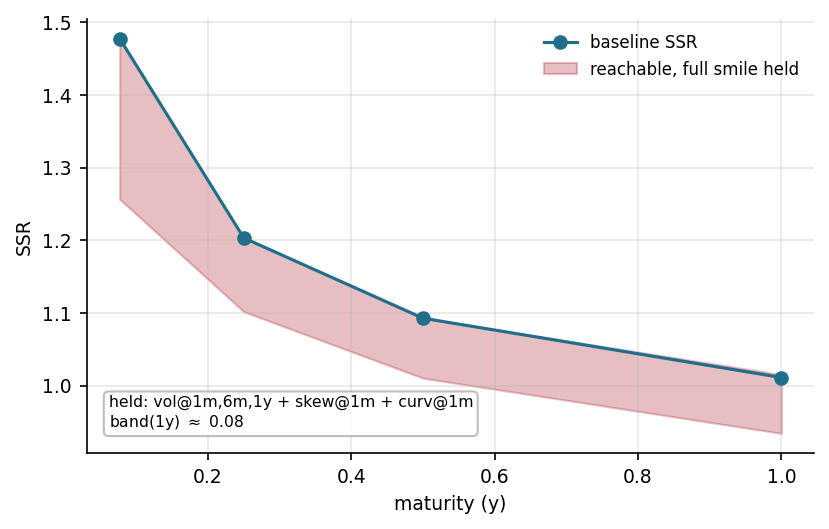
\includegraphics[width=0.62\textwidth]{figs/synthetic_main.png}
\caption{The statics/dynamics decoupling band at the shipped $2019$-$06$-$03$ fit, computed on the
construction of Section~\ref{sec:kernel}. Moving along the steepest static-preserving direction, the
SSR is confined to the shaded band; its long end spans $\approx1.54$--$1.59$ at fixed statics, a
width of $0.05$. The band widens sharply at the short end, where no observable is held.}
\label{fig:synth}
\end{figure}

\subsection{Data and calibration design}
\label{sec:realdata}

The real-data study calibrates one kernel per regime and reads it against two targets. Both
underlyings use the same design (Table~\ref{tab:design}); the one substantive difference is the
forward-variance block, risk-neutral on SPX and physical on NDX, which is the asymmetry the
off-index study has to overcome.

\begin{table}[htbp]
\centering
{\small
\begin{tabular}{lll}
\toprule
Component & SPX & NDX \\
\midrule
Static surface & SANOS on the selected date & SANOS on the selected date \\
Dynamic target & annual realised SSR panel & annual realised SSR panel \\
\quad residual weighting & uniform in tenor & inverse relative HAC error \\
Forward-variance target & selected-date VIX ATM-IV curve & realised constant-maturity var-of-var \\
\quad measure & $\mathbb Q$ (vol-index options) & $\mathbb P$ (own variance-swap strip) \\
\quad observation operator & readout and target coincide & corrected; \S\ref{sec:ndx} \\
\quad tenors fitted & all listed VIX expiries ($6$--$12$) & eight, $14$--$180$\,d \\
Model maturities & five SSR tenors, $1$wk--$3$m & same \\
Numerical resolution & single, fixed (Appendix~\ref{app:protocol}) & same \\
Optimisation & two-stage; accept on data cost & cold start \\
\bottomrule
\end{tabular}}
\caption{Calibration design. The forward-variance block differs in measure and in observation
operator, both handled explicitly in Section~\ref{sec:ndx}. The SSR residual weighting differs for a
measured reason: on SPX the fitted target and the estimator behind the reported error band agree to
$0.0\%$ at all nine dates, whereas one NDX date carries a $24.9\%$ split between them
(Appendix~\ref{app:data}), so off index the residuals are weighted by their own measured reliability.}
\label{tab:design}
\end{table}

\paragraph{The design constants.} Section~\ref{sec:identification} leaves the readout grids and
objective weights symbolic because they are choices of this study, not features of the model. Here
they are. The kernel of Section~\ref{sec:kernel} gives eight structural coefficients, ordered
$(\nu_{\mathsf F},\nu_{\mathsf S},\nu_{\mathsf L},\lambda_{\mathrm{skew}},
\rho_{\mathsf F},\rho_{\mathsf S},\kappa_{\mathsf F},\kappa_{\mathsf S})$, of which
$\rho_{\mathsf S}$ is pinned at zero, so the free dimension is $n_\theta=7$. The tenor grid is
$\mathcal{T}_{\mathcal{S}}=\{1,2,4,8,13\}\Delta t$ with $\Delta t=1/52$, so $d_{\mathcal{S}}=5$
spanning one week to three months. The forward-variance block runs from six to twelve on SPX,
according to how many VIX expiries survive the minimum-days filter, and is eight on NDX
($14$, $21$, $30$, $45$, $60$, $90$, $120$, $180$ days). The objective uses $w_{\mathrm{vov}}=0.8$
scaled by $\sqrt{d_{\mathcal S}/d_{\mathcal V}}$, so the two blocks carry comparable weight whatever
their lengths, with a ridge toward the stage anchor.

\paragraph{The counting condition is satisfied on both underlyings.} On SPX the data-bearing
residuals number $d_{\mathcal{S}}+d_{\mathcal{V}}=11$ to $17$ against seven free parameters; on NDX
they number $5+8=13$, the realised strip being trusted at eight tenors for the reasons given in
Section~\ref{sec:ndx} and Appendix~\ref{app:data}. The off-index fit is therefore over-determined
by six coordinates. That is an absence of underdetermination, not identification: it says the
readouts outnumber the free parameters, not that they pin them.

\paragraph{Fit quality is read against the target's own precision.} Each SSR target carries a joint
heteroskedasticity- and autocorrelation-consistent standard error (Appendix~\ref{app:hac}), HAC'd
across the regression slope and the skew denominator together since they are not independent. We
quote it as one number per year, the tenor-RMS of the relative standard error, and report each fit
against it. A residual smaller than that standard error is descriptive: it says the miss is small
relative to the target's estimated sampling variability, not that model and target have been shown
equal, and not that the residual could not have been smaller. The band is a \emph{reporting
benchmark}: nothing in the optimiser consults it, and it is not a stopping rule---the fits stop on
\texttt{xtol}, as Appendix~\ref{app:protocol} records. One row of Table~\ref{tab:crossregime} is an
exception to the reading above: at NDX $2017$ the fitted target is the Huber-robust $\beta$ while the
scale beside it is derived from the ordinary least-squares estimator, so for that row the number is a
precision scale from a different estimator, not that target's own standard error. With seven free parameters against five SSR tenors the kernel
can interpolate the point estimates outright, so the SSR block carries no positive residual degrees
of freedom and admits no in-sample specification test: agreement inside the band is necessary and
not sufficient. A test with positive degrees of freedom needs data withheld from the fit, which
Section~\ref{sec:heldout} does. Both underlyings are inside the band at every date in the panel.

All reported fits follow this protocol with no per-year tuning: one anchor, one schedule, one
resolution, for every date and both underlyings. The protocol, the numerical resolution and its
measured cost are in Appendix~\ref{app:protocol}; the realised-target construction and its four
corrections are in Appendix~\ref{app:data}.

\subsection{SPX: cross-regime identification}
\label{sec:spx}

\emph{Finding.} Across nine SPX regimes---the flattest term structure (2012), the COVID shock (2020),
the bear grind (2022), the steepest low-vol surface (2024)---the kernel reproduces the realised SSR
term structure \emph{inside the year's own sampling band at every date}, and fits the VIX ATM
implied-volatility curve to $1.8$--$9.2\%$ RMS. Each year is a single fixed calendar date, the first
June trading day.

\paragraph{Marginal compatibility.} The statics layer and the kernel are mutually consistent before
any dynamic target is imposed, and the part of that consistency which is structural should be
separated from the part which is measured. \emph{Structural.} The SANOS program is the joint linear
program of Appendix~\ref{app:sanoslp} over all expiries at once, whose calendar constraint
$U q_j \ge U q_{j-1}$ imposes convex order on the fitted marginals across ${\sim}20$ maturities to
${\sim}2.5$\,y. Continuum convex order is a \emph{standing guarantee supplied by the marginal
layer}, which this paper takes as a hypothesis rather than re-derives: the program enforces it as
call inequalities on a strike grid, so beyond the grid it rests on the smoothness of the mixture
basis (Appendix~\ref{app:sanoslp}).
The propagated kernel satisfies positivity and normalisation at every state and parameter value, and the martingale
lock~\eqref{eq:relock-state} at the numerical state the propagation carries, so the forward-start
return density has mass and forward equal to $1$ identically, not to within a tolerance.
\emph{Measured.} Two things hold only up to an error that is reported. The local-variance
\emph{level} is matched to leading order, its finite-step remainder~\eqref{eq:levremainder-prod}
sitting in Table~\ref{tab:realdata}. And exact propagation of the next spot marginal is the one
admissibility condition the production chain does not inherit, since the leverage overlay closes each
step by collocation rather than by the exact Gaussian identity~\eqref{eq:gm-closure}. What the chain
delivers is the finite-feature marginal compatibility of
Definition~\ref{def:eps-admissible}, and the condition it replaces is monitored rather than
assumed: $3$ call-bp and $26$ IV-bp out to six months, measured after the Gy\"ongy match of
Section~\ref{sec:fusion} and reported in Table~\ref{tab:realdata}. Those are discrepancies at the
quoted strikes, not a distance between laws, and no Wasserstein membership is claimed.

What the empirical sections below test is the part the construction does \emph{not} give for
free---the dynamics.

\paragraph{Dynamic fit.} The calibration is a two-stage protocol rather than a single optimisation:
a cold start, then a warm continuation from it with the calendar derivative $\partial_T C$ mollified
at source, accepting the second stage only where it lowers the data cost. It is deterministic,
reproducible on any new date, and never worse than the first stage by construction. Across the panel
it improves both blocks---the SSR half of the objective by $32.4\%$ and the forward-variance half by
$21.6\%$, for $23.3\%$ overall---and is accepted at four of nine dates ($2012$, $2016$, $2017$,
$2018$). It is the only intervention we tested that improves the forward-variance fit without paying
for it in the SSR block.

The resulting SSR RMS averages $1.70\%$ and is inside the target's joint-HAC standard error at all
nine dates, those bands running $5.1$--$16.4\%$; the VIX ATM RMS averages $5.14\%$
(Table~\ref{tab:crossregime}, term structures Figures~\ref{fig:ts-ssr}--\ref{fig:ts-vov}). Two
qualifications belong with those numbers. The acceptance test is \emph{in sample}---one bit per
date---and at two of the nine the margin is inside the objective's own staircase noise, so the choice
there is arbitrary, though those are also the dates where it costs least either way. And the
forward-variance instrument is \emph{biased}: the model's VIX law sits ${\approx}11.7\%$ low in
forward while the VIX smile slopes up at ${\approx}{+}0.6$ in $\log K$, so matching ATM volatility
identifies the vol-of-vol amplitude at a displaced point---a ${\approx}9.1\%$ systematic, pooled over
$88$ expiries, which is the same order as the entire forward-variance residual. A moneyness-matched
correction was constructed and \emph{rejected}: the displacement depends on $\bth$, so lowering the
amplitude and raising the forward are substitutes, and the correction opened a flat direction rather
than closing a bias (Appendix~\ref{app:data}). The amplitude is therefore identified to within about
ten percent, and we report it as such.

\paragraph{External calibration of the level.} A published estimate places the empirical SPX
skew-stickiness ratio between $0.9$ and $2.0$ over $2012$--$2022$, at maturities from one month
outwards and on a $60$-day rolling window~\cite{abijaber2025}. Over that maturity range the realised
targets used here sit inside it at every tenor and every year ($1.15$--$1.93$ from one to three
months); the fitted model leaves it once, at $2.03$ at one month; the one-week targets run higher,
$1.28$--$2.46$, at a maturity the published band does not cover.

That comparison anchors the level rather than bounding the variation. The skew-stickiness ratio is
an instantaneous ratio of covariations, so it is never observed, only estimated, and the width of any
reported interval mixes market variation with the variance of the estimator behind it: the HAC
standard errors of Appendix~\ref{app:hac} run $4$--$18\%$ of the target on the annual window used
here, hence roughly twice that on a sixty-day one, so a \emph{constant} ratio of $1.4$ read through
such an estimator would print about $[0.96,1.84]$ at two standard errors---nearly the published
interval itself.

The more informative comparison is not the level but whether fitting the smile delivers the
dynamics. It does not. A two-factor Bergomi calibrated to the same smile does not reproduce the
skew-stickiness term structure, and the two-factor Quintic OU---a model built to target smile
dynamics---reaches the market range only once an SSR constraint is imposed \emph{alongside} the
smile~\cite{abijaber2025}---consistent with the inverse-problem argument of
Section~\ref{sec:intro}: skew-stickiness enters the observed range only when it is explicitly
constrained.

\paragraph{Stability across dates and optimizer basins.} Three checks, reported in full in
Appendix~\ref{app:protocol}. The joint objective is \emph{loosely identified}: a cold start
and a warm continuation from a neighbouring fit can differ by up to ${\sim}0.6$ points of SSR RMS,
comparable to the fit quality being reported. That freedom is bounded and measured: across four
sensible seeds the total data cost spans $0.06\%$, the cold start best among them, while a seed
taken from a different tenor set lands one date $41\%$ worse---which is why the protocol fixes the
seed rather than searching over seeds. The parameters vary more than their fitted readouts do: any
two fits the protocol accepts reproduce the same SSR and skew term structures to within the reported
RMS, the residual freedom lying in the $\bth$-directions those readouts leave soft
(Table~\ref{tab:jac7}). Section~\ref{sec:discussion} draws the consequence. This is the decoupling of
Section~\ref{sec:decouple} seen from the calibration side, and it is why the object carried
downstream is the readout rather than
$\bth$. Repeating the calibration at three static dates per year over $2012$--$2024$ moves the
fitted SSR term structure by a median $7.4\%$ at one week and $2.6$--$4.0\%$ from one to three
months, inside the realised-SSR sampling band the fit is judged against. And the statics/dynamics
decoupling holds regime-independently \emph{in the variance}: with the digital band given zero
weight, so the kernel is fit to the dynamics alone, the from-spot leveraged marginal still matches
the SANOS marginals to ${\approx}5\%$ survival RMS in calm, high-vol and grind alike---the leverage
carries the variance level
whatever the dynamics do. The digital band reads survival probabilities, which are integrals of
the density and nearly insensitive to an at-the-money slope,
and the propagated skew does fall short of the target marginal's---$48\%$ of it at one week rising
to $72\%$ at three months, on the same inversion at both sides. That is a property of the overlay
rather than of the fit, since a variance rescaling constrains no third moment, and it does not enter
the SSR readout, which normalises by the model's own skew.

\emph{Boundary.} The two target blocks sit on different clocks---the SSR is an annual $\mathbb P$
regression while the marginal engine and the VIX curve are same-date $\mathbb Q$
cross-sections---and the static-date experiment above measures the cost of that pairing.

\begin{table}[htbp]
\centering
{\small
\begin{tabular}{lcc}
\toprule
Diagnostic & Result (real SPX) & Target \\
\midrule
Marginal discrepancy, $\mu_j\cK_j$ vs.\ $\mu_{j+1}$ & $3$ call-bp / $26$ IV-bp (${\le}6$\,m) & within bid--ask \\
Leverage remainder $\delta_{\mathrm{LV}}$~\eqref{eq:levremainder-prod} & $0.40$--$3.19\%$ weighted RMS & leading-order match \\
Forward-start density & mass, forward $=1$ to machine $\varepsilon$ & exact \\
Forward-start skew & rolls down $-0.5\to-0.14$ & flatter than spot \\
From-spot marginal, dynamics-only fit & ${\approx}5\%$ survival RMS & all regimes \\
Second-order leverage $\E[\nu\mid z{=}0]$ & $\approx0.7$; from-spot ATM ${+}10\%$ & --- \\
\bottomrule
\end{tabular}}
\caption{Architecture-level diagnostics on real SPX chains: what holds before and after the dynamic
fit, independently of the per-year fit errors of Table~\ref{tab:crossregime}. The marginal row is
measured \emph{after} the structural Gy\"ongy match, and is the finite-feature discrepancy of
Definition~\ref{def:eps-admissible} at the quoted strikes, not a distance between laws. The
leverage row is
$\delta_{\mathrm{LV}}=\Var_{\cK^{L}}(\Delta Z\mid c,z)/\bigl(L^2\overline V_c\bigr)-1$
of~\eqref{eq:levremainder-prod}, with both moments over the joint $(k,\ell)$ factor-node/branch law,
evaluated at the nodes the production step visits and weighted by the production weights, so it is a
probability-weighted summary rather than a maximum over tail nodes; ranges are across the nine
shipped fits.}
\label{tab:realdata}
\end{table}

\begin{figure}[htbp]
\centering
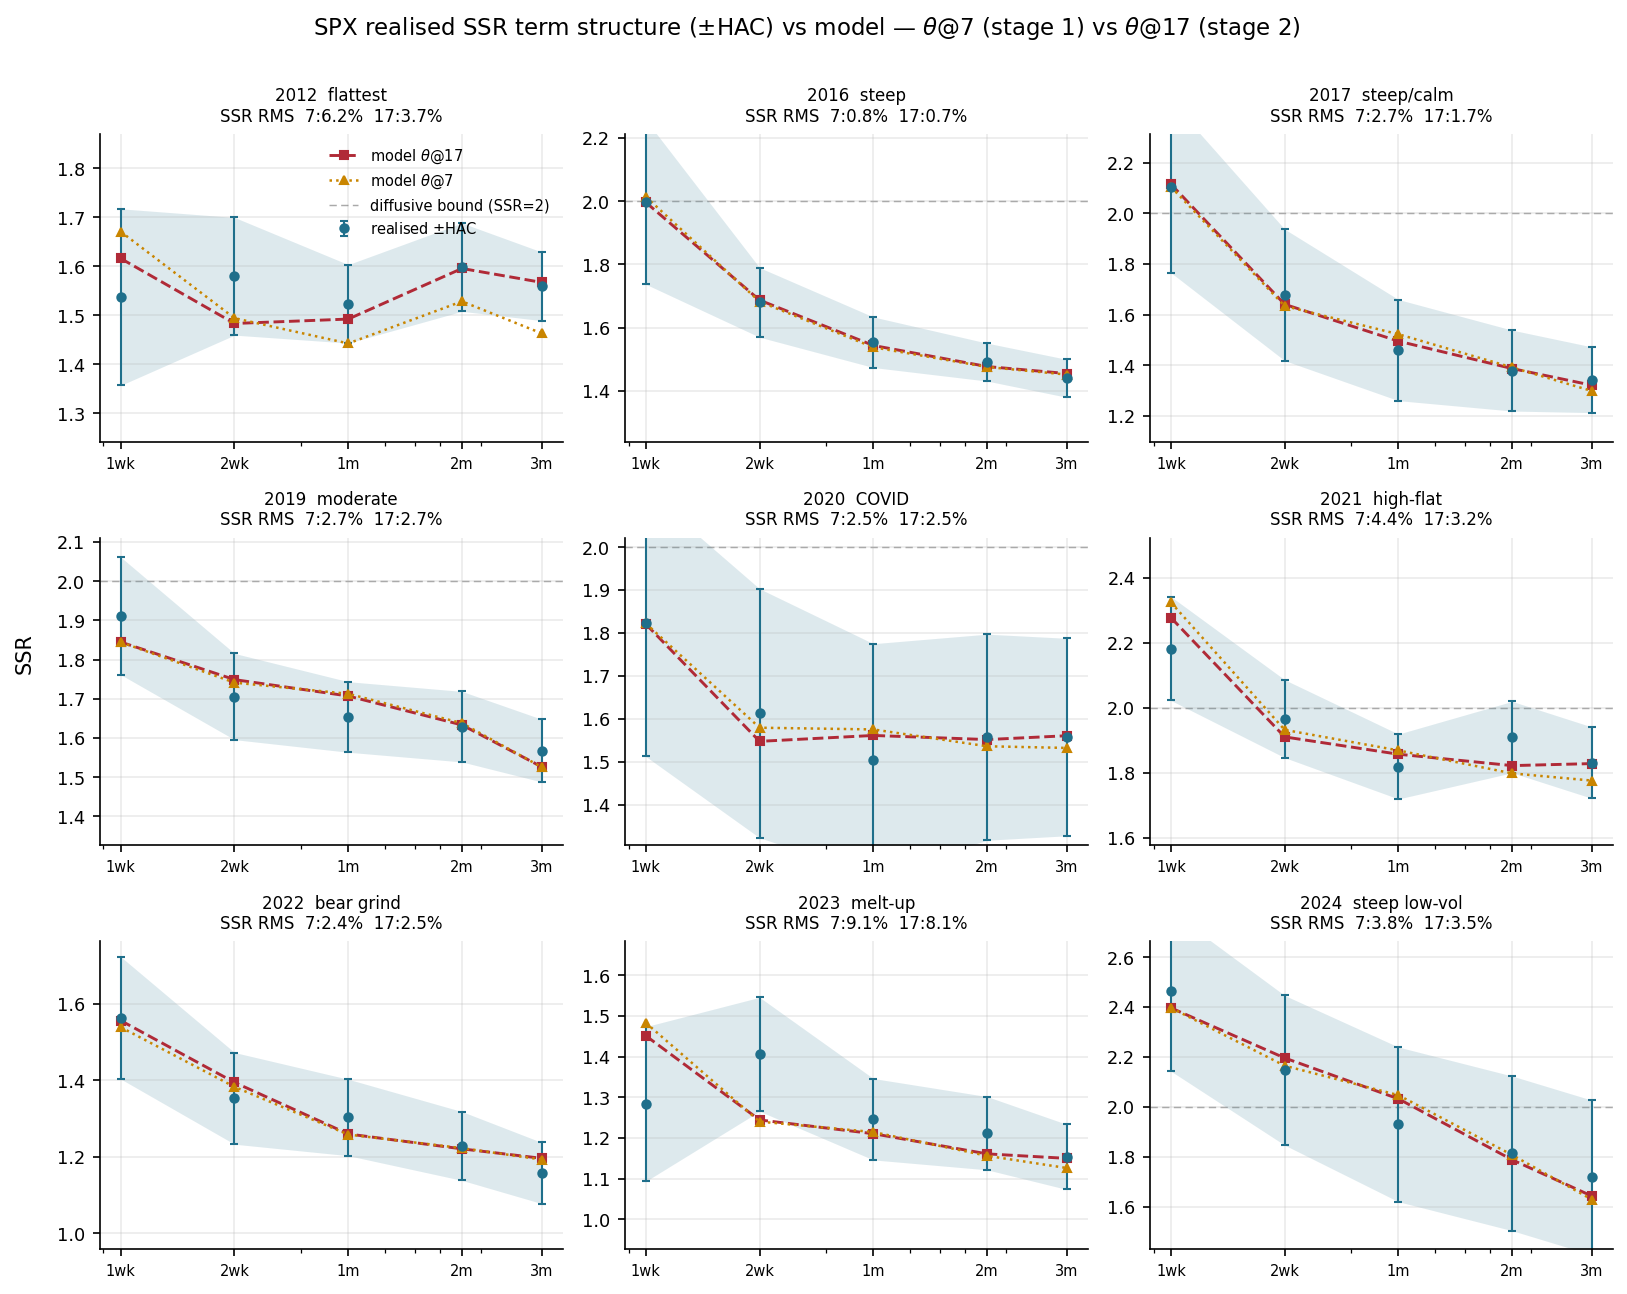
\includegraphics[width=\textwidth]{figs/real_ssr_ts.png}
\caption{Realised SSR term structure vs.\ model, one date per year, $2012$--$2024$. Markers, error
bars and shaded band: the realised skew-stickiness (a calendar-year $\mathbb P$ regression) with its
joint Newey--West HAC $\pm1$\,SE, HAC'd across the regression slope and the skew denominator together
since they are not independent (Appendix~\ref{app:hac}). Dashed: the model SSR at the fitted $\bth$,
from the two-stage protocol of Section~\ref{sec:spx}. Plain dashed line: the diffusive
$H{=}\tfrac12$ short-time limit $\SSR\to2$, a continuous-time benchmark rather than a bound on the
finite-step statistic. \textbf{The model sits inside the band at every tenor of every date}; each
panel quotes that year's RMS against its displayed precision scale, which on SPX is the target's
joint-HAC standard error throughout.}
\label{fig:ts-ssr}
\end{figure}

\begin{figure}[htbp]
\centering
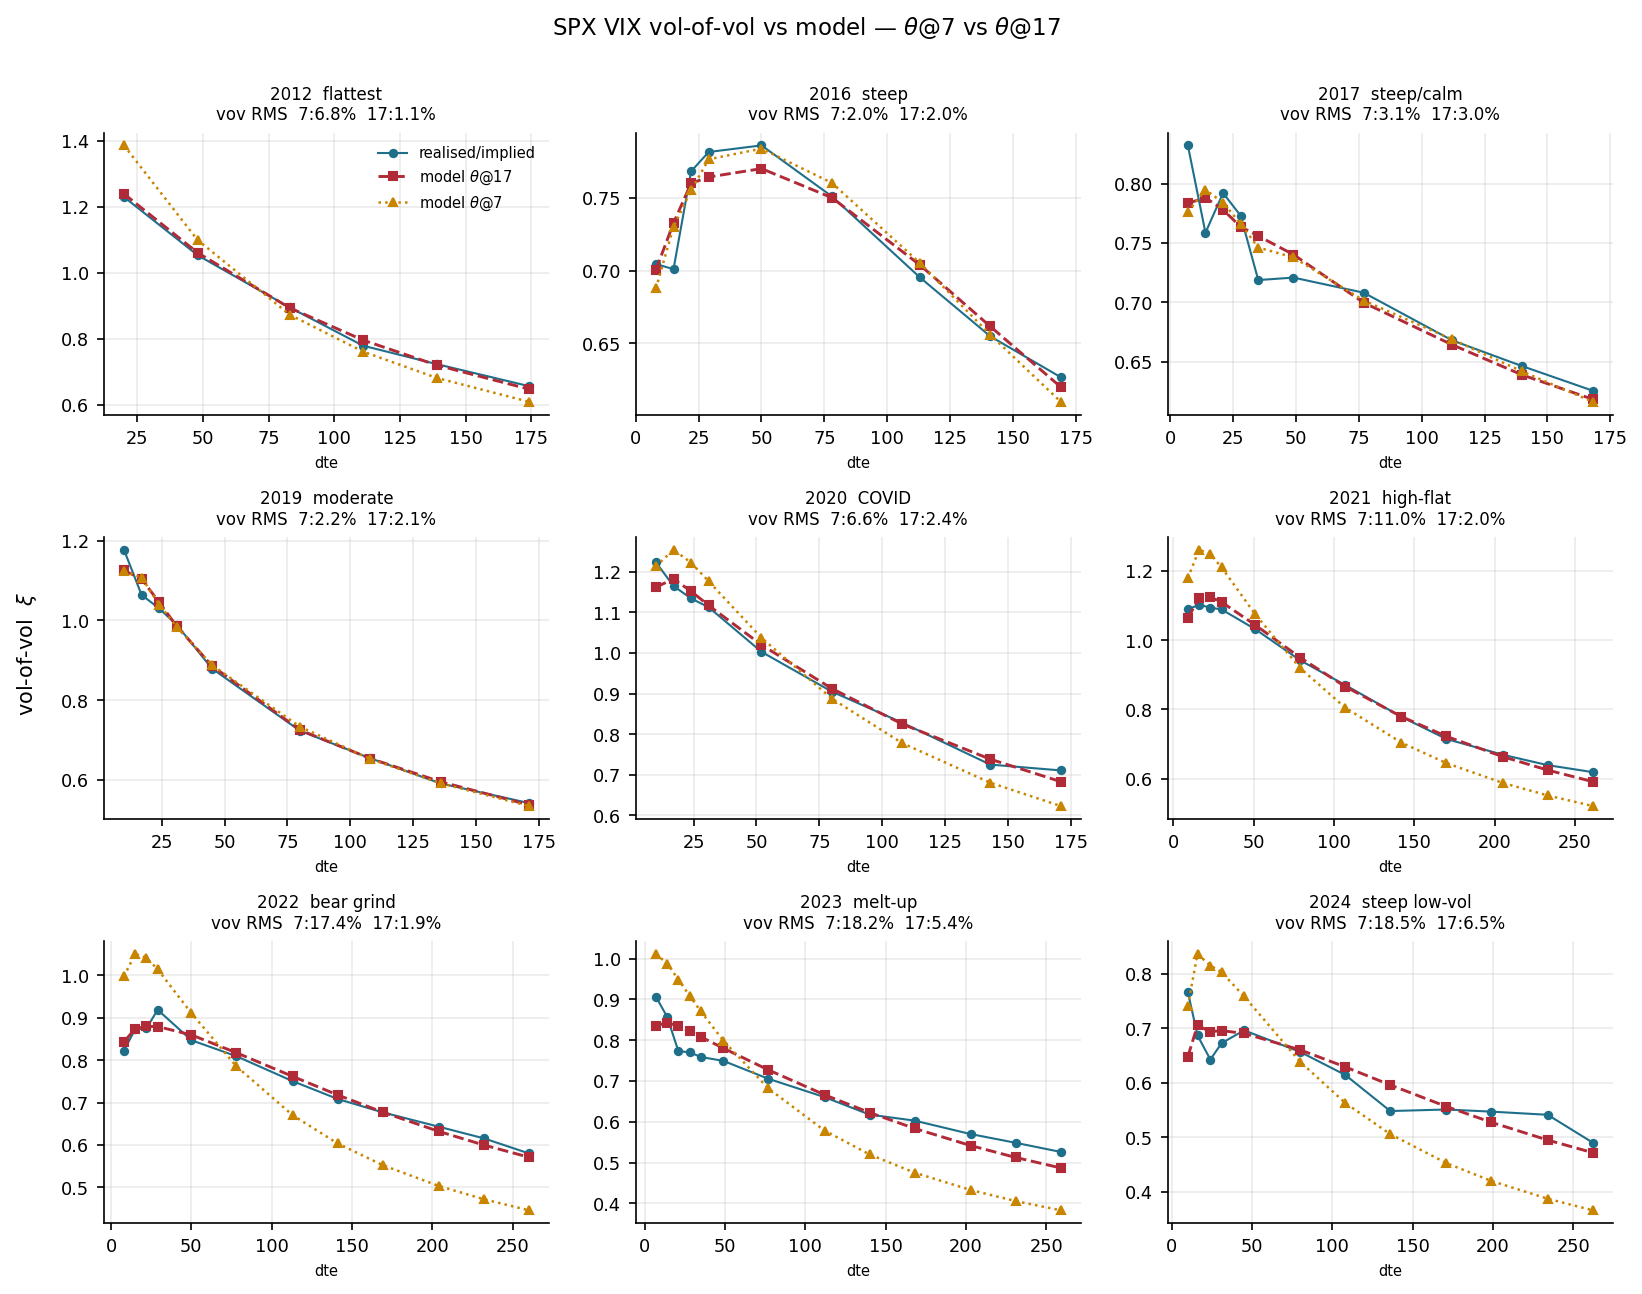
\includegraphics[width=\textwidth]{figs/real_vov_ts.png}
\caption{VIX ATM implied volatility term structure vs.\ model, same dates. Markers: the VIX-implied
ATM volatility $\xi$ at every listed VIX-option maturity surviving the minimum-days filter---six at
$2012$, twelve by $2021$, so the fit is asked for more where the market provides more---a
\emph{single-day} $\mathbb Q$ read carrying no sampling band. Dashed: model. On this underlying the
readout and the target are the same object, so no observation-operator correction is involved; the
amplitude is however identified only to within the ${\approx}9.1\%$ instrument bias of
Section~\ref{sec:spx}.}
\label{fig:ts-vov}
\end{figure}

\subsection{Held-out tenors: what the SSR block actually determines}
\label{sec:heldout}

\emph{Finding.} The long end of the skew-stickiness curve is implied by the rest of the calibration;
the short end is fitted. Withholding the two interior tenors costs a median $2.95\%$ on the unseen
points, below the target's own estimated standard error at eight of nine dates. Withholding the two
\emph{end} tenors costs a median $8.72\%$, and the damage is entirely at one week.

\emph{Design.} Section~\ref{sec:realdata} leaves the SSR block with no residual degrees of freedom;
these create some. Tenors are dropped from the objective by zeroing their entries in the residual
weight vector, the survivors renormalised so the retained block keeps its scale against the
forward-variance block, and the model then scored where it was not told the answer. Everything
else---protocol, seed, box, ridge, forward-variance targets---is the shipped configuration.

\begin{table}[htbp]
\centering{\small
\begin{tabular}{lcccccc}
\toprule
& \multicolumn{2}{c}{interior: fit $1$wk/$1$m/$3$m} & \multicolumn{2}{c}{ends: fit $2$wk/$1$m/$2$m} & \\
\cmidrule(lr){2-3}\cmidrule(lr){4-5}
Year & held RMS & $2$wk\ \ \ $2$m & held RMS & $1$wk\ \ \ $3$m & target s.e. \\
\midrule
2012 & $2.95$ & $-1.7$\ \ $-3.8$ & $3.97$ & $-4.8$\ \ $-3.0$ & $7.0$ \\
2016 & $\mathbf{47.78}$ & $\mathbf{+67.6}$\ \ $-0.7$ & $8.72$ & $-10.3$\ \ $-6.9$ & $5.1$ \\
2017 & $1.31$ & $-0.1$\ \ $-1.9$ & $3.66$ & $-2.9$\ \ $+4.3$ & $11.9$ \\
2018 & $5.09$ & $-6.7$\ \ $+2.7$ & $12.10$ & $+17.1$\ \ $+0.6$ & $10.6$ \\
2019 & $2.52$ & $+3.3$\ \ $-1.2$ & $9.61$ & $-13.6$\ \ $-0.2$ & $5.2$ \\
2020 & $0.94$ & $-0.4$\ \ $-1.3$ & $13.42$ & $-12.8$\ \ $-14.0$ & $16.4$ \\
2021 & $2.72$ & $-1.2$\ \ $-3.7$ & $2.24$ & $+3.0$\ \ $+1.2$ & $5.7$ \\
2022 & $3.51$ & $+3.2$\ \ $+3.8$ & $20.45$ & $-28.3$\ \ $-5.8$ & $6.0$ \\
2024 & $2.98$ & $+3.8$\ \ $-1.9$ & $7.80$ & $-11.0$\ \ $+0.2$ & $14.7$ \\
\midrule
median & $2.95$ & & $8.72$ & & \\
inside s.e. & $8/9$ & & $5/9$ & & \\
\bottomrule
\end{tabular}}
\caption{Held-out SSR tenors, nine SPX dates. \emph{held RMS} is over the two withheld tenors only;
the per-tenor columns are signed relative errors in percent. \emph{target s.e.} is that year's
joint-HAC standard error (Appendix~\ref{app:hac}), an estimate of the target's sampling
variability.
Excluding $2016$ the interior held-out RMS runs $0.94$--$5.09\%$.}
\label{tab:heldout}
\end{table}

\emph{The two ends behave differently.} Splitting the ends experiment by
tenor, the three-month error has median magnitude $3.0\%$ and no sign preference ($5/9$ negative),
while the one-week error has median magnitude $11.0\%$ and is negative at seven of nine dates---a
systematic undershoot, not noise. Predicting the long end from the interior tenors and the
forward-variance curve works about as well as interpolating; predicting the short end does not. The
model reaches the realised one-week value when that value is in the objective, and does not get
there on its own.

Two independent results point the same way. The identifiability spectrum
(Table~\ref{tab:jac7}) makes the slow persistence $\kappa_{\mathsf S}$ the stiffest direction in the
problem and the fast return correlation $\rho_{\mathsf F}$ the softest; and the diffusive short end is the first limitation listed in
Section~\ref{sec:discussion}. What the held-out test adds is a magnitude and a direction for a
limitation that was previously asserted.

\emph{The $2016$ interior failure is a shape failure, not a numerical one.} With the two-week tenor
withheld the model places it at $2.80$ against a realised $1.67$, between a well-fitted one-week
($1.98$) and one-month ($1.60$)---a hump no monotone decay would produce. It is not a numerical
artefact of the ratio: \eqref{eq:exactssr} normalises by the model's own average skew and so
diverges as that approaches zero, but the $2016$ fit sits at $0.39$, inside the $0.24$--$1.16$ the
panel spans and well clear of the $0.10$ at which a parameter scan finds the readout diverging. That
margin is recorded per fit, which is what verifies the nondegeneracy hypothesis of
Proposition~\ref{prop:readout} at the vectors the calibration visits.

\emph{Boundary.} Both designs withhold tenors within a date, not dates. The forward-variance block is
fully fitted throughout, the static surface is the same date's, and the withheld and retained SSR
targets come from one panel of daily returns and are therefore correlated. This tests what determines
the \emph{shape} of the SSR term structure; it is not out-of-time validation, and the annual target
window of Section~\ref{sec:realdata} is untouched by it.

\subsection{NDX: portability, and what the off-index target actually measures}
\label{sec:ndx}

\emph{Finding.} The model travels off SPX using no volatility-index data of the underlying's
own---the targets are its own option strip and realised increments---though the
observation-operator correction those targets need is \emph{estimated on SPX and transported}, which
is the one imported ingredient and is quantified below. It travels on \emph{both} blocks: the SSR RMS is $1.92\%$---inside the target's estimation band at all nine dates, and
numerically close to SPX's $1.70\%$ on a target built from NDX's own strip, though a residual
inside one estimated standard error is a descriptive comparison and not a test---and the
eight-tenor realised variance-of-variance is fitted to $14.3\%$ against a target carrying $24\%$ of
its own roughness. The steep-decay shape gap that a nearest-expiry realised target produces is
substantially an \emph{observation-operator} artefact rather than a limit of the two-timescale decay.

\emph{The observation operator.} The model's forward-variance readout~\eqref{eq:vixatm} prices an
option expiring at $\tau$ on a \emph{$30$-day} forward variance: the variance window is fixed and
$\tau$ varies. On SPX the target is that same object. Off index the target must
be~\eqref{eq:ndxvov}, the realised volatility of the \emph{$T$-day} variance-swap level, and the two
are not counterparts. The gap is quantifiable on SPX, the one underlying carrying both sides, where
the ratio is smooth and monotone in
tenor, from $0.33$ at one week through unity near three months to $1.22$ at six months, with nine to
ten years of coverage at every tenor. Uncorrected it is large enough to dominate: it makes the
realised term structure appear to decay faster than a mean-reverting kernel can represent, and the
demanded decay exponent falls from $0.44$ to $0.18$ once it is applied---from outside the model's
reach to comfortably inside. The supporting diagnostic is that \emph{SPX inherits the same apparent
ceiling when fed realised targets}, which points at the target construction rather than at the
off-index kernel without ruling the latter out.

\emph{Four corrections, two checked on held-out tenors.} The realised series needs a constant-maturity
construction (the nearest-expiry series rolls, and a realised volatility of a rolling series counts
each roll as a move); a physical validity bound (of $25{,}576$ observations exactly one lies outside
the range an index variance-swap level can occupy, and its single increment carried $92.5\%$ of that
cell's annual variance); removal of increments spanning a bracketing-expiry change beyond three
months, where listed expiries are sparse enough that the switch is a genuine discontinuity; and the
observation-operator correction above. Two were checked on tenors withheld from the fit. Fitting
only the $30$- and $90$-day anchors and scoring the seven withheld tenors, each target favours the
run trained on it: the corrected-target run wins by a mean $32.5\%$ at nine of nine dates when
scored against the corrected series, and the raw-target run wins by a mean $15.2\%$ at seven of nine
when scored against the raw one. The correction is supported because the first margin exceeds the
second, not because either scoring is neutral. The held-out-tenor RMS is large in absolute terms
either way---$31$--$46\%$ across the four combinations---so this ranks two targets rather than
validating a level. Fitting only $14$--$45$ days, the churn removal predicts the
held-out $60$--$180$ day range $21.7\%$ better---while dropping the \emph{same number} of increments
at random improves it by $0.3\%$, so the gain is attributable to those increments specifically and
not to thinning a noisy series. Details, and two statistical screens that were built and rejected on
their own pre-specified diagnostics, are in Appendix~\ref{app:data}.

\emph{What the remaining residual co-moves with.} Measured as each year's
deviation from its own power law---a shape the estimator has no reason to violate---the realised term
structure carries $24\%$ RMS of roughness against the model's $4.8\%$, a factor of five. Across the
nine dates the fit residual and that roughness correlate at $R^2=0.93$ with an intercept near $4\%$:
the cross-year variation in fit quality moves with the target's own smoothness. The
daily coherence of the strip also degrades across the sample---the first principal component of the
eight-tenor increment panel explains $96\%$ of variance in $2012$ and $46\%$ by $2020$---which is
itself a reason off-index calibration is harder than the index case. Nothing here shows the
off-index dynamics to be the same as SPX's; what it shows is that the instrument is measurably
noisier, which is consistent with the residual gap without establishing it.

\emph{What does not dissolve.} One deficiency survives every correction, and it is visible on SPX
rather than NDX. Measuring each series against its own log-log shape, the model undershoots the
forward-variance readout at approximately six weeks by $4.0\%$ on SPX ($t=3.6$ across the panel),
against a traded VIX option price with no correction, transport or estimator between model and
observation. The same tenor carries the largest residual on NDX ($+19.6\%$), amplified roughly
fivefold by the noisier instrument; the residual's \emph{shape} is common to the two underlyings
(correlation $+0.82$) while its amplitude is not. We report this as a bounded limitation of the
two-timescale decay rather than repair it.

\emph{Boundary.} The correction cannot be verified where it is applied, so
Appendix~\ref{app:data} tests it on held-out tenors instead. The SPX control bears on it in both
directions: the residual oscillation is present on SPX too, so it is not purely a transport
artefact, but it is $4.4$ times larger off index. Separately, the off-index marginal is modestly
fat-tailed relative to the data (${\sim}2$--$3\times$ the excess kurtosis), a discretisation feature.

\begin{figure}[htbp]
\centering

\includegraphics[width=0.92\textwidth]{figs/ndx_summary.png}
\caption{Off-SPX (NDX), both channels in one view, nine years. Filled circles: the realised-SSR fit
RMS. Shaded bars: that year's displayed precision scale---the target's joint Newey--West HAC
standard error, except at $2017$, whose target is the Huber-robust $\beta$ while the scale shown is
OLS-derived (marked $\dagger$ in Table~\ref{tab:crossregime}). Either way it is a scale to read the
residual against, not a bound the residual could not fall below. Open squares: the variance-of-variance fit RMS, a realised target carrying no band of
its own. Dashed line: that target's measured roughness---its RMS deviation from its own power law,
$24\%$. That is how far the target departs from its own smooth shape---\emph{roughness}, not a
standard error and not a noise bound---so it carries none of the sampling interpretation the SSR band
does, and the line is the \emph{panel-average} roughness rather than each date's own.
\textbf{Every SSR residual sits inside its band.}}
\label{fig:ndx-summary}
\end{figure}

\subsection{What the calibrated kernel says about smile motion}
\label{sec:smilemotion}

\emph{Finding.} The calibrated kernel places SPX on the sticky map in two independent coordinates:
the smile's \emph{level} rides with spot at the SSR, while its \emph{shape} is very nearly frozen in
moneyness.

\emph{Evidence.} Taking the same exact-$\beta$ readout across the whole at-the-money neighbourhood
rather than at the level alone (Figure~\ref{fig:dynamics}), the level responds as
$\partial_{\ln S}\sigma_{\mathrm{ATM}}=\SSR\,\mathcal S$ with $\SSR$ running from $1.89$ at one week
down to $1.57$ at three months---far from sticky-moneyness ($\SSR{=}0$), between sticky-strike ($1$)
and the local-volatility limit ($2$), and on the Doeff--Kamal $H{+}\tfrac32$ backbone through the
belly. The skew's own response $\partial_{\ln S}\mathcal S$, normalised by the rate at which a
strike-pinned smile would swing it (twice the curvature), runs from $0.001$ at one week to $0.03$ at
three months: the shape is essentially frozen in moneyness, with a small and realistic steepening on
sell-offs that grows mildly with tenor. The one-month
smile shifts up nearly in parallel on a $1\%$ drop, unlike the flat sticky-moneyness or the tilted
sticky-strike responses.

\emph{Interpretation.} The textbook equity picture comes out as a result rather than an
assumption: the fitted kernel holds the shape sticky and lets only the level ride, so the smile's
whole response to a spot move collapses to the single number~\eqref{eq:ssr-delta} folds into a
delta.

\emph{Boundary.} The frozen shape is a structural constraint as much as an empirical match: under
the translation invariance of Section~\ref{sec:kernel} the conditional smile is a function of the
volatility regime alone, so shape responds to spot only through the leverage-induced regime shift.
A \emph{deterministic, spot-level-dependent} shape lies outside the model's reach.

\begin{figure}[htbp]
\centering
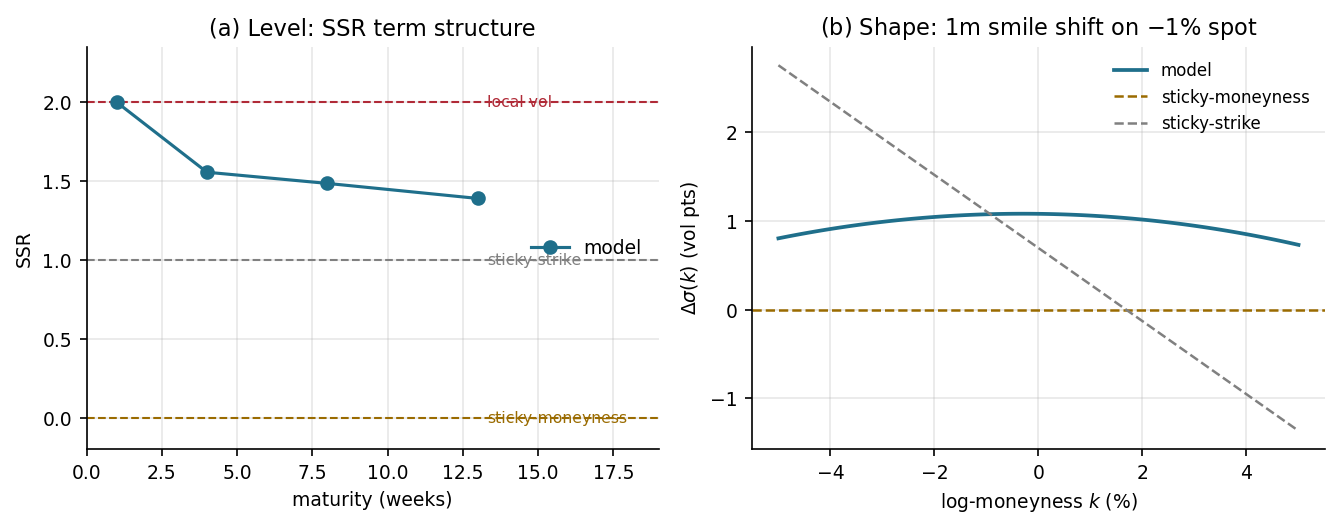
\includegraphics[width=\textwidth]{figs/real_dynamics.png}
\caption{Where the calibrated model sits on the sticky map (SPX, conditional-smile response to a spot
move, by moment). \textbf{(a)}~\emph{Level}: the SSR term structure, running $1.89$ at one week to
$1.57$ at three months, between the sticky-strike and local-volatility reference lines. \textbf{(b)}~\emph{Shape}: the one-month smile's
response to a $-1\%$ move, against the sticky-moneyness and sticky-strike references. The level rides
and the shape does not.}
\label{fig:dynamics}
\end{figure}

\section{Synthesis, limits, and conclusion}
\label{sec:discussion}

\subsection{What is identified}

Fixing the marginals does not fix the dynamics. With five smile observables held to a few basis
points, the long-end skew-stickiness still moves across a band of width $0.05$ around the calibrated
fit: the gap European prices leave open is small enough to be a calibration target and large enough
to matter.

Fitting the two calibrated blocks narrows the kernel: across the nine-regime panel the SSR residual
RMS lies below the tenor-RMS estimated standard error at every date, and the forward-variance
residuals---whose target carries no sampling band---are reported separately
(Section~\ref{sec:spx}). But not uniquely: distinct
parameter vectors reproduce the same readouts along the soft directions Table~\ref{tab:jac7}
locates, median effective rank five of seven.

What the procedure identifies is therefore the tolerance set~\eqref{eq:tolset}, a neighbourhood of
the exact class~\eqref{eq:readout-equiv}, with the block-specific tolerances
of~\eqref{eq:tolset}. The parameter vector is loose---two accepted fits can differ by about a point
of skew-stickiness RMS---while the readout it produces is stable under both perturbations that
matter, the static date it is calibrated on and the sample it is used out of. The readout is what is
carried downstream.

Read as a contract, that states what may and may not be claimed. Only outputs that are themselves
functionals of the selected readouts inherit the identification; other prices are model-implied.
The distinction bites precisely where it is tempting to ignore it: a forward-starting or
path-dependent structure is identified in this sense only to the extent that its value depends on
the joint law through the first-order spot--vol response and the forward-variance amplitude, and
such prices can also depend on joint tails and on higher-order features $\Rcal$ never sees. Two
failures of identification then have different remedies. \emph{Within} the readout set are
directions $\Rcal$ leaves soft, which Table~\ref{tab:jac7} locates and which sharper targets of the
same kind would tighten. \emph{Outside} it, statistics no chosen readout sees are not weakly
identified but unconstrained: the Zumbach effect and the broader time-reversal asymmetry of
volatility, any asymmetry in the vol-of-vol itself, and the joint tail behaviour of spot and
variance---\cite{abijaber2025} shows the question is live by testing the Zumbach effect
explicitly.

\subsection{What the two-timescale realization captures}

Classical stochastic-local volatility also matches vanilla marginals and also produces smile
dynamics; the distinction is which quantities are \emph{independently imposed}. There the residual
spot--vol response falls to the backbone, which is why calibrated backbones are documented to
cluster~\cite{bergomi2017}; here the overlay carries the marginal level, leaving the
innovation leverages and the two persistence loadings free to be identified against an observed
term structure.

Four features make the identification computable: the transition law is \emph{explicit}, so prices,
Greeks and readouts are deterministic fixed-resolution evaluations rather than
particle~\cite{guyonhl2012} or grid computations; the martingale
property is enforced \emph{structurally}, by the branch law, not by penalty; the fast/slow split
gives the spot--vol response a term structure with two interpretable timescales rather than a single
decay; and return--regime dependence runs through a shared branch index, coupling leverage and
variance dynamics inside the kernel rather than afterwards. Propagation stays in the finite-mixture
class throughout, which is what keeps the whole chain deterministic. Against frontier
stochastic-local volatility---multi-factor, rough, or neural---the edge is this combination, not
dynamic control as such.

\subsection{Limits revealed by the evidence}

Four limitations survive the empirical study, each exposed by specific evidence and each pointing at
a different kind of extension (Table~\ref{tab:limits}). The short end is the weak part of the fit,
and the held-out test of Section~\ref{sec:heldout} measures how weak: withhold the one-week tenor
and the model undershoots it by a median $11\%$, at seven of nine dates, while the withheld
three-month tenor is recovered to $3\%$. The model skew-stickiness also rises to the
$H{=}\tfrac12$ ceiling $2$ where SPX prints ${\approx}1.5$ sub-month; the conditional smile shape is
near-frozen in moneyness, responding to spot only through the regime channel; in the off-index
steep-decay years the realised variance-of-variance falls from $30$ to $90$ days at a ratio
${\approx}0.4$ against the kernel's floor ${\approx}0.58$; and observationally equivalent parameter
vectors populate the soft Jacobian directions. None is a numerical defect.

\begin{table}[htbp]
\centering
{\small
\begin{tabular}{>{\raggedright\arraybackslash}p{0.42\textwidth} >{\raggedright\arraybackslash}p{0.42\textwidth}}
\toprule
Limitation & Natural extension \\
\midrule
Diffusive short end & rough or multiscale kernel ($\SSR\to H{+}\tfrac32$)~\cite{fukasawa2026} \\[2pt]
Spot-level-independent conditional shape & state-dependent mixture weights \\[2pt]
Two-timescale decay floor & richer persistence spectrum \\[2pt]
Weak parameter identification & forward-start skew and variance-index smile data \\
\bottomrule
\end{tabular}}
\caption{Limitations as a research map. The first two are consequences of the construction---the
translation invariance that makes the readouts exact closed forms is what freezes the conditional
shape---the third is a property of the two-factor family, and the fourth of the data available to
identify it.}
\label{tab:limits}
\end{table}

One thing the evidence does \emph{not} establish is a hedging edge. What is measured is a
\emph{smile-roll residual variance}: the mean square of
$\Delta\sigma_{\mathrm{ATM}}-R\,s\,r$ over each window---the part of the at-the-money move that a
one-parameter delta family $\Delta_{\mathrm{BS}}+\mathrm{Vega}\,R\,\mathcal S/S$ leaves
behind---with $s$ the strike slope and $r$ the return. It is a proxy for hedging error, not a traded
profit and loss: no vega weighting, no position, no transaction cost. On that proxy the family is
worth a great deal against no adjustment---$R{=}0$ carries $2.8$--$3.4\times$ the residual variance
of the industry minimum-variance delta---and nothing against a competent choice of $R$. Out of
sample on $2015$--$2023$, under the same train-only affine procedure, fitted separately to each
competitor, and a $20$-row purge between train and test---the map is fitted on $21$-day forward
outcomes, so without an embargo the last training rows would look into the first test
origins---the calibrated kernel's own one-month readout, the corrected constant leg (the $R{=}1.5$
input mapped to the training-sample target mean), an analytic smile-implied $R$ and a trailing
at-the-money regression are all within
$5\%$ of the cross-strike Hull--White delta of~\cite{hullwhite2017} and of each other. The kernel leg
is served under a strict lag: each annual fit is calibrated to that calendar year's realised SSR, so
on any date in year $Y$ the forecaster uses the most recent fit from a year strictly before $Y$,
never the contemporaneous one. The
minimum-variance delta collapses to estimating one number, and one number is estimable many ways,
so the model's dynamic content has nowhere to show up. Where it should show up instead is in
quantities the marginals cannot price at all---forward-start and path-dependent structures, whose
very definition needs the forward implied volatility the marginals leave
open~\cite{glasserman2010forward}, and for which the construction supplies deterministic
finite-sum forward densities. That comparison is left to future work.

Two limitations deserve a word. The value $2$ is the short-time limit of the skew-stickiness under a
diffusion, not a bound on the finite-step statistic: where the realised one-week value exceeds
it---as it does in the lowest-vol years, at ${\approx}2.1$--$2.5$---the kernel follows it there. And
the off-index residual combines the two-factor decay floor with the physical measure in which that
target must be quoted; the two cannot be separated with the data available there.

\subsection{What would sharpen the identification}

What would sharpen the identification is data, not a larger parameter count. The variance-index
\emph{smile}---its skew and tails, not only the at-the-money level---reads the vol-of-vol shape under
$\mathbb Q$, and the atomic variance-index law of Section~\ref{sec:fwdvar} prices it across strikes with
no new machinery; the forward-start smile skew would supersede the realised proxy used here as the
clean risk-neutral observable of spot--vol leverage, but it needs cliquet quotes absent from listed
feeds. The framework may also be adapted to intraday surfaces, but jumps, seasonal liquidity, pinning
and synchronized quote construction require a separate model and dataset~\cite{bandi2026}.

Two directions of extension follow from the architecture rather than from this instance of it: the
contribution is the architecture, not the two-factor kernel that
occupies the framework here.

\emph{Refining the topology.} Enlarging $\Rcal_{\mathrm{cal}}$ shrinks
both~\eqref{eq:readout-equiv} and~\eqref{eq:tolset}, so a new observable buys identification rather
than fit. It buys it only under two conditions, neither
automatic. It must be expressible as a functional of the discrete kernel---the readouts used here
are closed forms because they are low-order functionals of a Gaussian-mixture law propagated by the
composition of Section~\ref{sec:recompress}, and a lagged cross-moment or a tail functional must be
shown to be one. And it must carry identifying power for the coordinates it is meant to pin, with
the counting condition of Section~\ref{sec:realdata} still holding after whatever parameters it
brings with it. The binding constraint is observables, not flexibility.

\emph{Changing the occupant.} The Gaussian-mixture kernel is a carrier, not a model. The
two-timescale latent-regime specialisation of Section~\ref{sec:twoscale} is one process placed inside
it, chosen for span and tractability rather than for economic commitment; the martingale lock, the
leverage overlay that carries the marginals, the recompression that holds the component budget flat,
and the deterministic finite-sum readouts are properties of the carrier. Any transition law expressible as---or
approximable by---a Gaussian mixture can be carried in the same machinery, which includes Markovian
approximations of rough kernels, further factors, and mixture components representing jumps. The cost
is not architectural but dimensional: the carried state and the recompression budget grow, and the
identification burden grows with the parameter count. The claims made in this paper are about the
architecture; the two-factor occupant is what the available observables can currently support.

\subsection{Conclusion}

European option prices identify marginals and leave the transition kernel open. This paper takes that
kernel as the unknown of an inverse calibration problem: the marginal layer is fixed independently by
an arbitrage-free engine, an explicit finite Gaussian-mixture family supplies the candidates, and a
representative of that family is calibrated to the specified skew-stickiness and forward-variance
readouts---up to readout equivalence---rather than fixed by a pre-selected process. What the
implementation delivers is weaker than the ideal admissible kernel it targets: martingality at the
carried numerical state before recompression, and marginal compatibility measured through
finite-feature discrepancies rather than imposed.

The evidence is that this works, and where it stops. The kernel fits nine SPX regimes to within the
target's own sampling band; the skew-stickiness channel transfers to a second index on that index's
own strip and realised increments, with the observation-operator correction those targets need
estimated on SPX and transported; and the residual---a shape gap in steep-decay off-index
years---is reproducible and bounded, and is consistent with a combination of the two-timescale
decay and the measure in which that target is quoted that the available data cannot separate.

The broader implication is narrower than ``dynamics can be calibrated from observed behaviour'',
which market models of implied volatility have done for two decades~\cite{schonbucher1999,
contdafonseca2002, cohenreisingerwang2021}. It is that the \emph{transition kernel} between fixed,
convex-ordered marginals can be selected that way---in place of a transport criterion, an entropic
reference, or a prescribed stochastic backbone---and that the selection can be carried out in a
family explicit enough for the selecting quantities to be deterministic finite evaluations of its own parameters, so that
static no-arbitrage is a property of the construction rather than a constraint the dynamics must be
made to respect.
The remaining limitations point toward richer kernel families and fuller surface-level observations
rather than a return to process-first selection.

\section*{Acknowledgements}

I would like to thank my fellow traders Yan Guo, Jun Liu, and Ge Yi for several conversations
during the preparation of this work.

%=============================================================================
\appendix

\section{The SANOS marginal-calibration LP}
\label{app:sanoslp}
%=============================================================================

For completeness, Algorithm~\ref{alg:sanos} states the SANOS static-layer calibration in
this paper's notation; the original is~\cite{buehler2026sanos}. It fits, per maturity, a
weights-only Gaussian mixture whose call surface lands within bid--ask and is arbitrage-free
\emph{conditional on} the continuum convex-order guarantee supplied externally by the marginal
layer---the program displayed below enforces the calendar inequalities on a strike grid, not on the
continuum---and free
of butterfly and calendar arbitrage (positivity $\to$ valid density; forward constraint
$\to$ martingale; convex-order inequality $\to$ calendar). The problem is convex---a linear
program for a piecewise-linear smoothing penalty $\mathcal R$, quadratic for a quadratic
one. Feasibility is a hypothesis on the quotes, not a property of the construction: when the bid--ask
bands admit a jointly arbitrage-free surface the fitted solution stays inside them, and when they do
not---mutually inconsistent quotes across strikes or maturities are not excluded a priori---the
program as written is infeasible and slack variables or soft quote penalties are required. This is
the admissible-marginal layer $\{\mu_j\}$ on which Theorem~\ref{thm:noarb} and its convex-order
precondition rest.

\begin{algorithm}[htbp]
\caption{SANOS marginal-calibration LP at maturity $T_j$ (this paper's notation; after~\cite{buehler2026sanos}).}
\label{alg:sanos}
\begin{algorithmic}[1]
\Require strikes $\{K_{j,m}\}$ with bid/ask $[B_{j,m},A_{j,m}]$, mids $C^{\mathrm{mid}}_{j,m}$, weights $\omega_{j,m}$; forward $F_j$; fixed anchors $\{a_i\}_{i=1}^{N}$ in $z=\log(S/F_j)$; bandwidth $h$; previous-maturity fit $q_{j-1}$
\Ensure weights $q_j\ge0$ with $\rho_{S,T_j}(z)=\sum_i q_j^i\,\mathcal N(z;a_i,h^2)$, arbitrage-free on the enforced grid
\State Build the linear pricing map $(\Pi_j)_{m,i}=\BS\!\big(F_j e^{a_i+h^2/2},\,K_{j,m},\,h\big)$, the price of basis component $i$ at strike $K_{j,m}$.
\State Solve the linear program over $(q_j,t)\ge0$:
\Statex $\displaystyle\qquad \min\ \ \sum_m \omega_{j,m}\,t_m \;+\; \lambda_h\,\mathcal R(q_j)$
\Statex $\qquad \text{s.t.}\ \ -t_m \le (\Pi_j q_j)_m - C^{\mathrm{mid}}_{j,m} \le t_m \qquad (L^1\text{ fit to mids})$
\Statex $\qquad \phantom{\text{s.t.}}\ \ B_{j,m} \le (\Pi_j q_j)_m \le A_{j,m} \qquad (\text{hard bid--ask box})$
\Statex $\qquad \phantom{\text{s.t.}}\ \ \mathbf 1^\top q_j = 1,\quad \textstyle\sum_i q_j^i\,e^{a_i+h^2/2}=1 \qquad (\text{normalisation; forward})$
\Statex $\qquad \phantom{\text{s.t.}}\ \ \widehat C_j(K_g)\ge \widehat C_{j-1}(K_g)\ \ \forall K_g \text{ on a dense grid} \qquad (\text{calendar / convex order})$
\State \Return $q_j$; the CDF is $G_{S,T_j}(K)=\sum_i q_j^i\,\Phi\!\big((\log(K/F_j)-a_i)/h\big)$.
\end{algorithmic}
\end{algorithm}

\noindent Two qualifications on the restatement. First, the convex-order condition appears above as a
family of call inequalities at grid strikes $K_g$. As written that is \emph{numerical} enforcement---
exact at the grid points, and beyond them only as far as the smoothness of the mixture basis carries
it---rather than an exact finite reduction of the continuum constraint. Second, this is a restatement
in the present notation and not a transcription: the authoritative formulation, and the precise sense
in which its output is strictly arbitrage-free, are~\cite{buehler2026sanos}, and where the two differ
the original governs. Theorem~\ref{thm:noarb} takes the convex order of the delivered marginals as a
\emph{hypothesis}; this paper does not re-verify it on the fitted surfaces.

%=============================================================================
\section{Proofs of the approximation and stability results}
\label{app:density}

Sections~\ref{sec:architecture}--\ref{sec:identification} use two mathematical facts, stated there
as Propositions~\ref{prop:stability} and~\ref{prop:readout}. This appendix proves them, in the order
in which each is used:
\[
    \text{leverage and kernel stability}
    \;\Longrightarrow\;
    \text{dynamic-readout continuity}.
\]
Both concern the construction of Section~\ref{sec:kernel} as it is built: the overlaid finite
kernel, and the readout evaluated on it.

\emph{Notation.} We keep the main text's objects throughout: the lifted state
$X_j=(Z_j,U_j)$ with $U_j=(u^{\mathsf F}_j,u^{\mathsf S}_j)\in\R^2$ continuous, its law
$\widehat\mu_j(\dd z,\dd u)$, and the admissible
kernels $\cK_j\in\cA_j$ of Section~\ref{sec:admiss}, equation~\eqref{eq:admissible}. In gross-return
coordinates $G_{j+1}=e^{Z_{j+1}-Z_j}$ the martingale constraint~\eqref{eq:mg-norm} is affine,
$\E[G_{j+1}\mid X_j]=1$, and a Gaussian log-return component is exactly a lognormal gross-return
component, so the two coordinate systems describe the same family.

\emph{Distances.} On laws of the lifted state, $W_1$ is the $1$-Wasserstein distance under the
metric $d\bigl((z,u),(\tilde z,\tilde u)\bigr)=|z-\tilde z|+\|u-\tilde u\|_2$. On kernels we use the
integrated conditional distance
\begin{equation}\label{eq:kertopo}
  W_{1,\mu}^{\mathrm{ker}}(\cK,\widetilde\cK)
   =\int W_1\bigl(\cK(x,\cdot),\widetilde\cK(x,\cdot)\bigr)\,\mu(\dd x),
\end{equation}
the source law $\mu$ being the lifted law the kernel is applied to. Coefficient vectors carry the
Euclidean norm $\|\cdot\|$ on $\R^{n_\theta}$, and leverage functions the norm
$\|\ell\|_{L^2(\mu)}^2=\int\ell(z)^2\,\mu(\dd z)$ against the spot marginal of the same $\mu$.

\subsection{Martingality: the ideal statement and the implemented one}

Two facts are used throughout and are separated because they condition on different
$\sigma$-algebras. Both are immediate from the coefficient map.

\begin{proposition}[Ideal kernel, fibrewise]
\label{prop:mg-ideal}
For the intrinsic kernel with drift $d_\ell(u)=\widetilde m_\ell(u)-A(u)$ of~\eqref{eq:mg-norm},
$\E\bigl[e^{Z_{j+1}}\mid Z_j=z,\,U_j=u\bigr]=e^{z}$ for every $(z,u)$ and every parameter value.
\end{proposition}

\begin{proposition}[Implemented kernel, at its numerical state]
\label{prop:mg-impl}
Let $\cG_j$ be generated by the component index and the price abscissa the propagation carries. For
the overlaid kernel with the lock~\eqref{eq:relock-state}, and \emph{before} the recompression
projection, $\E\bigl[e^{Z_{j+1}}\mid\cG_j\bigr]=e^{Z_j}$ identically in the coefficients and in $L$.
The projection that follows preserves mass and the unconditional forward but not this conditional
identity, so no martingale property is claimed for the reduced object.
\end{proposition}

\begin{proof}
Conditionally on a branch the increment is Gaussian, so $\E[e^{\Delta Z}\mid\cdot,\ell]
=\exp(d_\ell+\tfrac12V_\ell)$. Averaging over the branches with weights $w_\ell$ and inserting
$A(u)$ gives $1$; averaging instead over the joint quadrature $(k,\ell)$ with weights
$\varpi_kw_\ell$ and inserting $A^{\mathrm{LV}}_c(z)$ gives the second statement.
\end{proof}

\noindent Proposition~\ref{prop:mg-impl} is the weaker of the two and is the one the production
chain supports; every use of ``martingality is exact'' in the main text refers to it.

\subsection{Standing hypotheses}

All statements below are local, on a compact region of the implementation, and at a \emph{fixed}
numerical pattern.

\begin{assumption}[Nondegenerate region, fixed pattern]
\label{ass:localvar}\label{rem:fixed-pattern}
\emph{(i) Coefficients.} $\bth$ lies in a compact set with $|\kappa_{\mathsf F}|,|\kappa_{\mathsf
S}|\le\kappa_{\max}<1$; the log-variance clamp of Table~\ref{tab:manifest} bounds $V_\ell$ into
$[V_{\min},V_{\max}]$, $V_{\min}>0$, uniformly in the node count.
\emph{(ii) Local variance.} The regularised input satisfies $0<a_{\min}\le a\le a_{\max}$ and the
spot-conditional variance $m(z)=\E[\nu(U)\mid Z{=}z]\ge m_{\min}>0$; $\sigma_{\mathrm{Dupire}}$ is
supplied by the marginal engine and its convergence is external to this paper.
\emph{(iii) Readout.} Strikes are bounded away from the wings; at-the-money Black vega is bounded
below; the stationary average skew and the return variance in~\eqref{eq:exactssr} are bounded away
from zero.
\emph{(iv) Conditioning map.} The spot-conditional variance is stable in the source law: there is
$C_m$ with $\|m_{\widehat\mu}-m_{\widehat\nu}\|_{L^2(\mu^Z)}\le C_m\,\mathrm{d}_{\mathrm{ad}}
(\widehat\mu,\widehat\nu)$ for the adapted distance $\mathrm{d}_{\mathrm{ad}}$ in use. This is
assumed, not derived: conditional expectations are not Lipschitz in weak or adapted topologies
without further structure, and we do not establish that structure here.
\emph{(v) Source regularity and pattern.} The source kernel is Lipschitz in its state,
$W_1\bigl(\cK_j(x,\cdot),\cK_j(\tilde x,\cdot)\bigr)\le L_j\,d(x,\tilde x)$ with $L_j<\infty$ on the
region---which is what lets one-step gaps be propagated along the maturity grid. The branch and
factor quadratures, the collocation rule and the recompression partition are held fixed. Perturbations are in $\bth$, in the local-variance input and in the source
law---never in the pattern---so nothing below is a statement about refining the recompression, and
the paper makes no such claim (Section~\ref{sec:exactness}).
\end{assumption}

\noindent Part~(i) is a hypothesis on the \emph{realised} construction rather than a consequence of
it. Two features make it stable under refinement: the persistent factors are not discretised, so
refining the remaining quadrature refines an integral against a fixed Gaussian rather than enlarging
the state space; and the log-variance is clamped before exponentiation, so $V_\ell$ is bounded
uniformly in the node count rather than only at each fixed one. The resolution-agreement check of
Section~\ref{sec:realdata} is retained as a diagnostic.

\subsection{Stability of the leverage pipeline}

\begin{proposition}[Local stability at a fixed numerical pattern]
\label{thm:kernel}\label{thm:condvar}\label{thm:leverage}\label{thm:propagation}
Fix the numerical pattern of Assumption~\ref{ass:localvar}(v). On the nondegenerate region, and
given the conditioning hypothesis~(iv), the maps $(a,m)\mapsto\ell^2=a/m$ and
$(\theta,\ell)\mapsto\cK_{\theta,\ell}$ are locally Lipschitz---the second in the integrated
conditional Wasserstein distance~\eqref{eq:kertopo}, with
$W_{1,\mu}^{\mathrm{ker}}(\cK_{\theta,\ell},\cK_{\tilde\theta,\tilde\ell})\le
C_\theta\|\theta-\tilde\theta\|+C_\ell\|\ell-\tilde\ell\|_{L^2(\mu)}$---and composing them along a
finite maturity grid gives $e_{j+1}\le\varepsilon_j+L_je_j$, where $e_j=W_1(\mu_{j,n},\mu_j)$ is the
propagated-law gap and $\varepsilon_j=\int W_1(\cK_{j,n}(x,\cdot),\cK_j(x,\cdot))\,\mu_{j,n}(\dd x)$
the one-step kernel gap.
\end{proposition}

\begin{proof}
The first is the quotient rule with $m\ge m_{\min}$ and $a\le a_{\max}$, constant
$a_{\max}/m_{\min}^2+1/m_{\min}$; $\nu$ is bounded under the clamp. For the second, each branch mean
and variance is smooth in $(\theta,\ell)$ on the compact region and a Gaussian mixture's $W_1$ is
bounded by the weighted sum of componentwise mean and standard-deviation gaps; $C_\theta,C_\ell$
collect those bounds over the fixed node set. The recursion follows by inserting $\mu_{j,n}K_j$ and using the Lipschitz property
of $K_j$ in its source.
\end{proof}

\noindent Four limitations are part of the statement. The stability of the conditioning map is a
hypothesis, not a result---Assumption~\ref{ass:localvar}(iv)---so the chain of implications starts
one step later than it appears to. It is local, on a region assumed rather than derived. It holds at one fixed pattern: it says nothing about refining the recompression partition,
and in particular does not assert that the reduced chain converges to the unreduced one. And it
concerns the overlaid kernel, not the full production pipeline---the recompression projection of
Section~\ref{sec:recompress} is not a kernel and is not covered here; its effect is measured, not
bounded. Proposition~\ref{prop:stability} in the main text is this result applied to a convergent
sequence of inputs at a fixed pattern.

\subsection{Readout continuity}

\begin{theorem}[Readout regularity]
\label{thm:readout}
Under Assumption~\ref{ass:localvar}, each block of $\Rcal=(\mathcal D,\mathcal S,\mathcal V)$ is locally Lipschitz in the
mixture state and in $\bth$, and $\Rcal$ is therefore locally Lipschitz and piecewise $C^1$ in
$\bth$; the pieces are the segment boundaries of the calendar interpolation.
\end{theorem}

\begin{proof}
$\mathcal D$ is a finite sum of normal CDFs with $\sigma$ bounded below, and $\Phi$ is globally Lipschitz;
bare $W_1$ would not suffice here, and the result uses the implementation's explicit smooth mixture
CDF. $\mathcal V$ composes the closed-form $k$-step moments~\eqref{eq:kstep}, a Gauss--Hermite sum of
exponentials of affine functions under the clamp, a square root away from zero, and the at-the-money
Black inverse with vega bounded below; the expiry variances satisfy
$V^{\mathsf{FF}}_k,V^{\mathsf{SS}}_k\ge1-\kappa_{\max}^2>0$ for $k\ge1$, so the node map is Lipschitz
and no separate lower bound on forward variance is assumed. $\mathcal S$ is a finite sum of bounded factors
over a return variance and a stationary average skew, both bounded away from zero by
Assumption~\ref{ass:localvar}(iii), with the trilinear interpolant of~\eqref{eq:dsigma} Lipschitz
with the same constant as its data.
\end{proof}

%=============================================================================
\section{The realised-SSR sampling band (HAC)}
\label{app:hac}
The realised SSR markers and the shaded band in Figures~\ref{fig:ts-ssr} (SPX) and~\ref{fig:ndx-summary}
(NDX) are a physical-measure ($\mathbb P$) estimate from a single year of daily end-of-day chains, so
both the numerator and the denominator carry sampling error that the band makes explicit. Comparing this
$\mathbb P$ target to the kernel's risk-neutral readout is motivated, at leading order, by the fact that the
SSR is a ratio of one-step \emph{covariations}: quadratic covariation is measure-invariant---the
$\mathbb P$/$\mathbb Q$ drift enters at $O(\dd t)$ and drops out of the leading covariance---so the
\emph{within-state} comovement channel reads the same under either measure to that order. Two limits on
that argument should be kept in view. It does not extend to the between-state terms of the pooled annual
regression, which can carry physical drift and risk-premium variation that the risk-neutral kernel does not
represent (Section~\ref{sec:identification} measures their size). And the band below quantifies sampling
uncertainty of the empirical pooled statistic; it is not evidence that the empirical and model functionals
coincide. The higher-moment vol-of-vol is \emph{not} so protected (Section~\ref{sec:realdata}). At each tenor
$T_j$ ($j=1,\dots,5$; $1$w to $3$m) we regress the daily ATM-forward implied-vol change
$\Delta\sigma^\ast_{j,t}$ on the daily log return $r_t$ with an intercept, and divide the slope by the mean
daily ATM skew $\bar{\mathcal S}_j=\overline{\partial_{\ln K}\sigma}\,|_{\mathrm{ATM}}$ at $T_j$:
\begin{equation}
  \Delta\sigma^\ast_{j,t} = a_j + \beta_j\, r_t + \varepsilon_{j,t},
  \qquad
  \widehat{R}_j \;=\; \beta_j\big/\bar{\mathcal S}_j .
\end{equation}
The ratio is Bergomi's~\cite{bergomi2009,bergomi2016}, and as an instantaneous ratio of covariations
it carries no estimation window: the window is a choice, not part of the definition. The
calendar-year block used here follows from the calibration design rather than from precedent---one
kernel is fitted per regime, so one target is required per regime. Published series may use much
shorter windows, sixty days in~\cite{abijaber2025} for instance, which suits displaying the ratio as
a time series; at that length the sampling band derived below would exceed the fit errors of
Section~\ref{sec:spx} several times over and so could not adjudicate them.

Both pieces are estimated on the same days, so $\widehat R_j$ is a ratio of two \emph{jointly}
estimated quantities and its standard error is not the combination of two separate ones. Treat
$(\hat\beta_j,\bar{\mathcal S}_j)$ as one M-estimator, with per-day influence functions
\begin{equation}
  \psi_{j,t}=\Bigl(\bigl[(X^\top X/n)^{-1}X_t\,\hat\varepsilon_{j,t}\bigr]_{\beta},\;\;
                   \mathcal S_{j,t}-\bar{\mathcal S}_j\Bigr)^{\!\top},
\end{equation}
where $X$ is the design matrix, and estimate their joint long-run covariance by a Bartlett-kernel
HAC, which guarantees a non-negative variance:
\begin{equation}
  \widehat\Omega_j=\widehat\Gamma_{j,0}
   +\sum_{\ell=1}^{L}\Bigl(1-\tfrac{\ell}{L+1}\Bigr)
    \bigl(\widehat\Gamma_{j,\ell}+\widehat\Gamma_{j,\ell}^{\top}\bigr),
  \quad
  \widehat\Gamma_{j,\ell}=\tfrac1n\textstyle\sum_t\psi_{j,t}\,\psi_{j,t-\ell}^{\top},
  \quad
  L=\bigl\lfloor 4\,(n/100)^{2/9}\bigr\rfloor,
\end{equation}
with the automatic lag $L\approx4$--$5$, so that
$\widehat{\operatorname{Var}}(\hat\beta_j,\bar{\mathcal S}_j)=\widehat\Omega_j/n$. The delta method
applied to $g(\beta,\mathcal S)=\beta/\mathcal S$ then gives
\begin{equation}
  \operatorname{se}(\widehat{R}_j)=\sqrt{\nabla g^{\top}\,(\widehat\Omega_j/n)\,\nabla g},
  \qquad
  \nabla g=\bigl(1/\bar{\mathcal S}_j,\;-\hat\beta_j/\bar{\mathcal S}_j^{\,2}\bigr)^{\!\top},
  \label{eq:hac-joint}
\end{equation}
and the plotted strip is $\widehat{R}_j\pm\operatorname{se}(\widehat{R}_j)$, one standard error per tenor.

Two features of \eqref{eq:hac-joint} are worth isolating, because the more familiar
shortcut---a HAC slope error combined with $\operatorname{std}(\mathcal S_{j,\cdot})/\sqrt n$ as
though the two were independent---gets both wrong, and in opposite directions. The daily ATM skew is
strongly persistent within a year, so an iid standard error understates it: the corresponding
diagonal of $\widehat\Omega_j$ inflates $\operatorname{se}(\bar{\mathcal S}_j)$ by a factor with
median $2.1$ (range $1.2$--$2.2$), remarkably stable across tenors and years. Against that,
$\hat\beta_j$ and $\bar{\mathcal S}_j$ are strongly \emph{positively} correlated---HAC correlation
$+0.46$ at the median, interquartile range $+0.37$ to $+0.54$, positive in $89$ of the $90$
index-year-tenors---because a year with a steeper mean skew is a year with a steeper vol--return
slope. Both are negative quantities, so the two entries of $\nabla g$ carry opposite signs and that
common variation largely \emph{cancels} in the ratio: the cross term in \eqref{eq:hac-joint} enters
negatively, which no independent combination can represent. This second effect is the larger, so the
shortcut is not conservative in the way it looks---it \emph{overstates}
$\operatorname{se}(\widehat R_j)$, by a median $9\%$ across the eighteen index-years reported here,
and by as much as $39\%$.
The scalar \emph{band} quoted in each panel title is this standard error as a single
percentage---the tenor-RMS of the relative error,
\begin{equation}
  \mathrm{band} \;=\; 100\times\sqrt{\tfrac1{5}\textstyle\sum_{j}\big(\operatorname{se}(\widehat{R}_j)/\widehat{R}_j\big)^2}\;\%.
\end{equation}
The band is a \emph{reporting benchmark}, not part of the objective: the kernel is fit to the point
estimates $\widehat{R}_j$ in equal-percentage least squares~\eqref{eq:objvec}, and nothing in the
optimiser consults the band---the fits stop on \texttt{xtol}. A fit whose SSR RMS falls below it sits, on average, inside the $\pm1$-se strip; it is
\emph{not} the case that the residual cannot be smaller, since the kernel carries more free
parameters than the SSR block has tenors and can interpolate the point estimates exactly. Nor is
this a multivariate test: that would need the cross-tenor covariance of $\widehat R$ together with
positive residual degrees of freedom, and the second is unavailable on this block whatever is done
about the first. What the band fixes is a resolution below which further reduction is not
interpretable, so we stop there rather than chase sub-noise structure. The strip
widens at the short end, where the slope regression has the fewest effective observations and the thinnest
short-dated options. The forward-variance/VIX ATM implied volatility readout (SPX, Figure~\ref{fig:ts-vov}) carries no
band: it is a single-day risk-neutral ($\mathbb Q$) quote, not a sample statistic.

\paragraph{A nonparametric check.} Equation~\eqref{eq:hac-joint} is an asymptotic formula applied at
$n\approx250$, so we confirm it without the asymptotics. A moving-block bootstrap resamples
contiguous runs of trading days---block lengths $5$, $10$ and $20$, $2000$ replicates---and
recomputes the \emph{entire} statistic on each replicate: slope, skew mean and their ratio, with the
blocks drawn on common day indices across the five tenors so that the cross-tenor dependence the RMS
band depends on is preserved. Serial dependence is then carried by the blocks rather than modelled,
and no linearisation is involved. The resulting bands agree with \eqref{eq:hac-joint} to a median
ratio of $1.02$ (range $0.89$--$1.14$), while both sit below the independent shortcut; the block
length moves them by less than that gap---two constructions this different agreeing is what licenses
\eqref{eq:hac-joint} at $n\approx250$. No acceptance call in Section~\ref{sec:empirical} depends on the choice: every
reported fit sits inside its band under all three constructions.

%=============================================================================
\section{Data construction and filters}
\label{app:data}
%=============================================================================
Both realised targets are estimated on ORATS end-of-day chains. Neither is usable raw. This appendix
records every filter, the threshold it uses, and the evidence that it is inert where the data are
already clean; nothing here is tuned per year.

\paragraph{The realised skew-stickiness target.} The realised SSR is a $\mathbb P$ regression of daily
ATM-vol changes on returns (Appendix~\ref{app:hac}), so a single corrupt print contaminates a whole
year. Three filters precede it.

\emph{(i) Day spot.} The day's spot is the \emph{median} \texttt{stockPrice} across the day's smiles.
ORATS records this field per option row and it is unreliable---it varies across strikes and is corrupt
by up to $+20\%$ in $2022$--$23$---so taking any single row injects spurious ${\pm}20\%$ one-day
returns.

\emph{(ii) Positive fitted ATM skew.} An index smile is always negative-skew, so a maturity whose
\emph{fitted} ATM skew is positive on a given day is a corrupt short-dated quadratic fit through thin
options, and that maturity is dropped for that day.

\emph{(iii) Isolated short-end volatility spikes.} Thin weeklies---pronounced on NDX---occasionally
print an absurd short-dated ATM vol ($20$--$45\%$, up to $2.5\times$ the one-month level, on
\emph{calm} days). These survive~(ii), their skew being negative. We drop a short maturity whose ATM
vol exceeds $1.5\times$ the one-month: a genuine crash lifts the whole curve and keeps the
$1$wk$/1$m ratio below $1.5$, whereas the artifact is an isolated short-end spike.

Rules~(ii)--(iii) are \emph{inert on clean data}. On liquid SPX they remove essentially nothing---
bands and fits are unchanged and the COVID crashes are retained---while on NDX $2012$/$2016$/$2017$
rule~(iii) removes $5$/$24$/$35$ corrupt days, restoring the one-week SSR from $0.75$--$1.02$ to
${\approx}1.4$--$1.6$ and its target standard error from $20$--$41\%$ to $8$--$15\%$. NDX $2017$ is the one year
where a large anti-leverage one-week print survives all three filters. Its effect is confined to the
shortest tenor and is large there: the ordinary least-squares $\beta$ returns $1.42$ at one week
against $1.77$ under a Huber-robust estimator, and the two agree to within $3\%$ at every other
tenor. The OLS estimate also inverts the term structure, placing the one-week value \emph{below} the
two-week one, which no index skew-stickiness curve does. For that year, and only that year, the
target is the Huber-robust $\beta$, marked $\dagger$ in Table~\ref{tab:crossregime}, where the
scale shown beside it is OLS-derived rather than that target's own standard error.

\emph{Scheduled events are in scope by construction.} Removing days adjacent to scheduled macro
releases shifts the estimated SSR term structure by a median $9\%$ (max $15\%$ across $2015$--$2024$),
almost entirely through $\beta$---the mean skew moves by under $1.5\%$. The target therefore embeds
scheduled-event risk, which is the intended scope: the kernel is fit to the dynamics the market
actually prices, not to a release-free counterfactual.

\paragraph{The realised variance-of-variance target (NDX).} NDX has no volatility-index options, and
its variance-swap strip has only sparse monthly and quarterly expiries past the front, so a fixed-tenor
series built from the \emph{nearest} expiry inherits a spurious jump each time that expiry rolls. Each
tenor is therefore built by the constant-maturity interpolation~\eqref{eq:cmt}. Three further
corrections are needed before the series is a usable target, each arrived at by measurement.

The estimator is the following. On trading day $t$ let $\{(T_i,\hat\sigma_{t,i})\}_i$ be the model-free
variance-swap volatilities at every listed NDX expiry with $T_i\ge7$ days, each computed from that
expiry's out-of-the-money strip by the standard log-contract replication. For a target tenor $\tau$
bracketed by $T_i\le\tau\le T_{i+1}$, interpolate \emph{total} variance linearly in maturity and
convert back to an annualised volatility,
\begin{equation}\label{eq:cmt}
  V_t(\tau)=\Bigl[\tfrac{1}{\tau}\bigl((1-f)\,\hat\sigma_{t,i}^2\,T_i
  +f\,\hat\sigma_{t,i+1}^2\,T_{i+1}\bigr)\Bigr]^{1/2},
  \qquad f=\frac{\tau-T_i}{T_{i+1}-T_i},
\end{equation}
with $\tau$ and the $T_i$ in the same units, so that the day-count factor cancels and
$\hat\sigma_{t,i}$ and $V_t(\tau)$ carry the same annualisation,
so $V_t(\tau)$ is a \emph{volatility} level in VIX units---not a variance and not a total
variance---and is the exact analogue of the quantity $X=\sqrt{Y}$ whose at-the-money option the model
prices in~\eqref{eq:vixatm}.

\emph{(i) A physical validity bound.} Levels are restricted to $[0.02,2.0]$ in annualised volatility.
This is not a percentile but the range in which an index variance-swap level can exist at all. Of the
$25{,}576$ NDX observations across eleven tenors and ten years, \emph{exactly one} lies outside it---a
reading of $10^{-4}$, one basis point of volatility---and its single increment carries $92.5\%$ of
that tenor-year's entire variance, driving the $2018$ $45$-day estimate to $9.74$ against neighbours
near $1.5$. For scale the distribution is $p_{0.01}=0.084$, median $0.209$, $p_{99.9}=0.660$,
maximum $0.835$. A bound of this kind cannot remove signal: nothing trades at one basis point.

\emph{(ii) Adjacency.} Days on which $\tau$ is not bracketed by two listed expiries are dropped rather
than extrapolated, and log changes are formed only between days that are \emph{adjacent} in the
trading calendar. Letting a two-day change enter as if it were a one-day change is not innocuous at
the thin tenors, where it moves the estimate by up to $59\%$ ($2021$, $7$ days); at tenors with full
coverage the two agree to within a few tenths of a percent.

\emph{(iii) Bracket churn beyond three months.} Constant-maturity interpolation removes the roll in
the \emph{target} maturity but not in the \emph{bracketing pair}: occasionally the near expiry rolls
past $\tau$ or a newly listed expiry slots in between, and the interpolation switches to a different
pair of smiles. Identifying the pair by absolute expiry date---not by days to expiry, which counts
down daily and would flag every day---such changes occur on $29.6\%$ of days but carry $38.0\%$ of
the squared variation. The structure across tenors is the reason the correction is applied only
beyond three months:

\begin{center}{\small
\begin{tabular}{lcccccccc}
\toprule
tenor & 14d & 21d & 30d & 45d & 60d & 90d & 120d & 180d \\
\midrule
churn days (\%)              & 59.2 & 58.6 & 52.2 & 33.4 & 19.1 & 5.7 & 8.7 & \textbf{7.5} \\
$|r|$ churn / quiet          & 1.21 & 1.27 & 1.04 & 1.09 & 1.62 & 1.47 & 1.19 & \textbf{2.11} \\
variance concentration       & 1.08 & 1.06 & 1.04 & 1.08 & 1.77 & 2.25 & 1.31 & \textbf{4.63} \\
\bottomrule
\end{tabular}}\end{center}

\noindent Where expiries are dense---weeklies at the front---a bracket switch is nearly seamless:
frequent, but ordinary. Where they are sparse, the pair spans a wide gap and the switch is a genuine
discontinuity: rare, but violent. Increments spanning a change are therefore dropped at $60$ days and
beyond and retained below; the $60$-day tenor is recovered by this correction rather than excluded
as an unlisted gap-centre.

The target is then, with $t_1<\dots<t_n$ the retained days of the calendar year and
$r_k=\log V_{t_{k+1}}(\tau)-\log V_{t_k}(\tau)$,
\begin{equation}\label{eq:ndxvov}
\begin{aligned}
  \xi(\tau)&=\sqrt{252}\;\operatorname{sd}\bigl(\{\,r_k:\ k\ \text{retained}\,\}\bigr),
   \qquad\text{$k$ retained when}\\
  &\quad t_{k+1}-t_k=1\ \text{trading day},\quad V_{t_k},V_{t_{k+1}}\in[0.02,2.0],\quad
   \text{and no bracket change if }\tau\ge60\,\text{d}.
\end{aligned}
\end{equation}
Three conventions are choices and are recorded as such: log rather than
percentage changes; demeaning rather than a zero-mean second moment; and $\sqrt{252}$ annualisation
on trading days. The fitted tenors are $14$, $21$, $30$, $45$, $60$, $90$, $120$ and $180$ days.
Seven days is excluded on coverage---it averages $26\%$ of trading days and is a single day in three
of the nine years---and $270$/$365$ days on the absence of a bracketed volatility-index quote against
which to correct the observation operator. From $14$ days out coverage is at least $93\%$.

\emph{Two statistical screens were built and rejected}, each by a diagnostic fixed before it ran.
A rolling-median filter on the log level was rejected because it screened $2020$ \emph{hardest}
($2.41\%$ of points, cutting that year's $180$-day estimate by $61.5\%$): its scale is the deviation
from a lagging median, so a fast-moving year sets a tight band precisely when the market moves. A
round-trip test---flagging a large increment immediately undone---was far more conservative
($0.20\%$) but bought almost nothing on an independent criterion it was not designed for, namely that
the term structure should decay with tenor: violations fell only from $15$ to $14$ of $63$, and $2020$
got worse. Both, moreover, \emph{missed} the one observation the physical bound catches, the median
filter because it re-centres on a corrupt neighbourhood and the round-trip test because that
observation sits at the start of its series and has no increment into it to judge.

\paragraph{The observation operator, and correcting for it.} The model side applies~\eqref{eq:vixatm}
at each fitted tenor, which is \emph{not} the same functional as~\eqref{eq:ndxvov}: one is the implied
volatility of an at-the-money option on the terminal law of $\sqrt Y$ at horizon $\tau$, whose
variance window is fixed at thirty days; the other is the realised volatility of a time series of
$V_t(\tau)$, whose window is $\tau$ itself. Both are annualised volatilities of a volatility level,
which is what makes the comparison meaningful, but they are not counterparts, and the gap between
them widens with $\tau$ because the realised object grows smoother as its own tenor lengthens while
the readout stays pinned at thirty days.

SPX is the one underlying carrying both sides, so the gap is measurable rather than assumed. Pricing
the VIX-implied $\mathbb Q$ at-the-money volatility against a realised $\mathbb P$
variance-of-variance built from SPX's own strip by the identical construction, the ratio is smooth
and monotone in tenor---$0.33$ at seven days, $0.77$ at thirty, crossing unity near three months,
$1.22$ at six---over nine to ten years of coverage at every tenor. Two effects of opposite sign are
netted in it and this measurement does not separate them: a volatility-risk premium, which lifts the
$\mathbb Q$ side, and the fact that vol-index options are written on \emph{futures} whose volatility
is damped by mean reversion relative to the spot the realised side measures, which lowers it. Neither
is the largest term: the functional mismatch above is, and it is pure construction rather than
measure. Applied per year and per tenor, the correction moves the demanded decay exponent from $0.44$
to $0.18$.

What can be checked, since the correction cannot be verified where it is applied, is whether it
improves prediction on tenors the fit never saw: fitted at the $30$- and
$90$-day anchors alone, the corrected-target run beats the raw-target run on the seven held-out
tenors by a mean $32.5\%$ at nine of nine dates under corrected scoring, against a $15.2\%$ win at
seven of nine for the raw-target run under raw scoring; absolute held-out RMS runs $31$--$46\%$.
Each scoring favours its own training object, so what supports the correction is the gap between
those margins. The churn correction was checked the same
way and against a control: fitted at $14$--$45$ days alone, it improves held-out $60$--$180$ day
prediction by $21.7\%$, while dropping the \emph{same number} of increments chosen at random improves
it by $0.3\%$ over forty draws. The gain is attributable to those increments specifically and not to
thinning a noisy series.

\paragraph{What the cleaning does to the conclusion.} Much of the apparent steep-decay shape gap
co-moves with the observation operator rather than with the kernel, and the supporting diagnostic is
that SPX inherits the same apparent ceiling when fed realised targets. That is consistent with target
construction contributing materially; it does not exclude kernel misspecification. What survives is
stated in Section~\ref{sec:ndx}.

%=============================================================================
\section{Calibration protocol and robustness}
\label{app:protocol}
%=============================================================================
One protocol is used for every reported fit. This appendix states it, quantifies the multi-basin
freedom that makes an acceptance rule necessary, and reports the robustness experiments summarised in
Section~\ref{sec:spx}.

\paragraph{Objective.} The objective is~\eqref{eq:loss} at the design constants of
Section~\ref{sec:realdata}, with no per-year tuning anywhere and one documented difference between
the two underlyings: the skew-stickiness weights $\varsigma$. On SPX they are unity, so the five
tenors enter equally. On NDX they are the inverse of each tenor's own measured relative HAC standard
error, normalised to $\overline{\varsigma^2}=1$. That normalisation is what keeps the choice from
being a second lever: the SSR block's expected squared magnitude is unchanged, so the
SSR-versus-forward-variance balance is untouched and the weighting only redistributes \emph{within}
the block. The reason it is applied off index is that the off-index targets are far more unevenly
determined---at NDX $2017$ the one-week standard error is $24\%$ of the target against $5.7\%$ at
three months, so equal weighting spends the fit on the least-determined cell. Realised weights run
from $0.24$ to $1.36$ across the nine dates, their spread widest where the short-tenor errors are.
One caveat travels with the choice: the recorded standard error is the ordinary least-squares
estimator's, so at NDX $2017$---the single date whose fitted target is the Huber-robust
$\beta$---the weight and the target come from different estimators. The number reported beside that
target is therefore an OLS-derived precision scale, not an uncertainty measure for the robust
estimate; we have not computed a compatible robust one, and it should not be read as that date's
target standard error.

At the five tenors $1$wk--$3$m the SSR target $\mathcal S^{\star}$ is an ordinary least-squares
$\beta$ over a calendar-year window after the filters of Appendix~\ref{app:data}; the one exception,
NDX $2017$, is discussed there. The ridge is taken toward the current stage's anchor
$\theta^{0}$---the fixed uniform start in the cold stage, the cold stage's own optimum in the warm
one---so the warm refinement is regularised toward where it begins rather than toward a fixed point
of the parameter box.

\paragraph{Numerical resolution: one setting, and no ladder.} The propagation does not discretise
the volatility factors into abscissas the kernel walks: they are carried continuously and
\emph{integrated}, so refining the readout is an ordinary quadrature refinement of a fixed Gaussian
rather than an enlargement of the state space. There is consequently no node ladder, and no
node-count convergence question distinct from the quadrature limit.

Every fit reported here therefore runs at a single fixed resolution, and the readout's sensitivity to
it is measured rather than assumed. Holding the fitted $\bth$ and refining every quadrature the
readout touches moves the forward-variance reading by at most $3.8\%$, monotonically decreasing and
growing mildly with tenor; the SSR block does not pass through that path and does not move. Splitting
the refinement shows roughly two-thirds of it is quadrature and one-third the recompression budget,
the two being additive to within $0.1$ percentage points. Several quadratures---in particular the
stationary bivariate grid---leave the readout \emph{bit-identical} at any setting, since the
closed-form step law does not consult them.

\paragraph{The leverage overlay's finite-step remainder.} The overlay matches the continuous
relation~\eqref{eq:gyongy} to leading order, and~\eqref{eq:levremainder-prod} names what is left
over. Evaluated by
\texttt{leverage\_remainder.py} at the nodes the production step visits and with the production
weights, $\delta_{\mathrm{LV}}$ has a probability-weighted RMS of $0.40$--$3.19\%$ across
the nine shipped fits and a weighted median of $0.19$--$1.02\%$; the $99$th weighted percentile runs
$1.4$--$14.0\%$, worst at $2020$.

Because $\delta_{\mathrm{LV}}$ is a relative \emph{variance} error the corresponding volatility error
is about half of it: roughly $4$\,bp of implied volatility at RMS on a $20\%$ surface at the best
date and about $32$\,bp at the worst, against the $26$ IV-bp marginal discrepancy the overlay exists
to close (Table~\ref{tab:realdata}). At most dates the remainder is well inside that residual; at
$2016$ and $2020$---the two steep-leverage years---it is of the same order, and at the worst date it
exceeds it. We report it rather than repair it: correcting it would require an exact scalar solve for
$L(z)$ at every price abscissa and a full recalibration. That is the honest statement of the
trade---the remainder is a known, measured approximation of the same magnitude as the marginal
discrepancy at the two steepest dates, not one demonstrably below it.

The resolution is chosen on cost. Each refinement step multiplies the readout cost by roughly six,
so a fully refined reading is about $87$ times the production one: the $58$-minute panel below
would take over three days. Against a ${\le}4\%$ readout bias on one of
the two blocks, that is not a trade worth making for a model intended to be recalibrated daily, and
the bias is reported instead. Its direction is known and favourable: the production reading
\emph{overstates} the forward-variance level slightly and more so at longer tenors, so the
reported forward-variance residuals are, if anything, conservative---and the model's vol-of-vol term
structure is marginally steeper than the reported figures imply.

\paragraph{Cost, per year.} Every fit reported here was produced on one Apple-silicon GPU
(\textsc{mps}) at the single fixed resolution above, and the wall time is recorded in each fit
record rather than estimated. Stage 1 (cold) runs $189$--$324$\,s per date and stage 2 (warm)
$84$--$173$\,s, $0.56\times$ stage 1; the protocol costs both at every date before the acceptance
rule can compare them, $57.6$ minutes across the nine SPX dates. Off index the eight-tenor NDX panel
is a single cold stage, $39.4$ minutes in total. Fits take $13$--$27$ objective and $4$--$16$
Jacobian evaluations, so a single-date recalibration is a few minutes---the operating point the
design targets.

\paragraph{Determinism.} The accelerated backend is bit-deterministic on device: repeated evaluation
of the same $\bth$ reproduces the residual and the Jacobian exactly. It matters most for the
Jacobian---forward tangents pass through segment-boundary comparisons, where a boundary flip changes
the derivative structure outright rather than perturbing its value---and it costs about $49\%$ on a
whole fit, leaving the accelerated path roughly thirteen times faster than the reference loop it
replaces.


% ---- replaces the body of Table~\ref{tab:crossregime} -----------------------
\begin{table}[htbp]
\centering
{\small
\begin{tabular}{llcccrcccr}
\toprule
& & \multicolumn{4}{c}{SPX (forward variance from VIX)} & \multicolumn{4}{c}{NDX (realised strip, $\varsigma$-weighted SSR)} \\
\cmidrule(lr){3-6}\cmidrule(lr){7-10}
Date & regime & SSR & s.e. & vov & $d_{\mathcal V}$ & SSR & s.e. & vov & $d_{\mathcal V}$ \\
\midrule
2012 & flattest    & $2.02$ & $7.0$  & $8.75$ & 6  & $2.10$ & $7.4$  & $6.66$  & 8 \\
2016 & steep       & $1.74$ & $5.1$  & $4.68$ & 9  & $0.88$ & $7.4$  & $4.81$  & 8 \\
2017 & steep/calm  & $2.14$ & $11.9$ & $2.96$ & 10 & $5.75$ & $14.7^{\dagger}$ & $11.72$ & 8 \\
2018 & ---         & $1.29$ & $10.6$ & $3.95$ & 9  & $1.14$ & $6.8$  & $13.31$ & 8 \\
2019 & moderate    & $0.86$ & $5.2$  & $5.82$ & 9  & $1.18$ & $6.9$  & $14.28$ & 8 \\
2020 & COVID       & $3.13$ & $16.4$ & $9.17$ & 9  & $2.08$ & $14.0$ & $22.64$ & 8 \\
2021 & melt-up     & $1.57$ & $5.7$  & $3.46$ & 12 & $1.01$ & $6.8$  & $24.02$ & 8 \\
2022 & bear grind  & $1.29$ & $6.0$  & $1.79$ & 12 & $2.17$ & $5.7$  & $13.16$ & 8 \\
2024 & low-vol     & $1.21$ & $14.7$ & $5.66$ & 12 & $0.98$ & $14.5$ & $18.47$ & 8 \\
\midrule
\multicolumn{2}{l}{mean} & $\mathbf{1.70}$ & & $5.14$ & & $\mathbf{1.92}$ & & $14.34$ & \\
\bottomrule
\end{tabular}}
\caption{Fit quality across regimes and underlyings, RMS in percent. \textbf{Every SSR entry lies
below its displayed precision scale.} Except for the daggered row, that scale is the target's
joint-HAC standard error (Appendix~\ref{app:hac}); the daggered scale is OLS-derived. This bounds
what may be claimed about the fit, and is not a specification test (\S\ref{sec:realdata}). $d_{\mathcal V}$ is the number of forward-variance
constraints---on SPX whatever VIX expiries were listed, on NDX the eight tenors of the corrected
realised strip. The SPX two-stage protocol accepted its second stage at 2012, 2016, 2017 and 2018.
The NDX forward-variance column should be read against the target's own $24\%$ roughness
(Section~\ref{sec:ndx}) rather than against zero: roughness co-moves strongly with residual size,
which is consistent with target construction contributing materially but does not exclude kernel
misspecification; the SPX column is
subject to the ${\approx}9.1\%$ instrument bias of Section~\ref{sec:spx}.}
\label{tab:crossregime}
\end{table}

\paragraph{Multi-basin freedom, measured.} The joint objective admits several basins and a poor seed
can settle in one: seeding an off-index panel from a fit made against a different tenor set lands one
date $41\%$ worse on its own objective and the panel $5.0\%$ worse. But the cold start is not one of
the poor seeds, and the freedom among sensible ones is small. Holding the objective and the targets
fixed and varying only the seed---cold, a warm continuation from the fit's own solution, and warm
continuations from two independently converged fits---the total data cost spans
$0.5094$--$0.5098$, a range of $0.06\%$, with the \emph{cold} start the best of the four; taking the
per-date minimum across all four, which is in-sample selection and reported only as a bound, buys
$0.8\%$---an order of magnitude smaller than the fit quality. What is loosely identified remains the parameter vector rather than the priced
dynamics: any two fits the protocol accepts reproduce the same SSR and forward-variance term
structures to within the reported RMS.

\paragraph{The identifiability spectrum, measured.} Table~\ref{tab:jac7} carries it. At each fitted
$\bth$ the \emph{elasticity-scaled readout} Jacobian
$J_{ij}=(\partial\Rcal_i/\partial\theta_j)\,|\theta_j|/|\Rcal_i|$ is formed over the seven free
coordinates at the shipped configuration, with $\Rcal=(\mathcal S,\mathcal V)$, and its singular
values recorded. It is the readout map that is differentiated, not the residual vector
of~\eqref{eq:resid}: the objective weights and the ridge are excluded, so the spectrum describes
what the \emph{observables} determine rather than what the optimiser saw. Two readings matter. The conditioning is not uniform across regimes: the
ratio $s_{\max}/s_{\min}$ runs from $353$ to $5136$, and the number of directions above $10^{-2}$ of
the leading one---an effective rank at that tolerance---from two to six, median five out of seven.
So the readout vector determines most but not all of the parameter vector, and how much depends on
the year. The second reading is which coordinates sit in what is left over. Averaging the softest
singular vector's loadings across the nine dates orders the parameters cleanly: $\rho_{\mathsf F}$
carries $0.712$ of it and $\kappa_{\mathsf S}$ carries $0.018$. The fast return correlation is the
softest direction in the problem and the slow persistence is the stiffest---which is the reverse of
what the parameters' \emph{roles} would suggest, and is the reason a fitted $\rho_{\mathsf F}$
should not be read as a measurement.

\begin{table}[htbp]
\centering{\small% generated by v3_scripts/diagnostics/emit_jacobian_table.py -- do not edit
\begin{tabular}{llrrrrr}
\toprule
Year & stage & $d_{\Rcal}$ & $s_{\max}$ & $s_{\min}$ & $s_{\max}/s_{\min}$ & rank$_{10^{-2}}$ \\
\midrule
2012 & warm & 11 & $3.2$ & $0.0080$ & $403$ & $6$ \\
2016 & warm & 14 & $88.8$ & $0.0173$ & $5136$ & $2$ \\
2017 & warm & 15 & $83.5$ & $0.0240$ & $3474$ & $3$ \\
2018 & warm & 14 & $17.6$ & $0.0108$ & $1635$ & $5$ \\
2019 & cold & 14 & $3.0$ & $0.0070$ & $434$ & $6$ \\
2020 & cold & 14 & $4.0$ & $0.0096$ & $410$ & $5$ \\
2021 & cold & 17 & $8.5$ & $0.0183$ & $467$ & $6$ \\
2022 & cold & 17 & $25.2$ & $0.0713$ & $353$ & $5$ \\
2024 & cold & 17 & $50.6$ & $0.0241$ & $2095$ & $4$ \\
\midrule
\multicolumn{3}{l}{median} & & $0.0173$ & $467$ & $5$ \\
\bottomrule
\end{tabular}

\smallskip

\begin{tabular}{lrrrrrrr}
\toprule
mean loading on the softest direction & $\rho_{\mathsf F}$ & $\nu_{\mathsf S}$ & $\lambda_{\mathrm{skew}}$ & $\nu_{\mathsf F}$ & $\nu_{\mathsf L}$ & $\kappa_{\mathsf F}$ & $\kappa_{\mathsf S}$ \\
\midrule
& $0.712$ & $0.426$ & $0.218$ & $0.183$ & $0.107$ & $0.092$ & $0.018$ \\
\bottomrule
\end{tabular}
}
\caption{Elasticity-scaled readout-Jacobian spectrum at the nine shipped SPX fits, seven free
coordinates---the readout map differentiated, objective weights and ridge excluded---generated
from \texttt{jacobian\_7free\_ALL.json} by \texttt{emit\_jacobian\_table.py}. \emph{stage} is which
stage of the two-stage protocol that date's shipped fit came from. The lower block averages the
softest singular vector's loadings over the nine dates, sorted.}
\label{tab:jac7}
\end{table}

\paragraph{Replication manifest.} Table~\ref{tab:manifest} lists the numerical constants the
production path reads. It is not transcribed: it is emitted by \texttt{emit\_manifest.py} directly
from the objects the calibration constructs, or parsed from the fitter's own source, so it cannot
drift from the engine. Values shown are the on-index defaults; off-index overrides are recorded per
record. The same script writes \texttt{manifest.json}, carrying the box, per-date wall time,
objective and Jacobian evaluation counts, the device, and for every record on both underlyings a
truncated ($12$-hex-character) \textsc{sha}-256 fingerprint and a reproduction check.

Each record states its own leverage-ladder configuration, so stage 2's source mollification
(LAMH $4.0$, PILLARAWARE $0$) is legible from the artifact and not only from the protocol. That
claim is checked rather than trusted: each record's own $\bth$ is re-evaluated under both candidate
ladders and compared elementwise against that record's own stored readout. On the device the fits
were produced on, every one of the nine reproduces \emph{bit-exactly} under the ladder it declares,
and misses by $1.3$--$16.5\%$ under the other---so the declaration and the numbers agree, by two
independent routes. Off the device the fits were produced on, the same exercise reproduces each
record's declared ladder but not its numbers exactly. On the one alternative device tested
(\textsc{cpu} against \textsc{mps}, both float$32$), the artifact records two quantities across the
nine dates: the SSR-RMS gap runs $0.04$--$1.17$ percentage points, and the mean relative elementwise
deviation of the readout $0.14$--$0.62\%$. Those are observations on one device pair, not a bound
for arbitrary hardware.


\paragraph{Code and data availability.} The replication bundle is built by
\texttt{make\_release.py}, which walks the import graph from five entry points---the fitter
\texttt{refit.py}, the two table generators, the leverage diagnostic and the smile-roll
harness---and copies the resulting closure. It is $40$ modules, not the six of the production path
alone: those import path, band, smile and calibration helpers that a reader needs and the paper does
not name. Two of the five need the option chains and so cannot be run from the bundle alone,
\texttt{refit.py} and the smile-roll harness; the other three were checked by extracting the archive
outside the source tree and running them there. Alongside the code the bundle carries the eighteen
SPX and NDX fit records,
the artifacts the tables are generated from (\texttt{manifest.json}, the
readout-Jacobian spectrum, the leverage-remainder summaries), an environment lock, a
\texttt{README}, and \texttt{SHA256SUMS} giving a full \textsc{sha}-256 for every file shipped. It is
not a copy of the working directory: superseded scripts, backup files, build output and the archived
long-form appendix are absent by construction. Available from the authors on request. The option
chains are licensed ORATS data and cannot be redistributed; Appendix~\ref{app:data} gives the
filters and target constructions in enough detail to rebuild them from an equivalent source.

\begin{table}[htbp]
\centering{\footnotesize\setlength{\tabcolsep}{4pt}\begin{tabular}{lll}
\toprule
Setting & Value & Role \\
\midrule
\multicolumn{3}{l}{\emph{Quadrature and recompression}} \\
\quad $n_{\mathsf L}$ & $5$ & within-step branch nodes \\
\quad $n_{\mathsf X}$ & $3$ & combined-factor quadrature \\
\quad $n_{\mathsf P}$ & $5$ & price sub-abscissas of the leverage \\
\quad $n_a$ & $5$ & stationary factor grid, fast \\
\quad $n_b$ & $5$ & stationary factor grid, slow \\
\quad $n_z$ & $9$ & spot-shift grid for the smile readout \\
\quad $n_{b,\mathsf F}$ & $5$ & recompression bands, fast \\
\quad $n_{b,\mathsf S}$ & $3$ & recompression bands, slow \\
\quad $n_c$ & $240$ & components carried per fibre (the budget) \\
\quad $n_q$ & $7$ & variance-index quadrature \\
\quad $q_{\mathrm{vix}}$ & $5$ & leveraged variance-index quadrature \\
\quad $z_{\max}$, $\Delta t$ & $0.12$, $1/52$ & readout half-width, step \\
\quad SSR tenors (weeks) & [1, 2, 4, 8, 13] & snapshot grid \\
\midrule
\multicolumn{3}{l}{\emph{Parameters}} \\
\quad free & 7 of 8 & $\rho_{\mathsf S}$ pinned at $0$ \\
\quad solved, not fitted & $\bar\gamma$ & from~\eqref{eq:gbar} \\
\quad $\nu_{\mathsf L}$ box & $[0.1, 3.0]$ & widened from the default \\
\quad log-variance clamp & $[-40, 12]$ & before exponentiation; bounds $V_\ell$ \\
\quad floors $\ell$, $V$ & $10^{-6}$, $10^{-16}$ & leverage and variance \\
\midrule
\multicolumn{3}{l}{\emph{Objective and optimiser}} \\
\quad $w_{\mathrm{vov}}$ & $0.8$ & forward-variance block weight \\
\quad $\varsigma$ & $1$ (SPX), inverse rel.\ HAC s.e.\ (NDX) & per-tenor SSR weights \\
\quad ridge $\varrho$ & $0.03$ ($\nu,\lambda$), $0.15$ ($\rho,\kappa$) & relative, toward the stage anchor \\
\quad ridge floor $\varepsilon$ & $0.1$ & in $\max(|\theta^0_k|,\varepsilon)$ \\
\quad ftol, xtol & $10^{-6}$, $10^{-6}$ & least-squares stopping \\
\quad max nfev & $40$ & per stage \\
\midrule
\multicolumn{3}{l}{\emph{Protocol}} \\
\quad stage 1 & cold & LADDER $42$, VOVLEV $1$, $\lambda$ avg, PIN $\rho_{\mathsf S}{=}0$ \\
\quad stage 2 & warm from stage 1 & LAMH $4.0$, PILLARAWARE $0$ \\
\quad acceptance & per date & stage 2 only where its data cost is lower \\
\quad calendar interpolation & linear in T (BLEND) & between listed expiries \\
\quad VIXFIX, VOVLAMTEN & 1, avg & expiry expansion; $\lambda$ window rule \\
\midrule
\multicolumn{3}{l}{\emph{Environment and determinism}} \\
\quad device, dtype & \textsc{mps}, float32 & readouts are device-sensitive \\
\quad torch, python & 2.10.0, 3.14.0 & \\
\quad random seeds & none & quadrature and optimiser are deterministic \\
\bottomrule
\end{tabular}
}
\caption{The \emph{principal} production configuration---the constants a reader must set to
reproduce the fits, not an exhaustive list of every literal in the path (the skew-difference step
$6\times10^{-3}$, the eight Newton iterations of the at-the-money inversion and the $60$-step VIX
bisection are fixed in the code and not exposed)---emitted by
\texttt{emit\_manifest.py}. The quadrature counts, the box, the clamps and the optimiser settings
are read from the objects the calibration constructs or parsed from the fitter's own source, so none
of them is transcribed.}
\label{tab:manifest}
\end{table}

\clearpage   % flush the panel floats before the references, so they cannot interleave
%=============================================================================
{\small
\begin{thebibliography}{99}
\setlength{\itemsep}{1pt}
%=============================================================================

\bibitem{buehler2026sanos}
Buehler, H., Horvath, B., Kratsios, A., Limmer, Y., Saqur, R. (2026).
SANOS: Smooth strictly Arbitrage-free Non-parametric Option Surfaces.
\textit{arXiv preprint} arXiv:2601.11209.

\bibitem{dupire1994}
Dupire, B. (1994). Pricing with a smile. \textit{Risk}, 7(1), 18--20.

\bibitem{breeden1978}
Breeden, D.~T., Litzenberger, R.~H. (1978). Prices of state-contingent claims implicit in
option prices. \textit{Journal of Business}, 51(4), 621--651.

\bibitem{dermankani1994}
Derman, E., Kani, I. (1994). Riding on a smile. \textit{Risk}, 7(2), 32--39.

\bibitem{rubinstein1994}
Rubinstein, M. (1994). Implied binomial trees.
\textit{Journal of Finance}, 49(3), 771--818.

\bibitem{gyongy1986}
Gy\"ongy, I. (1986).
Mimicking the one-dimensional marginal distributions of processes having an It\^o
differential.
\textit{Probability Theory and Related Fields}, 71(4), 501--516.

\bibitem{jex1999}
Jex, M., Henderson, R., Wang, D. (1999).
Pricing exotics under the smile. \textit{Risk}, 12(11), 72--75.

\bibitem{lipton2002}
Lipton, A. (2002). The vol smile problem. \textit{Risk}, 15(2), 61--65.

\bibitem{heston1993}
Heston, S.L. (1993).
A closed-form solution for options with stochastic volatility with applications to
bond and currency options.
\textit{Review of Financial Studies}, 6(2), 327--343.

\bibitem{hagan2002}
Hagan, P.S., Kumar, D., Lesniewski, A.S., Woodward, D.E. (2002).
Managing smile risk. \textit{Wilmott Magazine}, September, 84--108.

\bibitem{gatheral2006}
Gatheral, J. (2006).
\textit{The Volatility Surface: A Practitioner's Guide}. Wiley.

\bibitem{brigo2002}
Brigo, D., Mercurio, F. (2002).
Lognormal-mixture dynamics and calibration to market volatility smiles.
\textit{International Journal of Theoretical and Applied Finance}, 5(4), 427--446.

\bibitem{ren2007}
Ren, Y., Madan, D., Qian, M.Q. (2007).
Calibrating and pricing with embedded local volatility models.
\textit{Risk}, 20(9), 138--143.

\bibitem{guyonhl2012}
Guyon, J., Henry-Labord\`ere, P. (2012).
Being particular about calibration. \textit{Risk}, 25(1), 92--97.

\bibitem{guo2022ot}
Guo, I., Loeper, G., Wang, S. (2022).
Calibration of local-stochastic volatility models by optimal transport.
\textit{Mathematical Finance}, 32(1), 46--77. (First version: arXiv:1906.06478, 2019.)

\bibitem{cuchiero2020}
Cuchiero, C., Khosrawi, W., Teichmann, J. (2020).
A generative adversarial network approach to calibration of local stochastic
volatility models. \textit{Risks}, 8(4), 101.

\bibitem{jourdain2020}
Jourdain, B., Zhou, A. (2020).
Existence of a calibrated regime switching local volatility model.
\textit{Mathematical Finance}, 30(2), 501--546. (arXiv:1607.00077.)

\bibitem{glasserman2010forward}
Glasserman, P., Wu, Q. (2011).
Forward and future implied volatility.
\textit{International Journal of Theoretical and Applied Finance}, 14(3), 407--432.

\bibitem{strassen1965}
Strassen, V. (1965).
The existence of probability measures with given marginals.
\textit{Annals of Mathematical Statistics}, 36(2), 423--439.

\bibitem{beiglbock2013}
Beiglb\"ock, M., Henry-Labord\`ere, P., Penkner, F. (2013).
Model-independent bounds for option prices---a mass transport approach.
\textit{Finance and Stochastics}, 17(3), 477--501.

\bibitem{beiglbockjmp2022}
Beiglb\"ock, M., Jourdain, B., Margheriti, W., Pammer, G. (2022).
Approximation of martingale couplings on the line in the adapted weak topology.
\textit{Probability Theory and Related Fields}, 183, 359--413.

\bibitem{bergomi2009}
Bergomi, L. (2009). Smile dynamics IV. \textit{Risk}, 22(12), 94--100.

\bibitem{bergomi2016}
Bergomi, L. (2016). \textit{Stochastic Volatility Modeling}. Chapman \& Hall/CRC.

\bibitem{bergomi2017}
Bergomi, L. (2017). Local-stochastic volatility: Models and non-models.
\textit{Risk}, August 2017, 78--83.

\bibitem{gatheral2018rough}
Gatheral, J., Jaisson, T., Rosenbaum, M. (2018). Volatility is rough.
\textit{Quantitative Finance}, 18(6), 933--949.

\bibitem{bayerfrizgatheral2016}
Bayer, C., Friz, P., Gatheral, J. (2016). Pricing under rough volatility.
\textit{Quantitative Finance}, 16(6), 887--904.

\bibitem{frizgatheral2024}
Friz, P.~K., Gatheral, J. (2024). Computing the SSR. \textit{arXiv preprint} arXiv:2406.16131.

\bibitem{fukasawa2026}
Fukasawa, M. (2026). On the skew stickiness ratio. \textit{arXiv preprint} arXiv:2602.05241.

\bibitem{bourgey2024}
Bourgey, F., De Marco, S., Delemotte, J. (2024). Smile dynamics and rough volatility.
\textit{SSRN preprint}~4911186.

\bibitem{abijaber2025}
Abi Jaber, E., Li, S. (2025).
Capturing Smile Dynamics with the Quintic Volatility Model: SPX, Skew-Stickiness
Ratio and VIX. \textit{arXiv preprint} arXiv:2503.14158v2 (revised 21 April 2026).

\bibitem{bandi2026} Bandi, F. M., Fusari, N., Gazzani, G., Ren\`o, R. (2026). Ultra-short-term volatility surfaces. \emph{arXiv preprint} arXiv:2603.29430.

\bibitem{schonbucher1999}
Sch\"onbucher, P.~J. (1999).
A market model for stochastic implied volatility.
\emph{Philosophical Transactions of the Royal Society A} \textbf{357}(1758), 2071--2092.

\bibitem{contdafonseca2002}
Cont, R. and da Fonseca, J. (2002).
Dynamics of implied volatility surfaces.
\emph{Quantitative Finance} \textbf{2}(1), 45--60.

\bibitem{cohenreisingerwang2021}
Cohen, S.~N., Reisinger, C. and Wang, S. (2023).
Arbitrage-free neural-SDE market models.
\emph{Applied Mathematical Finance}, 30(1), 1--46. (arXiv:2105.11053.)

\bibitem{guyon2025siam}
Guyon, J. (2025).
Dispersion-constrained martingale Schr\"odinger bridges: Joint entropic calibration of
stochastic volatility models to S\&P~500 and VIX smiles.
\textit{SIAM Journal on Financial Mathematics}, 16(3), 834--874.
\textsc{doi}:10.1137/22M1511242. (Earlier: SSRN preprint 4165057.)

\bibitem{guo2022siam}
Guo, I., Loeper, G., Obl\'oj, J., Wang, S. (2022).
Joint modeling and calibration of SPX and VIX by optimal transport.
\textit{SIAM Journal on Financial Mathematics}, 13(1), 1--31.
\textsc{doi}:10.1137/20M1375905. (arXiv:2004.02198.)

\bibitem{guyon2024fs}
Guyon, J. (2024).
Dispersion-constrained martingale Schr\"odinger problems and the exact joint S\&P~500/VIX smile
calibration puzzle. \textit{Finance and Stochastics}, 28(1), 27--79.

\bibitem{che2026pot}
Che, C., Lin, H., Yang, Y., Hu, G., Fang, L. (2026). SPX--VIX risk computations via perturbed optimal
transport. \textit{arXiv preprint} arXiv:2603.10857.

\bibitem{doeffkamal2012} Doeff, E., Kamal, M. (2012). Consistent and realistic dynamics of the implied volatility surface under local volatility models. \emph{SSRN preprint} 2207171.

\bibitem{hullwhite2017}
Hull, J., White, A. (2017). Optimal delta hedging for options.
\textit{Journal of Banking and Finance}, 82, 180--190.

\bibitem{andreasenhuge2011}
Andreasen, J., Huge, B. (2011). Volatility interpolation. \textit{Risk}, 24(3), 76--79.

\bibitem{conzehl2021}
Conze, A., Henry-Labord\`ere, P. (2021). Bass construction with multi-marginals: Lightspeed
computation in a new local volatility model. \textit{SSRN preprint} 3853085. (Condensed version:
A new fast local volatility model, \textit{Risk}, April 2022.)

\bibitem{backhoff2020}
Backhoff-Veraguas, J., Beiglb\"ock, M., Huesmann, M., K\"allblad, S. (2020). Martingale
Benamou--Brenier: a probabilistic perspective. \textit{Annals of Probability}, 48(5), 2258--2289.

\bibitem{qin2024bass}
Qin, H., Che, C., Yang, R., Feng, L. (2024). Robust and fast Bass local volatility.
\textit{arXiv preprint} arXiv:2411.04321.

\bibitem{huntkennedypelsser2000}
Hunt, P., Kennedy, J., Pelsser, A. (2000). Markov-functional interest rate models.
\textit{Finance and Stochastics}, 4(4), 391--408.

\bibitem{vandenbergmix2026}
van den Berg, T. (2026). Mixture-preserving, arbitrage-free interpolation for volatility-surface
models. \textit{arXiv preprint} arXiv:2606.12717v2 (15 June 2026).

\end{thebibliography}}

\end{document}